\documentclass[11pt,a4paper]{article}

\usepackage[a4paper, margin=2.5cm]{geometry}
\usepackage{amsmath, amssymb}
\usepackage{booktabs}
\usepackage{graphicx}
\usepackage{array}
\usepackage{longtable}
\usepackage{xcolor}
\usepackage{colortbl}
\usepackage{hyperref}
\usepackage{titlesec}
\usepackage{parskip}
\usepackage{microtype}
\usepackage{physics}
\usepackage{subcaption}
\usepackage{placeins}
\usepackage{tikz}
% ============================================================================
%  notation-macros.tex
%  Single source of truth for the notation of "Notes: Physics of Hadrons".
%
%  INSTALL:  put this file in the project root and add to main.tex, AFTER the
%            \usepackage block and BEFORE \begin{document}:
%                % ============================================================================
%  notation-macros.tex
%  Single source of truth for the notation of "Notes: Physics of Hadrons".
%
%  INSTALL:  put this file in the project root and add to main.tex, AFTER the
%            \usepackage block and BEFORE \begin{document}:
%                % ============================================================================
%  notation-macros.tex
%  Single source of truth for the notation of "Notes: Physics of Hadrons".
%
%  INSTALL:  put this file in the project root and add to main.tex, AFTER the
%            \usepackage block and BEFORE \begin{document}:
%                \input{notation-macros}
%
%  NOTE ON PACKAGES: main.tex loads `physics` only.  `braket` was removed
%  because both define \ket and \bra and whichever loaded second silently won.
%  `physics` also provides \dv and \dd, used in Chapters 9 and 10.  The \ket
%  macro is the starred-free physics version; do not write raw |...\rangle.
%
%  CONVENTIONS FIXED HERE
%    isospin                uppercase I, projection I_3
%    total quark spin       lowercase s
%    orbital ang. momentum  uppercase L; baryon Jacobi pair L_rho, L_lambda
%    parity                 always a power of L+1
%    wave function          psi = Phi_flavor chi_spin lambda_color R(r)
%    conjugate reps         bars, never asterisks
%    mixed symmetry         subscripts MS / MA (S and A for total sym/antisym)
%    SU(3)                  always subscripted: SU(3)_F, SU(3)_C
%    composite labels       PDG form  J^PC  and  I^G(J^PC)
%    spelling               American throughout, including in subscripts
% ============================================================================

% ---------------------------------------------------------------------------
%  1. Isospin
% ---------------------------------------------------------------------------
\newcommand{\Iso}{I}                             % total isospin
\newcommand{\Ithree}{I_{3}}                      % isospin projection
\newcommand{\Ivec}{\vec{I}}
\newcommand{\Iplus}{I_{+}}
\newcommand{\Iminus}{I_{-}}
\newcommand{\isostate}[2]{\ket{#1,#2}}           % \isostate{\tfrac12}{+\tfrac12}
\newcommand{\Gpar}{G}                            % G parity
\newcommand{\hyperch}{Y}                         % hypercharge
\newcommand{\baryonno}{B}                        % baryon number
\newcommand{\strange}{S}                         % strangeness

% ---------------------------------------------------------------------------
%  2. Angular momenta and spin
%     Total quark spin is LOWERCASE s.  Orbital angular momentum is UPPERCASE
%     L.  For baryons the two Jacobi orbital angular momenta are written
%     L_rho and L_lambda, with L = L_rho + L_lambda.
% ---------------------------------------------------------------------------
\newcommand{\Lorb}{L}                            % orbital angular momentum
\newcommand{\Lrho}{L_{\rho}}                     % rho-mode orbital ang. mom.
\newcommand{\Llam}{L_{\lambda}}                  % lambda-mode orbital ang. mom.
\newcommand{\qspin}{s}                           % TOTAL QUARK SPIN (lowercase)
\newcommand{\Jtot}{J}                            % total angular momentum
\newcommand{\Jvec}{\vec{J}}
\newcommand{\LSvec}{\vec{L}\cdot\vec{s}}         % spin-orbit term
\newcommand{\jacrho}{\vec{\rho}}                 % Jacobi coordinate (vector)
\newcommand{\jaclam}{\vec{\lambda}}              % Jacobi coordinate (vector)
\newcommand{\bandno}{N}                          % harmonic-oscillator band
% Spectroscopic term  n^{2s+1}L_J
\newcommand{\spec}[4]{{#1}^{\,2#2+1}\!{#3}_{#4}} % \spec{n}{s}{L}{J}
\newcommand{\specgen}{n^{\,2\qspin+1}\Lorb_{\Jtot}}

% ---------------------------------------------------------------------------
%  3. Parity, C parity, G parity  -- parity ALWAYS as a power of L+1
% ---------------------------------------------------------------------------
\newcommand{\Ppar}{P}
\newcommand{\Cpar}{C}
\newcommand{\Pmeson}{P=(-1)^{\Lorb+1}}                   % q qbar parity
\newcommand{\Cmeson}{C=(-1)^{\Lorb+\qspin}}              % q qbar C parity
\newcommand{\Gmeson}{G=(-1)^{\Lorb+\qspin+\Iso}}         % q qbar G parity
\newcommand{\Pbaryon}{P=(-1)^{\Lrho+\Llam}}              % qqq parity
% PDG composite quantum-number labels
\newcommand{\JPC}{J^{PC}}
\newcommand{\JP}{J^{P}}
\newcommand{\jpc}[3]{{#1}^{#2#3}}                        % \jpc{1}{-}{+}
\newcommand{\IGJPC}[4]{{#1}^{#2}\!\left({#3}^{#4}\right)}% \IGJPC{0}{+}{0}{++}
\newcommand{\IGlabel}{I^{G}(J^{PC})}

% ---------------------------------------------------------------------------
%  4. Wave functions -- one form, descriptive subscripts, American spelling
% ---------------------------------------------------------------------------
\newcommand{\Phifl}{\Phi_{\text{flavor}}}
\newcommand{\chisp}{\chi_{\text{spin}}}
\newcommand{\lamcol}{\lambda_{\text{color}}}
\newcommand{\Rrad}{R(\vec{r}\,)}
\newcommand{\wavefn}{\psi = \Phifl\,\chisp\,\lamcol\,\Rrad}
\newcommand{\wavefnnocol}{\psi = \Phifl\,\chisp\,\Rrad}  % pre-color form, Ch. 5
% Permutation-symmetry labels on the factors
\newcommand{\PhiS}{\Phi_{S}}   \newcommand{\PhiA}{\Phi_{A}}
\newcommand{\PhiMS}{\Phi_{MS}} \newcommand{\PhiMA}{\Phi_{MA}}
\newcommand{\chiS}{\chi_{S}}   \newcommand{\chiA}{\chi_{A}}
\newcommand{\chiMS}{\chi_{MS}} \newcommand{\chiMA}{\chi_{MA}}

% ---------------------------------------------------------------------------
%  5. Group representations -- bold, bars for conjugates, MS/MA for mixed
% ---------------------------------------------------------------------------
\newcommand{\rep}[1]{\mathbf{#1}}                % \rep{3}, \rep{8}, \rep{56}
\newcommand{\repbar}[1]{\overline{\mathbf{#1}}}  % \repbar{3}  (bar, not *)
\newcommand{\repS}[1]{\rep{#1}_{S}}              % totally symmetric
\newcommand{\repA}[1]{\rep{#1}_{A}}              % totally antisymmetric
\newcommand{\repMS}[1]{\rep{#1}_{MS}}            % mixed symmetric
\newcommand{\repMA}[1]{\rep{#1}_{MA}}            % mixed antisymmetric
% Always \oplus for direct sums; never a bare +.

% ---------------------------------------------------------------------------
%  6. Groups -- SU(3) ALWAYS subscripted
% ---------------------------------------------------------------------------
\newcommand{\SUthreeF}{\mathrm{SU(3)}_{F}}       % flavor
\newcommand{\SUthreeC}{\mathrm{SU(3)}_{C}}       % color
\newcommand{\SUtwoI}{\mathrm{SU(2)}_{I}}         % isospin
\newcommand{\SUtwos}{\mathrm{SU(2)}_{s}}         % spin
\newcommand{\SUsix}{\mathrm{SU(6)}}
\newcommand{\SUsixOthree}{\mathrm{SU(6)}\times O(3)}
\newcommand{\SUN}{\mathrm{SU}(N)}
\newcommand{\Ncol}{N_{C}}                        % number of colors

% ---------------------------------------------------------------------------
%  7. SU(3) algebra -- standard physics convention, minimal collision.
%     Gell-Mann matrices carry an UPPER index a, so \gm{a} never collides
%     with \lamcol or with the Jacobi \jaclam.  Generators T^a = lambda^a/2.
% ---------------------------------------------------------------------------
\newcommand{\gm}[1]{\lambda^{#1}}                % \gm{a}, \gm{3}, \gm{8}
\newcommand{\gen}[1]{T^{#1}}                     % \gen{a} = \tfrac12\gm{a}
\newcommand{\fabc}{f^{abc}}                      % SU(3) structure constants
\newcommand{\epsabc}{\epsilon^{abc}}             % SU(2) structure constants
\newcommand{\Uspin}{U\text{-spin}}
\newcommand{\Vspin}{V\text{-spin}}

% ---------------------------------------------------------------------------
%  8. Color charges (lowercase r, g, b) and common shorthands
% ---------------------------------------------------------------------------
\newcommand{\cR}{r} \newcommand{\cG}{g} \newcommand{\cB}{b}
\newcommand{\acR}{\bar{r}} \newcommand{\acG}{\bar{g}} \newcommand{\acB}{\bar{b}}
\newcommand{\qqbar}{q\bar{q}}
\newcommand{\qqq}{qqq}
\newcommand{\qqbarg}{q\bar{q}g}
\newcommand{\uubar}{u\bar{u}} \newcommand{\ddbar}{d\bar{d}}
\newcommand{\ssbar}{s\bar{s}} \newcommand{\nnbar}{n\bar{n}}
\newcommand{\ppbar}{\bar{p}p} \newcommand{\KKbar}{K\bar{K}}

% ---------------------------------------------------------------------------
%  9. Cross-reference wrappers -- fixes the reference style document-wide
% ---------------------------------------------------------------------------
\newcommand{\figref}[1]{Fig.~\ref{fig:#1}}
\newcommand{\tabref}[1]{Table~\ref{tab:#1}}
\newcommand{\eqnref}[1]{Eq.~\eqref{eq:#1}}
\newcommand{\secref}[1]{Sect.~\ref{sec:#1}}
\newcommand{\subsecref}[1]{Sect.~\ref{subsec:#1}}

%
%  NOTE ON PACKAGES: main.tex loads `physics` only.  `braket` was removed
%  because both define \ket and \bra and whichever loaded second silently won.
%  `physics` also provides \dv and \dd, used in Chapters 9 and 10.  The \ket
%  macro is the starred-free physics version; do not write raw |...\rangle.
%
%  CONVENTIONS FIXED HERE
%    isospin                uppercase I, projection I_3
%    total quark spin       lowercase s
%    orbital ang. momentum  uppercase L; baryon Jacobi pair L_rho, L_lambda
%    parity                 always a power of L+1
%    wave function          psi = Phi_flavor chi_spin lambda_color R(r)
%    conjugate reps         bars, never asterisks
%    mixed symmetry         subscripts MS / MA (S and A for total sym/antisym)
%    SU(3)                  always subscripted: SU(3)_F, SU(3)_C
%    composite labels       PDG form  J^PC  and  I^G(J^PC)
%    spelling               American throughout, including in subscripts
% ============================================================================

% ---------------------------------------------------------------------------
%  1. Isospin
% ---------------------------------------------------------------------------
\newcommand{\Iso}{I}                             % total isospin
\newcommand{\Ithree}{I_{3}}                      % isospin projection
\newcommand{\Ivec}{\vec{I}}
\newcommand{\Iplus}{I_{+}}
\newcommand{\Iminus}{I_{-}}
\newcommand{\isostate}[2]{\ket{#1,#2}}           % \isostate{\tfrac12}{+\tfrac12}
\newcommand{\Gpar}{G}                            % G parity
\newcommand{\hyperch}{Y}                         % hypercharge
\newcommand{\baryonno}{B}                        % baryon number
\newcommand{\strange}{S}                         % strangeness

% ---------------------------------------------------------------------------
%  2. Angular momenta and spin
%     Total quark spin is LOWERCASE s.  Orbital angular momentum is UPPERCASE
%     L.  For baryons the two Jacobi orbital angular momenta are written
%     L_rho and L_lambda, with L = L_rho + L_lambda.
% ---------------------------------------------------------------------------
\newcommand{\Lorb}{L}                            % orbital angular momentum
\newcommand{\Lrho}{L_{\rho}}                     % rho-mode orbital ang. mom.
\newcommand{\Llam}{L_{\lambda}}                  % lambda-mode orbital ang. mom.
\newcommand{\qspin}{s}                           % TOTAL QUARK SPIN (lowercase)
\newcommand{\Jtot}{J}                            % total angular momentum
\newcommand{\Jvec}{\vec{J}}
\newcommand{\LSvec}{\vec{L}\cdot\vec{s}}         % spin-orbit term
\newcommand{\jacrho}{\vec{\rho}}                 % Jacobi coordinate (vector)
\newcommand{\jaclam}{\vec{\lambda}}              % Jacobi coordinate (vector)
\newcommand{\bandno}{N}                          % harmonic-oscillator band
% Spectroscopic term  n^{2s+1}L_J
\newcommand{\spec}[4]{{#1}^{\,2#2+1}\!{#3}_{#4}} % \spec{n}{s}{L}{J}
\newcommand{\specgen}{n^{\,2\qspin+1}\Lorb_{\Jtot}}

% ---------------------------------------------------------------------------
%  3. Parity, C parity, G parity  -- parity ALWAYS as a power of L+1
% ---------------------------------------------------------------------------
\newcommand{\Ppar}{P}
\newcommand{\Cpar}{C}
\newcommand{\Pmeson}{P=(-1)^{\Lorb+1}}                   % q qbar parity
\newcommand{\Cmeson}{C=(-1)^{\Lorb+\qspin}}              % q qbar C parity
\newcommand{\Gmeson}{G=(-1)^{\Lorb+\qspin+\Iso}}         % q qbar G parity
\newcommand{\Pbaryon}{P=(-1)^{\Lrho+\Llam}}              % qqq parity
% PDG composite quantum-number labels
\newcommand{\JPC}{J^{PC}}
\newcommand{\JP}{J^{P}}
\newcommand{\jpc}[3]{{#1}^{#2#3}}                        % \jpc{1}{-}{+}
\newcommand{\IGJPC}[4]{{#1}^{#2}\!\left({#3}^{#4}\right)}% \IGJPC{0}{+}{0}{++}
\newcommand{\IGlabel}{I^{G}(J^{PC})}

% ---------------------------------------------------------------------------
%  4. Wave functions -- one form, descriptive subscripts, American spelling
% ---------------------------------------------------------------------------
\newcommand{\Phifl}{\Phi_{\text{flavor}}}
\newcommand{\chisp}{\chi_{\text{spin}}}
\newcommand{\lamcol}{\lambda_{\text{color}}}
\newcommand{\Rrad}{R(\vec{r}\,)}
\newcommand{\wavefn}{\psi = \Phifl\,\chisp\,\lamcol\,\Rrad}
\newcommand{\wavefnnocol}{\psi = \Phifl\,\chisp\,\Rrad}  % pre-color form, Ch. 5
% Permutation-symmetry labels on the factors
\newcommand{\PhiS}{\Phi_{S}}   \newcommand{\PhiA}{\Phi_{A}}
\newcommand{\PhiMS}{\Phi_{MS}} \newcommand{\PhiMA}{\Phi_{MA}}
\newcommand{\chiS}{\chi_{S}}   \newcommand{\chiA}{\chi_{A}}
\newcommand{\chiMS}{\chi_{MS}} \newcommand{\chiMA}{\chi_{MA}}

% ---------------------------------------------------------------------------
%  5. Group representations -- bold, bars for conjugates, MS/MA for mixed
% ---------------------------------------------------------------------------
\newcommand{\rep}[1]{\mathbf{#1}}                % \rep{3}, \rep{8}, \rep{56}
\newcommand{\repbar}[1]{\overline{\mathbf{#1}}}  % \repbar{3}  (bar, not *)
\newcommand{\repS}[1]{\rep{#1}_{S}}              % totally symmetric
\newcommand{\repA}[1]{\rep{#1}_{A}}              % totally antisymmetric
\newcommand{\repMS}[1]{\rep{#1}_{MS}}            % mixed symmetric
\newcommand{\repMA}[1]{\rep{#1}_{MA}}            % mixed antisymmetric
% Always \oplus for direct sums; never a bare +.

% ---------------------------------------------------------------------------
%  6. Groups -- SU(3) ALWAYS subscripted
% ---------------------------------------------------------------------------
\newcommand{\SUthreeF}{\mathrm{SU(3)}_{F}}       % flavor
\newcommand{\SUthreeC}{\mathrm{SU(3)}_{C}}       % color
\newcommand{\SUtwoI}{\mathrm{SU(2)}_{I}}         % isospin
\newcommand{\SUtwos}{\mathrm{SU(2)}_{s}}         % spin
\newcommand{\SUsix}{\mathrm{SU(6)}}
\newcommand{\SUsixOthree}{\mathrm{SU(6)}\times O(3)}
\newcommand{\SUN}{\mathrm{SU}(N)}
\newcommand{\Ncol}{N_{C}}                        % number of colors

% ---------------------------------------------------------------------------
%  7. SU(3) algebra -- standard physics convention, minimal collision.
%     Gell-Mann matrices carry an UPPER index a, so \gm{a} never collides
%     with \lamcol or with the Jacobi \jaclam.  Generators T^a = lambda^a/2.
% ---------------------------------------------------------------------------
\newcommand{\gm}[1]{\lambda^{#1}}                % \gm{a}, \gm{3}, \gm{8}
\newcommand{\gen}[1]{T^{#1}}                     % \gen{a} = \tfrac12\gm{a}
\newcommand{\fabc}{f^{abc}}                      % SU(3) structure constants
\newcommand{\epsabc}{\epsilon^{abc}}             % SU(2) structure constants
\newcommand{\Uspin}{U\text{-spin}}
\newcommand{\Vspin}{V\text{-spin}}

% ---------------------------------------------------------------------------
%  8. Color charges (lowercase r, g, b) and common shorthands
% ---------------------------------------------------------------------------
\newcommand{\cR}{r} \newcommand{\cG}{g} \newcommand{\cB}{b}
\newcommand{\acR}{\bar{r}} \newcommand{\acG}{\bar{g}} \newcommand{\acB}{\bar{b}}
\newcommand{\qqbar}{q\bar{q}}
\newcommand{\qqq}{qqq}
\newcommand{\qqbarg}{q\bar{q}g}
\newcommand{\uubar}{u\bar{u}} \newcommand{\ddbar}{d\bar{d}}
\newcommand{\ssbar}{s\bar{s}} \newcommand{\nnbar}{n\bar{n}}
\newcommand{\ppbar}{\bar{p}p} \newcommand{\KKbar}{K\bar{K}}

% ---------------------------------------------------------------------------
%  9. Cross-reference wrappers -- fixes the reference style document-wide
% ---------------------------------------------------------------------------
\newcommand{\figref}[1]{Fig.~\ref{fig:#1}}
\newcommand{\tabref}[1]{Table~\ref{tab:#1}}
\newcommand{\eqnref}[1]{Eq.~\eqref{eq:#1}}
\newcommand{\secref}[1]{Sect.~\ref{sec:#1}}
\newcommand{\subsecref}[1]{Sect.~\ref{subsec:#1}}

%
%  NOTE ON PACKAGES: main.tex loads `physics` only.  `braket` was removed
%  because both define \ket and \bra and whichever loaded second silently won.
%  `physics` also provides \dv and \dd, used in Chapters 9 and 10.  The \ket
%  macro is the starred-free physics version; do not write raw |...\rangle.
%
%  CONVENTIONS FIXED HERE
%    isospin                uppercase I, projection I_3
%    total quark spin       lowercase s
%    orbital ang. momentum  uppercase L; baryon Jacobi pair L_rho, L_lambda
%    parity                 always a power of L+1
%    wave function          psi = Phi_flavor chi_spin lambda_color R(r)
%    conjugate reps         bars, never asterisks
%    mixed symmetry         subscripts MS / MA (S and A for total sym/antisym)
%    SU(3)                  always subscripted: SU(3)_F, SU(3)_C
%    composite labels       PDG form  J^PC  and  I^G(J^PC)
%    spelling               American throughout, including in subscripts
% ============================================================================

% ---------------------------------------------------------------------------
%  1. Isospin
% ---------------------------------------------------------------------------
\newcommand{\Iso}{I}                             % total isospin
\newcommand{\Ithree}{I_{3}}                      % isospin projection
\newcommand{\Ivec}{\vec{I}}
\newcommand{\Iplus}{I_{+}}
\newcommand{\Iminus}{I_{-}}
\newcommand{\isostate}[2]{\ket{#1,#2}}           % \isostate{\tfrac12}{+\tfrac12}
\newcommand{\Gpar}{G}                            % G parity
\newcommand{\hyperch}{Y}                         % hypercharge
\newcommand{\baryonno}{B}                        % baryon number
\newcommand{\strange}{S}                         % strangeness

% ---------------------------------------------------------------------------
%  2. Angular momenta and spin
%     Total quark spin is LOWERCASE s.  Orbital angular momentum is UPPERCASE
%     L.  For baryons the two Jacobi orbital angular momenta are written
%     L_rho and L_lambda, with L = L_rho + L_lambda.
% ---------------------------------------------------------------------------
\newcommand{\Lorb}{L}                            % orbital angular momentum
\newcommand{\Lrho}{L_{\rho}}                     % rho-mode orbital ang. mom.
\newcommand{\Llam}{L_{\lambda}}                  % lambda-mode orbital ang. mom.
\newcommand{\qspin}{s}                           % TOTAL QUARK SPIN (lowercase)
\newcommand{\Jtot}{J}                            % total angular momentum
\newcommand{\Jvec}{\vec{J}}
\newcommand{\LSvec}{\vec{L}\cdot\vec{s}}         % spin-orbit term
\newcommand{\jacrho}{\vec{\rho}}                 % Jacobi coordinate (vector)
\newcommand{\jaclam}{\vec{\lambda}}              % Jacobi coordinate (vector)
\newcommand{\bandno}{N}                          % harmonic-oscillator band
% Spectroscopic term  n^{2s+1}L_J
\newcommand{\spec}[4]{{#1}^{\,2#2+1}\!{#3}_{#4}} % \spec{n}{s}{L}{J}
\newcommand{\specgen}{n^{\,2\qspin+1}\Lorb_{\Jtot}}

% ---------------------------------------------------------------------------
%  3. Parity, C parity, G parity  -- parity ALWAYS as a power of L+1
% ---------------------------------------------------------------------------
\newcommand{\Ppar}{P}
\newcommand{\Cpar}{C}
\newcommand{\Pmeson}{P=(-1)^{\Lorb+1}}                   % q qbar parity
\newcommand{\Cmeson}{C=(-1)^{\Lorb+\qspin}}              % q qbar C parity
\newcommand{\Gmeson}{G=(-1)^{\Lorb+\qspin+\Iso}}         % q qbar G parity
\newcommand{\Pbaryon}{P=(-1)^{\Lrho+\Llam}}              % qqq parity
% PDG composite quantum-number labels
\newcommand{\JPC}{J^{PC}}
\newcommand{\JP}{J^{P}}
\newcommand{\jpc}[3]{{#1}^{#2#3}}                        % \jpc{1}{-}{+}
\newcommand{\IGJPC}[4]{{#1}^{#2}\!\left({#3}^{#4}\right)}% \IGJPC{0}{+}{0}{++}
\newcommand{\IGlabel}{I^{G}(J^{PC})}

% ---------------------------------------------------------------------------
%  4. Wave functions -- one form, descriptive subscripts, American spelling
% ---------------------------------------------------------------------------
\newcommand{\Phifl}{\Phi_{\text{flavor}}}
\newcommand{\chisp}{\chi_{\text{spin}}}
\newcommand{\lamcol}{\lambda_{\text{color}}}
\newcommand{\Rrad}{R(\vec{r}\,)}
\newcommand{\wavefn}{\psi = \Phifl\,\chisp\,\lamcol\,\Rrad}
\newcommand{\wavefnnocol}{\psi = \Phifl\,\chisp\,\Rrad}  % pre-color form, Ch. 5
% Permutation-symmetry labels on the factors
\newcommand{\PhiS}{\Phi_{S}}   \newcommand{\PhiA}{\Phi_{A}}
\newcommand{\PhiMS}{\Phi_{MS}} \newcommand{\PhiMA}{\Phi_{MA}}
\newcommand{\chiS}{\chi_{S}}   \newcommand{\chiA}{\chi_{A}}
\newcommand{\chiMS}{\chi_{MS}} \newcommand{\chiMA}{\chi_{MA}}

% ---------------------------------------------------------------------------
%  5. Group representations -- bold, bars for conjugates, MS/MA for mixed
% ---------------------------------------------------------------------------
\newcommand{\rep}[1]{\mathbf{#1}}                % \rep{3}, \rep{8}, \rep{56}
\newcommand{\repbar}[1]{\overline{\mathbf{#1}}}  % \repbar{3}  (bar, not *)
\newcommand{\repS}[1]{\rep{#1}_{S}}              % totally symmetric
\newcommand{\repA}[1]{\rep{#1}_{A}}              % totally antisymmetric
\newcommand{\repMS}[1]{\rep{#1}_{MS}}            % mixed symmetric
\newcommand{\repMA}[1]{\rep{#1}_{MA}}            % mixed antisymmetric
% Always \oplus for direct sums; never a bare +.

% ---------------------------------------------------------------------------
%  6. Groups -- SU(3) ALWAYS subscripted
% ---------------------------------------------------------------------------
\newcommand{\SUthreeF}{\mathrm{SU(3)}_{F}}       % flavor
\newcommand{\SUthreeC}{\mathrm{SU(3)}_{C}}       % color
\newcommand{\SUtwoI}{\mathrm{SU(2)}_{I}}         % isospin
\newcommand{\SUtwos}{\mathrm{SU(2)}_{s}}         % spin
\newcommand{\SUsix}{\mathrm{SU(6)}}
\newcommand{\SUsixOthree}{\mathrm{SU(6)}\times O(3)}
\newcommand{\SUN}{\mathrm{SU}(N)}
\newcommand{\Ncol}{N_{C}}                        % number of colors

% ---------------------------------------------------------------------------
%  7. SU(3) algebra -- standard physics convention, minimal collision.
%     Gell-Mann matrices carry an UPPER index a, so \gm{a} never collides
%     with \lamcol or with the Jacobi \jaclam.  Generators T^a = lambda^a/2.
% ---------------------------------------------------------------------------
\newcommand{\gm}[1]{\lambda^{#1}}                % \gm{a}, \gm{3}, \gm{8}
\newcommand{\gen}[1]{T^{#1}}                     % \gen{a} = \tfrac12\gm{a}
\newcommand{\fabc}{f^{abc}}                      % SU(3) structure constants
\newcommand{\epsabc}{\epsilon^{abc}}             % SU(2) structure constants
\newcommand{\Uspin}{U\text{-spin}}
\newcommand{\Vspin}{V\text{-spin}}

% ---------------------------------------------------------------------------
%  8. Color charges (lowercase r, g, b) and common shorthands
% ---------------------------------------------------------------------------
\newcommand{\cR}{r} \newcommand{\cG}{g} \newcommand{\cB}{b}
\newcommand{\acR}{\bar{r}} \newcommand{\acG}{\bar{g}} \newcommand{\acB}{\bar{b}}
\newcommand{\qqbar}{q\bar{q}}
\newcommand{\qqq}{qqq}
\newcommand{\qqbarg}{q\bar{q}g}
\newcommand{\uubar}{u\bar{u}} \newcommand{\ddbar}{d\bar{d}}
\newcommand{\ssbar}{s\bar{s}} \newcommand{\nnbar}{n\bar{n}}
\newcommand{\ppbar}{\bar{p}p} \newcommand{\KKbar}{K\bar{K}}

% ---------------------------------------------------------------------------
%  9. Cross-reference wrappers -- fixes the reference style document-wide
% ---------------------------------------------------------------------------
\newcommand{\figref}[1]{Fig.~\ref{fig:#1}}
\newcommand{\tabref}[1]{Table~\ref{tab:#1}}
\newcommand{\eqnref}[1]{Eq.~\eqref{eq:#1}}
\newcommand{\secref}[1]{Sect.~\ref{sec:#1}}
\newcommand{\subsecref}[1]{Sect.~\ref{subsec:#1}}

\usetikzlibrary{arrows.meta}
\usetikzlibrary{arrows.meta,decorations.pathmorphing}

% Colors
\definecolor{navyblue}{HTML}{1a1a6e}
\definecolor{midblue}{HTML}{2e4a8e}
\definecolor{alertred}{HTML}{aa0000}
\definecolor{notegray}{HTML}{333333}

% Hyperref setup
\hypersetup{colorlinks=true, linkcolor=midblue, urlcolor=midblue, citecolor=blue}

% Custom environments
\newenvironment{notebox}{%
  \par\vspace{4pt}
  \noindent\small\color{notegray}%
}{\par\vspace{4pt}}

\newcommand{\important}[1]{{\color{alertred}\textbf{#1}}}
\newcommand{\keyword}[1]{\textbf{#1}}

% Table column types
\newcolumntype{C}[1]{>{\centering\arraybackslash}p{#1}}
\newcolumntype{L}[1]{>{\raggedright\arraybackslash}p{#1}}


\title{Notes: Physics of Hadrons}
\author{S}
\date{\today}

\begin{document}

\maketitle

\tableofcontents

\section*{Preface}
\addcontentsline{toc}{section}{Preface}

% Write your preface text here.

\include{Chapters/notation}
% ============================================================
%  INTRODUCTION SECTION
%  Quark Structure of Hadrons / Particle Physics Project
% ============================================================

\section{Introduction}
\label{sec:introduction}

The matter that constitutes the observable universe is composed, at the most
fundamental level, of two families of spin-$\tfrac{1}{2}$ fermions: quarks and
leptons. Together with the gauge bosons that mediate the three non-gravitational
forces, these elementary constituents form the content of the Standard Model of
particle physics. Leptons interact through the electromagnetic and
weak forces but are oblivious to the strong interaction. Quarks, by contrast,
carry colour charge and therefore participate in all three interactions; it is
precisely the strong force that binds them into the composite, strongly interacting
particles collectively known as \emph{hadrons} \cite[Ch.~1]{HalzenMartin1984}.

%% FIGURE SUGGESTION: Standard Model particle table (leptons, quarks, gauge bosons)
%% e.g.\ the canonical SM table from PDG or from Halzen \& Martin Ch.~1.

Hadrons are classified according to their spin into two broad categories. Particles
with half-integer total angular momentum are called \emph{baryons}, while those with integer spin are called \emph{mesons}. The distinction carries a deeper dynamical
significance: baryon number $B$ is an additive, conserved quantum number, so
that baryons and antibaryons possess $B = +1$ and $B = -1$ respectively, and
baryon number is conserved in every known interaction. Mesons carry $B = 0$ and
can therefore be freely created or annihilated, subject only to energy conservation
and charge conservation \cite[Ch.~1]{Amsler2018}.

\subsection{Historical Background and the Quark Model}

Prior to the 1960s, advances in accelerator technology unleashed an avalanche of
newly discovered strongly interacting particles---protons, neutrons, pions, kaons,
hyperons, and their numerous excited states---that earned the era the description
``the particle zoo''. Organizing this proliferation demanded a classification
principle analogous to Mendeleev's periodic table. A pivotal step came with the
recognition that hadrons cluster naturally into multiplets of the approximate
flavour symmetry group $\mathrm{SU}(3)_f$, proposed independently around
1961--1964 by Gell-Mann and Ne'eman under the name \emph{the Eightfold Way}
\cite[Ch.~2]{HalzenMartin1984}. This symmetry groups the lightest pseudoscalar and
vector mesons into octets (and singlets that mix to form nonets), and arranges the
lightest baryons into an octet and a decuplet, a scheme whose predictive success
was spectacularly confirmed by the observation of the $\Omega^-$ baryon in 1964 at
Brookhaven, with a mass strikingly close to the prediction derived from the pattern
of the baryon decuplet \cite[Ch.~7]{Amsler2018}.

The natural explanation of these multiplet structures emerged in 1964 when
Gell-Mann and, independently, Zweig proposed that hadrons are not elementary but
are built from more fundamental constituents. Gell-Mann named these constituents
\emph{quarks}, drawing on a phrase in James Joyce's \textit{Finnegans Wake}:
``Three quarks for Muster Mark''. In Gell-Mann's own cautious words at the time,
``such particles presumably are not real, but we may use them in our field theory
anyway'' \cite[Ch.~1]{Amsler2018}. The subsequent decades proved this modesty
unnecessary: deep inelastic scattering experiments at SLAC in the late 1960s
revealed point-like constituents inside the proton---the \emph{partons} of
Feynman's 1969 description---which were eventually identified with the quarks of
the model, together with electrically neutral gluons that carry a share of the
proton's momentum. The observation of narrow two- and three-jet events at PETRA
and PEP provided direct visual evidence for quark and gluon fragmentation into
hadronic matter \cite[Ch.~14]{HalzenMartin1984}.

\subsection{QCD and the strong interaction}

\subsection{Screening and anti-screening}

\subsection{Reminder: scattering}

\subsection{Yukawa potential and massive carriers: the remanent nuclear forces}

\subsection{Parity}


\section{The particle zoo and experiments}

The quark model and the symmetry classification of hadrons did not arise from
abstract reasoning alone; they were forced upon physicists by an accumulating body
of experimental data. Before the ordering schemes of Chapter~3 can be appreciated,
it is worth retracing how the hadrons themselves were found, how their defining
quantum numbers were measured, and why their sheer number eventually demanded a
substructure. This chapter follows that historical and experimental thread, from the
earliest cosmic-ray detectors to the accelerator experiments that populated the
``particle zoo''.

\subsection{Early detectors and cosmic ray experiments}

At the beginning of the twentieth century the constituents of matter appeared to be
few and well understood. The electron had been identified in 1897, the proton was
established around 1920, the photon emerged from the work on the photoelectric and
Compton effects between 1905 and 1923, and the neutron was discovered in 1932.
With these building blocks a great deal could be explained: the chemical elements
and their periodic regularities, the structure of atoms, the existence of isotopes,
and the three classical types of radioactivity ($\alpha$, $\beta$ and $\gamma$).
Yet this apparent completeness was soon overturned by a steady stream of new
particles, most of which were first seen not in the laboratory but in the cosmic
radiation \cite[Ch.~2]{Amsler2018}.

The principal tool of this early period was the photographic, or nuclear, emulsion.
A charged particle traversing the emulsion loses energy by ionization and leaves a
latent track that becomes visible after development. Since the rate of energy loss
scales with the square of the particle's charge, $Z^2$, the grain density along a
track encodes information about the traversing particle. To intercept the primary
cosmic radiation before it was degraded in the atmosphere, emulsion stacks were
flown on balloons or exposed on mountain tops; the cosmic radiation itself had been
discovered by Hess in 1912 through electroscope measurements at altitude.

\begin{figure}[htbp]
    \centering
    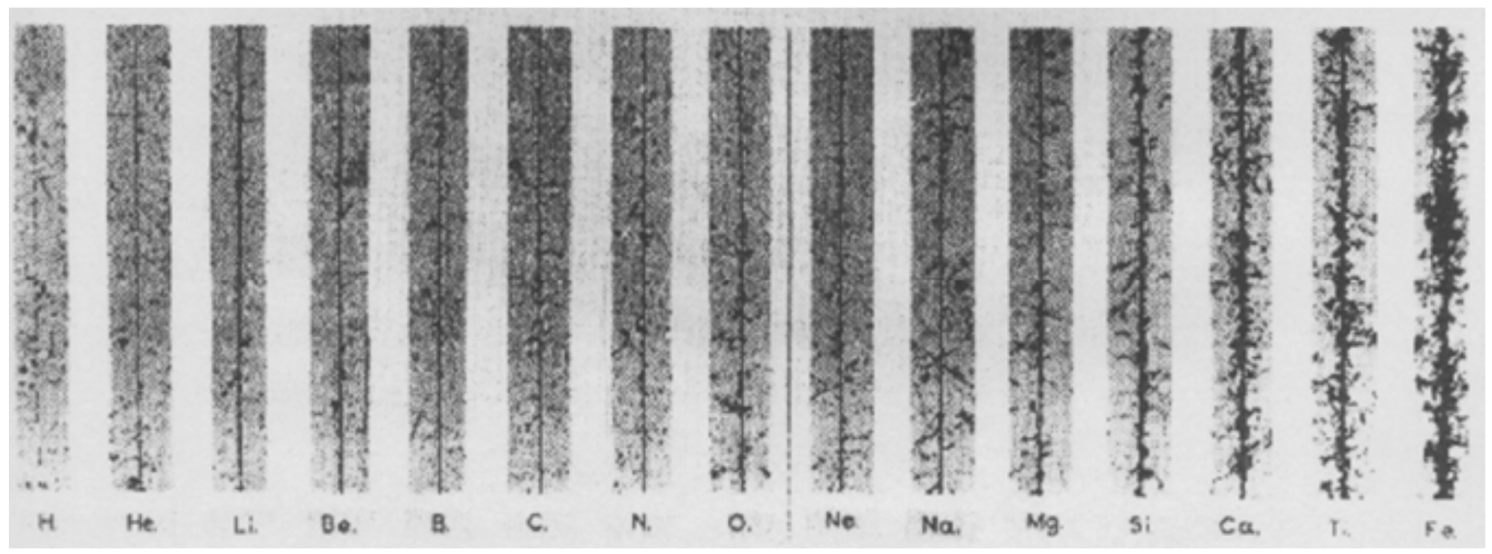
\includegraphics[width=0.75\linewidth]{Figures/EmulsionZ2.png}
    \caption{Nuclear emulsion tracks of cosmic-ray nuclei (H, He, Li, ... Fe), illustrating that the ionization density grows with $Z^2$. Adapted from the lecture slides (week 16, "Nuclear emulsion")}
    \label{fig:emulsionZ}
\end{figure}

The quantitative description of this ionization loss is given by the Bethe--Bloch
formula, which for a heavy charged particle (not an electron) reads, in the form
quoted in the lecture,
\begin{equation}
    \left\langle -\frac{dE}{dx} \right\rangle
    \;\approx\;
    K z^2 \frac{Z}{A} \frac{1}{\beta^2}
    \left[
        \frac{1}{2} \ln \frac{2 m_e c^2 \beta^2 \gamma^2 W_{\max}}{I^2} - \beta^2
    \right],
    \label{eq:bethe_bloch}
\end{equation}
where $z$ is the charge number of the incident particle, $Z$ and $A$ characterise
the absorber, $I$ is its mean excitation energy, $W_{\max}$ is the maximum energy
transferable to an atomic electron in a single collision, $K$ is a constant, and
$\beta = p/E$, $\gamma = E/M$ as usual. The energy loss falls steeply at low
velocity, passes through a broad minimum (the regime of minimum-ionizing
particles), and rises only logarithmically thereafter. Because a slow particle loses
energy ever more rapidly as it decelerates, the deposition is sharply peaked just
before the particle stops, a feature exploited in hadron tumor therapy. A
measurement of $dE/dx$ together with the momentum therefore separates particle
species, since at fixed momentum lighter particles are faster and ionize less than
heavier ones \cite[Ch.~2]{Amsler2018}.

\begin{figure}[htbp]
    \centering
    \begin{subfigure}[b]{0.45\textwidth}
        \centering
        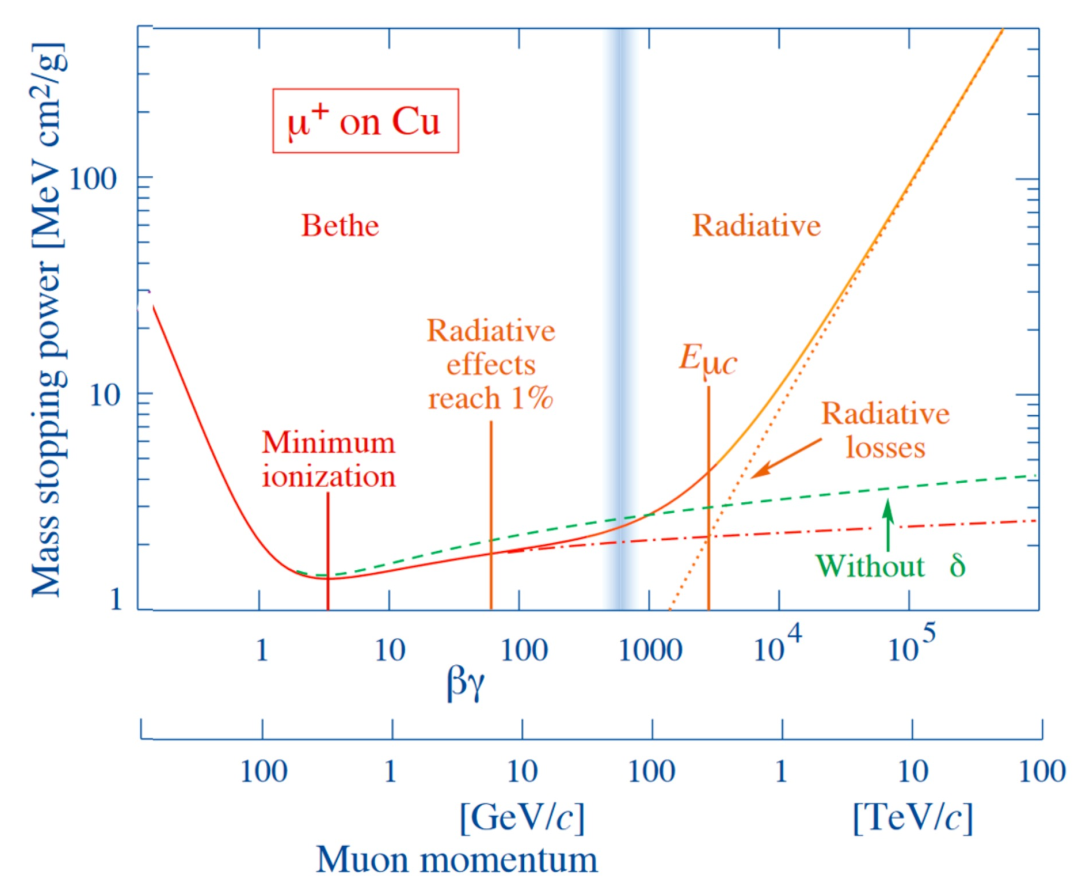
\includegraphics[width=\textwidth]{Figures/StoppingPower.png}
        \caption{Mass stopping power -dE/dx vs. beta-gamma for mu+ on Cu, showing the Bethe region, the minimum, and radiative losses at high energy}
        \label{fig:sub-first}
    \end{subfigure}
    \hfill
    \begin{subfigure}[b]{0.45\textwidth}
        \centering
        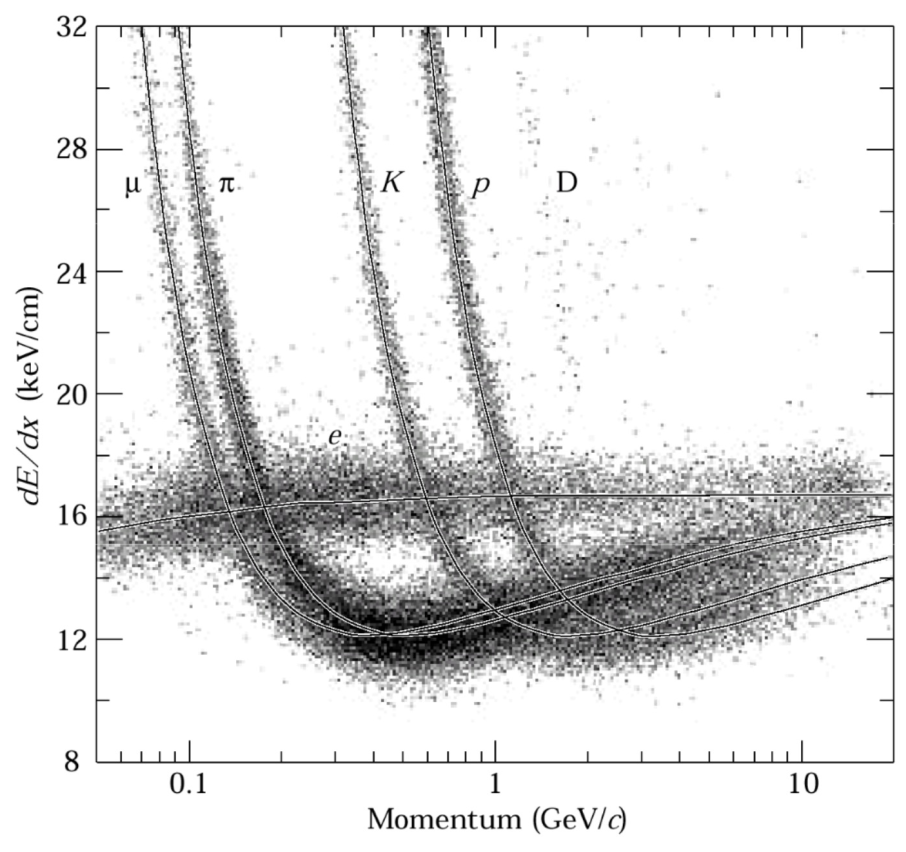
\includegraphics[width=\textwidth]{Figures/EnergyLoss.png}
        \caption{Measured dE/dx vs. momentum showing the separated mu, pi, K, p, D bands.}
        \label{fig:sub-second}
    \end{subfigure}
\end{figure}

The decisive cosmic-ray discovery for hadron physics was that of the charged pion.
A short-range mediator of the nuclear force had been postulated by Yukawa in 1935;
relating the range of the interaction, $R \sim 1\;\mathrm{fm}$, to the Compton
wavelength of the exchanged quantum yields a mass of order $200\,m_e$, that is
roughly $m_\pi \sim 200\;\mathrm{MeV}$ \cite[Ch.~2]{Amsler2018}. A particle found
in the cosmic radiation by Neddermeyer and Anderson in 1936 was at first taken to be
this quantum, but its failure to be absorbed by light nuclei showed it to be a
distinct, weakly interacting particle---the muon. The genuine Yukawa particle, the
charged pion with mass $m_\pi = 139.6\;\mathrm{MeV}$, was identified in 1947 by
Lattes, Occhialini and Powell using emulsions exposed at high altitude. The
characteristic decay sequence
\begin{equation}
    \pi^+ \;\to\; \mu^+ \;\to\; e^+
    \label{eq:pi_mu_e}
\end{equation}
was read directly from the emulsion: the constant range of the muon emerging from
the stopped pion signals the two-body decay $\pi^+ \to \mu^+ \nu_\mu$, the heavy
ionization near the ends of the pion and muon tracks marks their points of arrest,
and the faint track of the fast positron together with the Coulomb scattering of the
muon completes the identification \cite[Ch.~2]{Amsler2018}.

\subsection{The bubble chamber}

Emulsions provided exquisite spatial resolution but recorded events
indiscriminately and were laborious to scan. The bubble chamber, introduced in the
1950s, offered a controllable and repeatable alternative. Its active medium is a
liquid, often hydrogen, held just above its boiling point in a superheated state. A
charged particle crossing the liquid ionizes it along its path, and these ions act as
nucleation centers; a rapid decompression of the liquid then triggers boiling
precisely along the trajectory, so that a string of bubbles marks the track and can be
photographed. When the chamber sits in a magnetic field the trajectories curve, and
the sign and momentum of each particle follow from the sense and radius of
curvature. As in the emulsion, the bubble density along a track measures the
ionization and so contributes to particle identification through the combination of
curvature and ionization density. The principal limitation of the technique is its
speed: the compression cycle limits the repetition rate to about one expansion per
second or less \cite[Ch.~2]{Amsler2018}.

\begin{figure}[htbp]
    \centering
    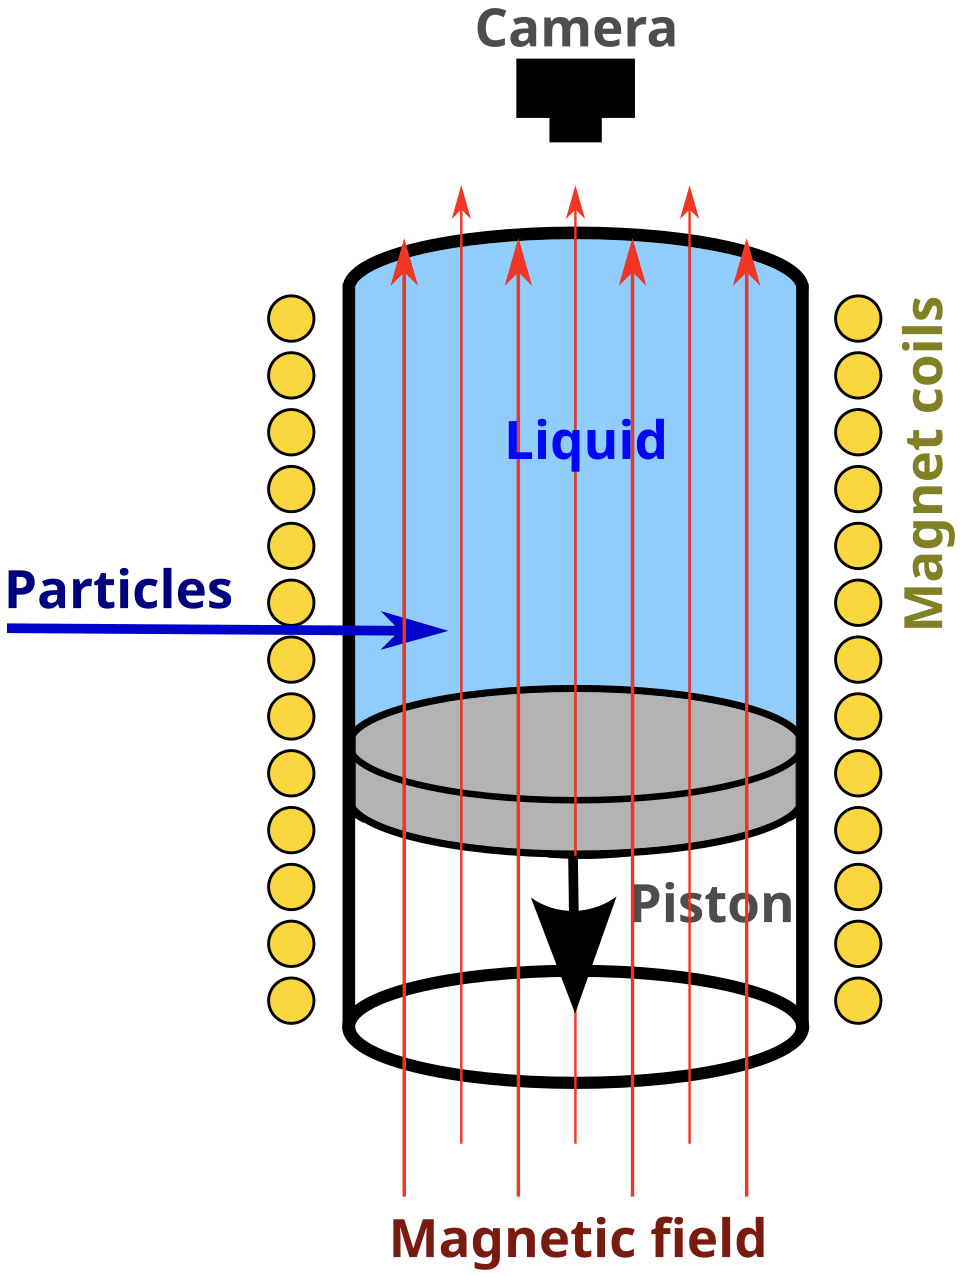
\includegraphics[width=0.5\linewidth]{Figures/BubbleChamber.png}
    \caption{Schematic of a bubble chamber: superheated liquid volume, incoming particle beam, piston for decompression, magnet coils producing the field, and an overhead camera.}
    \label{fig:bubblechamber}
\end{figure}

Such chambers were eventually built on a large scale. The Big European Bubble
Chamber (BEBC) at CERN, operated from the early 1970s, is a representative example;
analyses of its photographs continued into the 1990s. The hydrogen bubble chamber
became the workhorse instrument with which the strange baryons and the
$\Omega^-$ were established, as discussed in the next subsection.

\subsection{Hadron discovery at accelerators}

In the early 1950s particle accelerators became energetic enough to manufacture in
the laboratory the particles that had previously been glimpsed only in cosmic rays.
The Cosmotron at Brookhaven, for instance, accelerated protons to about
$3\;\mathrm{GeV}$, from which secondary pion beams of around $1.9\;\mathrm{GeV}$
could be derived. The defining experimental observation in these experiments was
the \emph{pairwise} production of the new ``strange'' particles: they were created
copiously, and always two at a time, in strong-interaction collisions, yet decayed
only slowly. This dichotomy was understood through a new additive quantum number,
strangeness $S$, conserved by the strong interaction that produces the particles but
violated by the weak interaction through which they decay---hence their description
as being produced in hadronic interactions but decaying weakly into hadrons
\cite[Ch.~2]{Amsler2018}.

The bubble-chamber and emulsion photographs of the period record a now-classic
catalogue of strange-particle production and decay. Neutral kaons were seen to
decay into pion pairs,
\begin{equation}
    K^0 \;\to\; \pi^+ \pi^- ,
\end{equation}
antiproton beams produced hyperon--antihyperon pairs such as
$\bar{p}p \to \bar{\Lambda}\Lambda$, and the charged and cascade hyperons revealed
themselves through their characteristic decay chains,
\begin{equation}
    \Sigma^+ \;\to\; p\,\pi^0 ,
    \qquad
    \Xi^- \;\to\; \Lambda \pi^- \;\to\; (p\,\pi^-)\,\pi^- .
\end{equation}
The cascade signature of the $\Xi^-$, decaying first to a $\Lambda$ and a pion and
then to a proton and a further pion, was particularly compelling evidence for a
hyperon carrying two units of strangeness. Later, neutrino beams---again analysed
in BEBC---extended this programme to weak production processes and to the charmed
hadrons \cite[Ch.~13]{Amsler2018}.

%% FIGURE SUGGESTION: Bubble-chamber or emulsion event displays of strange-particle
%% production, e.g. associated production of K and hyperons, with the decay chains
%% K0 -> pi+ pi-, ppbar -> Lambda Lambdabar, Sigma+ -> p pi0, and
%% Xi- -> Lambda pi- -> (p pi-) pi-. Adapted from the lecture slides (week 16,
%% "Discovery of hadrons") and Amsler (2018) Ch.~13.

\begin{figure}[htbp]
    \centering
    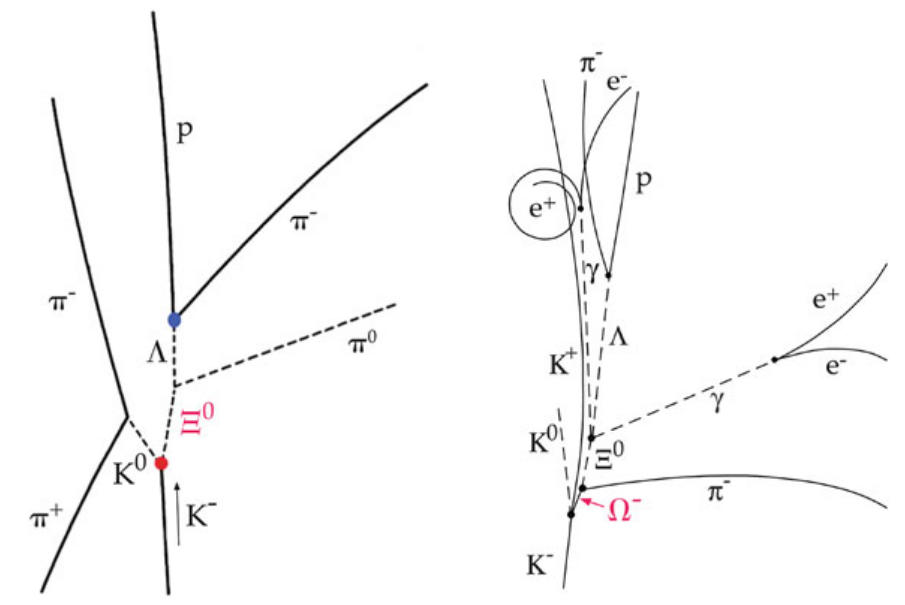
\includegraphics[width=0.75\linewidth]{Figures/BubbleChamberHyperonOmega.png}
    \caption{Bubble-chamber or emulsion event displays of strange-particle production, e.g. associated production of K and hyperons, with the decay chains $K_0 \rightarrow \pi^+ \pi^-$, $p \bar{p} \rightarrow \Lambda \bar{\Lambda}$, $\Sigma^+ -> p \pi_0$, and $\Xi^- -> \Lambda \pi^- \rightarrow (p \pi^-) \pi^-$}
    \label{fig:bublehyperon}
\end{figure}



\subsection{Determining particle properties}

Identifying a new hadron means measuring the set of characteristic quantum numbers
that distinguish it: its mass, its spin $J$, its parity $P$, its isospin $I$, its
baryon number $B$ and its strangeness $S$. Of these, the mass is the most directly
accessible. For a particle that decays into a set of measured daughters, or that is
produced in a reaction whose other products are measured, the mass follows from
energy--momentum conservation applied to the four-momenta. Writing the
four-momentum of particle $i$ as $P_i = (E_i, p_{x,i}, p_{y,i}, p_{z,i})$, the
invariant mass of a system reconstructed from two measured particles is
\begin{equation}
    m \;=\; \sqrt{\left(P_1 + P_2\right)^2},
    \label{eq:invariant_mass}
\end{equation}
where the square denotes the Lorentz-invariant scalar product of the total
four-momentum with itself. Because expression~\eqref{eq:invariant_mass} is a
Lorentz invariant, the same value is obtained in any reference frame, which is what
makes it the natural observable for identifying a resonance as a peak in a mass
spectrum \cite[Ch.~2]{Amsler2018}. The remaining quantum numbers $J$, $P$, $I$,
$B$ and $S$ are not read off a single track but are inferred from production and
decay patterns, angular distributions, and conservation laws; the determination of
the pion spin treated below is the prototypical example, and the strangeness
assignments follow from the associated-production rule of the previous subsection.

\subsection{Reconstructing masses: invariant mass and missing mass}

In practice two complementary strategies are used to evaluate
expression~\eqref{eq:invariant_mass}, depending on which particles a given detector
can measure. The first is a \emph{direct} reconstruction, in which all decay
products are detected and their four-momenta summed. A meson decaying to two
photons illustrates the method: in a calorimeter that records the energies and
directions of both photons, the squared invariant mass is simply
\begin{equation}
    m_{\gamma\gamma}^2 \;=\; \left(P_{\gamma,1} + P_{\gamma,2}\right)^2 ,
    \label{eq:direct_mass}
\end{equation}
and a histogram of $m_{\gamma\gamma}$ over many events shows peaks at the
$\pi^0$ and $\eta$ masses. The Crystal Barrel experiment at ELSA, for example,
isolates the $\eta \to \gamma\gamma$ signal in this way.

The second strategy is the \emph{missing-mass} method, used when the particle of
interest is not itself detected but recoils against a measured system. In the
photoproduction reaction $\gamma p \to \eta p$ with $\eta \to \gamma\gamma$, the
recoiling proton is measured in a tracking detector while the beam and target
four-momenta are known; the mass recoiling against the proton is then
\begin{equation}
    m_{\gamma\gamma}^2
    \;=\;
    \left(P_{\gamma,\mathrm{beam}} + P_{p,\mathrm{target}} - P_{p,\mathrm{meas}}\right)^2 .
    \label{eq:missing_mass}
\end{equation}
A peak in this missing mass at the $\eta$ mass confirms the reaction without any
direct observation of the meson's decay products. The CLAS experiment at Jefferson
Lab exemplifies this approach. The two methods are complementary: the direct method
demands full detection of the decay products, whereas the missing-mass method
trades that requirement for precise knowledge of the initial state and of the
recoiling system \cite[Ch.~2]{Amsler2018}.

%% FIGURE SUGGESTION: Side-by-side mass spectra illustrating the two methods.
%% (left) Direct gamma-gamma invariant mass spectrum (Crystal Barrel at ELSA) with
%% pi0 and eta peaks; (right) missing-mass spectrum (CLAS at Jefferson Lab) for
%% gamma p -> eta p showing pi0, eta, omega/rho and eta' peaks. Adapted from the
%% lecture slides (week 16, "Reconstructing meson masses -- an example").

\subsection{Determination of the pion spin}

The spin of the charged pion provides a clean illustration of how a quantum number
can be extracted from cross-section measurements alone, without any knowledge of
the underlying dynamics. The argument compares a reaction with its time reverse at
the same centre-of-mass energy,
\begin{equation}
    A: \quad pp \to \pi^+ d ,
    \qquad\qquad
    B: \quad \pi^+ d \to pp ,
    \label{eq:pi_spin_reactions}
\end{equation}
and rests on the principle of detailed balance. In a scattering process the
transition rate is given by Fermi's golden rule,
\begin{equation}
    W \;=\; \frac{2\pi}{\hbar}\,\lvert \mathcal{M}_{fi} \rvert^2 \rho_f ,
    \label{eq:golden_rule}
\end{equation}
where $\mathcal{M}_{fi}$ is the invariant transition amplitude connecting the
initial state $\lvert i \rangle$ to the final state $\lvert f \rangle$ and
$\rho_f$ is the density of final states. For the strong interaction
$\mathcal{M}_{fi}$ cannot be computed from first principles, and this is precisely
what the comparison of $A$ and $B$ is designed to circumvent
\cite[Ch.~2]{Amsler2018}.

Expressing the cross section of a two-body reaction
$a + b \to c + d$ through the squared amplitude and the appropriate spin
multiplicities and phase-space factors gives, in the notation of the lecture,
\begin{equation}
    \sigma(a + b \to c + d)
    \;=\;
    \lvert \mathcal{M}_{fi} \rvert^2
    \,\frac{(2 s_c + 1)(2 s_d + 1)}{v_i v_f}\, p_f^2 .
    \label{eq:sigma_general}
\end{equation}
Applying this to the two reactions in~\eqref{eq:pi_spin_reactions} with the proton
spin $s_p = \tfrac{1}{2}$ and the deuteron spin $s_d = 1$, and using the fact that
the strong interaction is invariant under both time reversal and space inversion---so
that the squared amplitudes are equal at the same centre-of-mass energy,
$\lvert \mathcal{M}_{fi} \rvert^2 = \lvert \mathcal{M}_{if} \rvert^2$---the unknown
amplitude cancels in the ratio. Care must be taken with the spin averaging:
reaction $A$ has initial spin multiplicity $(2 s_p + 1)^2 = 4$, of which only the
identical-particle factor $\tfrac{1}{2}$ survives in the final state, while reaction
$B$ carries the factor $(2 s_d + 1)(2 s_\pi + 1) = 3(2 s_\pi + 1)$. The result is
\begin{equation}
    \frac{\sigma(pp \to \pi^+ d)}{\sigma(\pi^+ d \to pp)}
    \;=\;
    \frac{3}{2}\,(2 s_\pi + 1)\,\frac{p_\pi^2}{p_p^2} ,
    \label{eq:pi_spin_ratio}
\end{equation}
where $p_\pi$ and $p_p$ are the centre-of-mass momenta of the pion and the proton
respectively \cite[Ch.~2]{Amsler2018}.

The right-hand side of~\eqref{eq:pi_spin_ratio} depends only on measurable momenta
and on the single unknown $s_\pi$. The first measurements, from Cartwright and
collaborators around 1950--1951 and from Durbin and collaborators in 1951---the
latter using a proton beam of kinetic energy $T_p = 340\;\mathrm{MeV}$ at the
Berkeley cyclotron---yielded a ratio consistent only with $s_\pi = 0$. The pion is
therefore a spinless particle, in keeping with its later interpretation as a
ground-state $q\bar{q}$ meson \cite[Ch.~2]{Amsler2018}.

%% FIGURE SUGGESTION: Comparison of the measured differential cross sections for
%% pi+ d -> pp and pp -> pi+ d (or the energy dependence of the two cross sections),
%% overlaid with the predictions for s_pi = 0 and s_pi = 1, demonstrating the clear
%% preference for s_pi = 0. Adapted from the lecture slides (week 16,
%% "Determination of the pion-spin") and the data of Cartwright et al. and
%% Durbin et al.

\subsection{Ordering the particle zoo: towards the quark model}

By the late 1950s the experimental programmes described above had produced an
embarrassment of riches. So many strongly interacting particles had been found that
they could no longer all be regarded as elementary, a situation captured in Fermi's
quip that had he been able to remember the names of all the particles he would have
become a botanist, and in Lamb's wry suggestion that the discovery of a new particle
ought to be punished rather than rewarded. The proliferation---the so-called
``particle zoo''---demanded an organising principle analogous to the periodic table
of the chemical elements, and the very existence of such a regularity would point,
as it had for atoms, to an underlying substructure \cite[Ch.~1]{Amsler2018}.

The resolution came from the use of symmetry and group theory. Gell-Mann and, in a
related development, Ne'eman recognised around 1961--1964 that the known hadrons
fall naturally into multiplets of the approximate flavour symmetry group
$\mathrm{SU}(3)_f$, a scheme that Gell-Mann named the Eightfold Way
\cite[Ch.~2]{HalzenMartin1984}. The fundamental representation of $\mathrm{SU}(3)$
is three-dimensional, and Gell-Mann and, independently, Zweig proposed in 1964 that
these three basis states correspond to physical (at the time hypothetical)
constituents, the quarks $u$, $d$ and $s$. Gell-Mann drew the name from a line in
James Joyce's \textit{Finnegans Wake}, ``Three quarks for Muster Mark''. In this
picture the mesons, which carry integer spin, are quark--antiquark combinations
$q\bar{q}$, while the baryons, which carry half-integer spin, are three-quark
combinations $qqq$ \cite[Ch.~1]{Amsler2018}.

%% FIGURE SUGGESTION: The lightest SU(3)_f weight diagrams: the pseudoscalar meson
%% nonet (qqbar) and the spin-1/2 baryon octet (qqq), plotted in the strangeness vs.
%% charge plane, with the original excerpt from Gell-Mann's 1964 "A Schematic Model
%% of Baryons and Mesons". Adapted from the lecture slides (week 16, "Order in the
%% zoo") and Amsler (2018) Ch.~7, Ch.~13.

The classifying power of the scheme was striking: the lightest pseudoscalar and
vector mesons group into octets and singlets, and the lightest baryons into an octet
and a decuplet. Its most celebrated success was predictive rather than merely
descriptive. The pattern of the spin-$\tfrac{3}{2}$ baryon decuplet left a single
vacant position, a triply strange state, whose mass could be read off from the
equal spacing of the other members. The corresponding particle, the $\Omega^-$, was
duly observed in a bubble chamber at Brookhaven in 1964 with a mass close to the
predicted value, a confirmation that transformed the quark model from a bookkeeping
device into a description of genuine substructure \cite[Ch.~7]{Amsler2018}. The
group-theoretical machinery that underlies these multiplets---isospin, the
construction of $\mathrm{SU}(N)$ representations, and the weight diagrams---is the
subject of the following chapter.
\section{Groups and Isospin}

\subsection{Addition of spin}

\subsection{SU(N) multiplets and Young tableaux}
\section{Mesons, wavefunctions and nomenclature}
\label{sec:mesons}

The previous chapter organized the light hadrons into the irreducible
representations of $\mathrm{SU(3)}_{F}$ and used the Gell-Mann--Okubo formula to
account for the mass splittings within the baryon multiplets. This chapter
specializes that machinery to the $q\bar q$ mesons. We first complete the catalogue
of meson quantum numbers begun in Sect.~\ref{sec:groups} by deriving the $G$ parity
and listing the accessible and the ``exotic'' $J^{PC}$ combinations. We then build
the meson nonet and analyze the symmetry of its wavefunctions in the combined
spin--flavor group $\mathrm{SU}(6)$, discuss the mixing of the two neutral
isoscalars and the special case of ideal mixing, fix the mixing angle from the meson
masses, and examine the dynamical consequences of the quark-line structure through
the Okubo--Zweig--Iizuka rule and the leptonic widths of the vector mesons. The
chapter closes with the modern naming scheme and with the $\eta$ meson as a precision
laboratory for the strong interaction and for physics beyond the Standard Model.

% ============================================================
\subsection{Quantum numbers and wavefunctions}
\label{subsec:qnumbers}

A meson is a bound quark--antiquark pair, the strong-interaction analogue of
positronium. Its internal wavefunction factorizes into a radial, an angular and a
spin part,
\begin{equation}
    \psi(\vec r,\vec s) = R(r)\,Y_{lm}(\theta,\phi)\,\chi(\vec s),
    \label{eq:meson_wavefunction}
\end{equation}
so that the total quark spin $S = s_q + s_{\bar q}$ takes the values $0$ or $1$ and
combines with the relative orbital angular momentum $L$ to give the meson spin
$J = L \oplus S$, with $|L-S| \le J \le L+S$. The state is conventionally labeled in
the spectroscopic notation $n^{\,2S+1}L_J$, where $n$ is the radial quantum number
and $L = S, P, D, \dots$ stands for $L = 0, 1, 2, \dots$
\cite[Ch.~2]{Amsler2018}. The parity and charge-conjugation eigenvalues of a
$q\bar q$ pair, derived in Sect.~\ref{sec:groups}, are
\begin{equation}
    P = (-1)^{L+1},
    \qquad
    C = (-1)^{L+s},
    \label{eq:meson_PC}
\end{equation}
the $C$ parity being defined only for the electrically neutral members with hidden
flavor ($S = C = B = 0$), for which the particle is its own antiparticle
\cite[Ch.~3]{Amsler2018}.

Charged mesons, and more generally any state with $I_{3} \neq 0$, cannot be eigenstates
of $C$ alone, since charge conjugation flips the sign of $I_{3}$ and therefore maps,
for instance, a $\pi^+$ onto a $\pi^-$,
\begin{equation}
    C\,\ket{\pi^+} = \eta_C\,\ket{\pi^-}.
\end{equation}
The eigenvalue can nevertheless be recovered by following the charge conjugation
with a rotation by $180^\circ$ about the $2$-axis in isospin space, represented by
the operator $R_U = \exp(i\pi I_2)$, which restores $I_{3}$ and hence the original
charge. The combined operation defines the \emph{$G$ parity}
\begin{equation}
    G = C\,e^{i\pi I_2},
    \label{eq:Gparity_def}
\end{equation}
of which the whole isospin multiplet is now a common eigenstate. For an isospin-$I$
multiplet the rotation contributes a factor $(-1)^I$, so that for a $q\bar q$ system
\begin{equation}
    G = C\,(-1)^I = (-1)^{L+s+I},
    \label{eq:Gparity}
\end{equation}
combining Eqs.~\eqref{eq:meson_PC} and \eqref{eq:Gparity_def}
\cite[Ch.~3]{Amsler2018}. Because both $C$ and isospin are conserved by the strong
interaction, $G$ parity is conserved as well; it is a practical bookkeeping device
rather than an independent symmetry. A particularly useful consequence is that a
system of $n$ pions has $G(n\pi) = (-1)^n$, which dictates that the $\rho$ ($G=+1$)
decays into two pions and the $\omega$ ($G=-1$) into three. The $G$ parity is not
defined for the $K$, $D$ and $B$ mesons, which carry open flavor
\cite[Ch.~3]{Amsler2018}.

% ------------------------------------------------------------
\subsubsection{Identical bosons in the final state}
\label{subsubsec:bose-symmetry}

The $G$-parity rule $G(n\pi) = (-1)^n$ is a necessary condition, not a sufficient one.
Whenever two or more of the final-state mesons are \emph{identical}, Bose symmetry
imposes a further restriction which forbids decays that $G$ parity alone would allow.
It is the exact counterpart of the Pauli argument used for the baryons in
Sect.~\ref{sec:baryons-color}: the total wavefunction of a system of identical bosons
must be \emph{symmetric} under their exchange.

For two identical pseudoscalars the wavefunction consists of a spatial part carrying
$(-1)^{L}$ and an isospin part. Exchange symmetry therefore requires the isospin
function to have the same symmetry as the spatial one. Coupling two $I=1$ pions gives
\begin{equation}
    \mathbf{3}\otimes\mathbf{3} = \mathbf{5}_S \oplus \mathbf{3}_A \oplus \mathbf{1}_S ,
    \label{eq:pipi_isospin}
\end{equation}
so $I = 2$ and $I = 0$ are symmetric while $I = 1$ is antisymmetric. A $\pi\pi$ state
therefore satisfies
\begin{equation}
    (-1)^{L} = (-1)^{I} \quad\Longrightarrow\quad L + I \;\text{even}.
    \label{eq:pipi_symmetry}
\end{equation}

Two consequences are used repeatedly. First, since a two-pion state has
$P = (-1)^{L}$ and, when neutral, $C = (-1)^{L}$, the combination $J^{PC} = 1^{--}$
requires $L = 1$ and hence, by Eq.~\eqref{eq:pipi_symmetry}, $I = 1$. The $\rho$ meson
duly decays to $\pi\pi$. Second---and this is the part $G$ parity does not capture---the
particular final state $\pi^0\pi^0$ consists of two \emph{identical} particles, for which
only the symmetric isospin combinations survive. The relevant Clebsch--Gordan coefficient
vanishes,
\begin{equation}
    \braket{1,0;1,0}{1,0} = 0 ,
    \label{eq:pi0pi0_CG}
\end{equation}
so a state of odd $L$ cannot decay into two neutral pions at all. Amsler reaches the
same conclusion from charge conjugation: for a pair of identical bosons $C$ permutes the
two particles, and Bose--Einstein symmetry then forces $L + s$ to be even, so that a
self-conjugate pair such as $\pi^0\pi^0$ or $\gamma\gamma$ is an eigenstate of $C$ with
eigenvalue $+1$ \cite[Ch.~3]{Amsler2018}. The same argument excludes spin $1$ for the
$\pi^0\pi^0$ system observed in $K_S$ decay \cite[Ch.~2]{Amsler2018}. Hence
\begin{equation*}
    \rho^0 \nrightarrow \pi^0\pi^0,
    \qquad
    \omega \nrightarrow \pi^0\pi^0 ,
\end{equation*}
even though $\rho^0 \to \pi^+\pi^-$ proceeds freely. Equivalently: two identical
pseudoscalars in a relative $L=1$ state would have to be antisymmetric in space and
symmetric in every other label, which Bose statistics forbids.

The same reasoning extends to three identical pions. The decay $\phi \to \pi^0\pi^0\pi^0$
is not forbidden by $G$ parity---$G(3\pi) = -1$ matches $G(\phi) = -1$---but it is
forbidden by the combination of $C$ parity and Bose symmetry. A system of three identical
neutral pions must be totally symmetric, and a totally symmetric $3\pi^0$ state cannot
carry the $J^{PC} = 1^{--}$ of the $\phi$. The observed decay is
$\phi \to \pi^+\pi^-\pi^0$, where the pions are not all identical and the constraint
relaxes. Arguments of exactly this kind are what fix the allowed initial states in
proton--antiproton annihilation (Sect.~\ref{subsec:annihilation}).

Equations~\eqref{eq:meson_PC} and \eqref{eq:Gparity} restrict the quantum numbers
that a simple $q\bar q$ pair can carry. Running through the lowest values of $L$ and
$S$ gives the accessible combinations
\begin{equation}
    J^{PC}(q\bar q) = 0^{-+},\,0^{++},\,1^{--},\,1^{+-},\,1^{++},\,
                      2^{--},\,2^{-+},\,2^{++},\,3^{--},\,3^{+-},\,3^{++},\,\dots
    \label{eq:allowed_JPC}
\end{equation}
while the values
\begin{equation}
    J^{PC} = 0^{--},\,0^{+-},\,1^{-+},\,2^{+-},\,3^{-+},\,\dots
    \label{eq:exotic_JPC}
\end{equation}
cannot be reached by any $L,S$ assignment. A state observed with one of these
\emph{exotic} quantum numbers cannot be a conventional meson and must instead be a
glueball ($gg$), a hybrid ($q\bar q g$), a meson--meson molecule, or a multiquark
state such as a tetraquark ($q\bar q q\bar q$); these configurations are taken up in
a later chapter \cite[Ch.~4]{Amsler2018}. The catalogue \eqref{eq:exotic_JPC}
thereby turns the elementary counting of $q\bar q$ quantum numbers into an
experimental search strategy for physics beyond the naive quark model.

\begin{figure}[htbp]
    \centering
    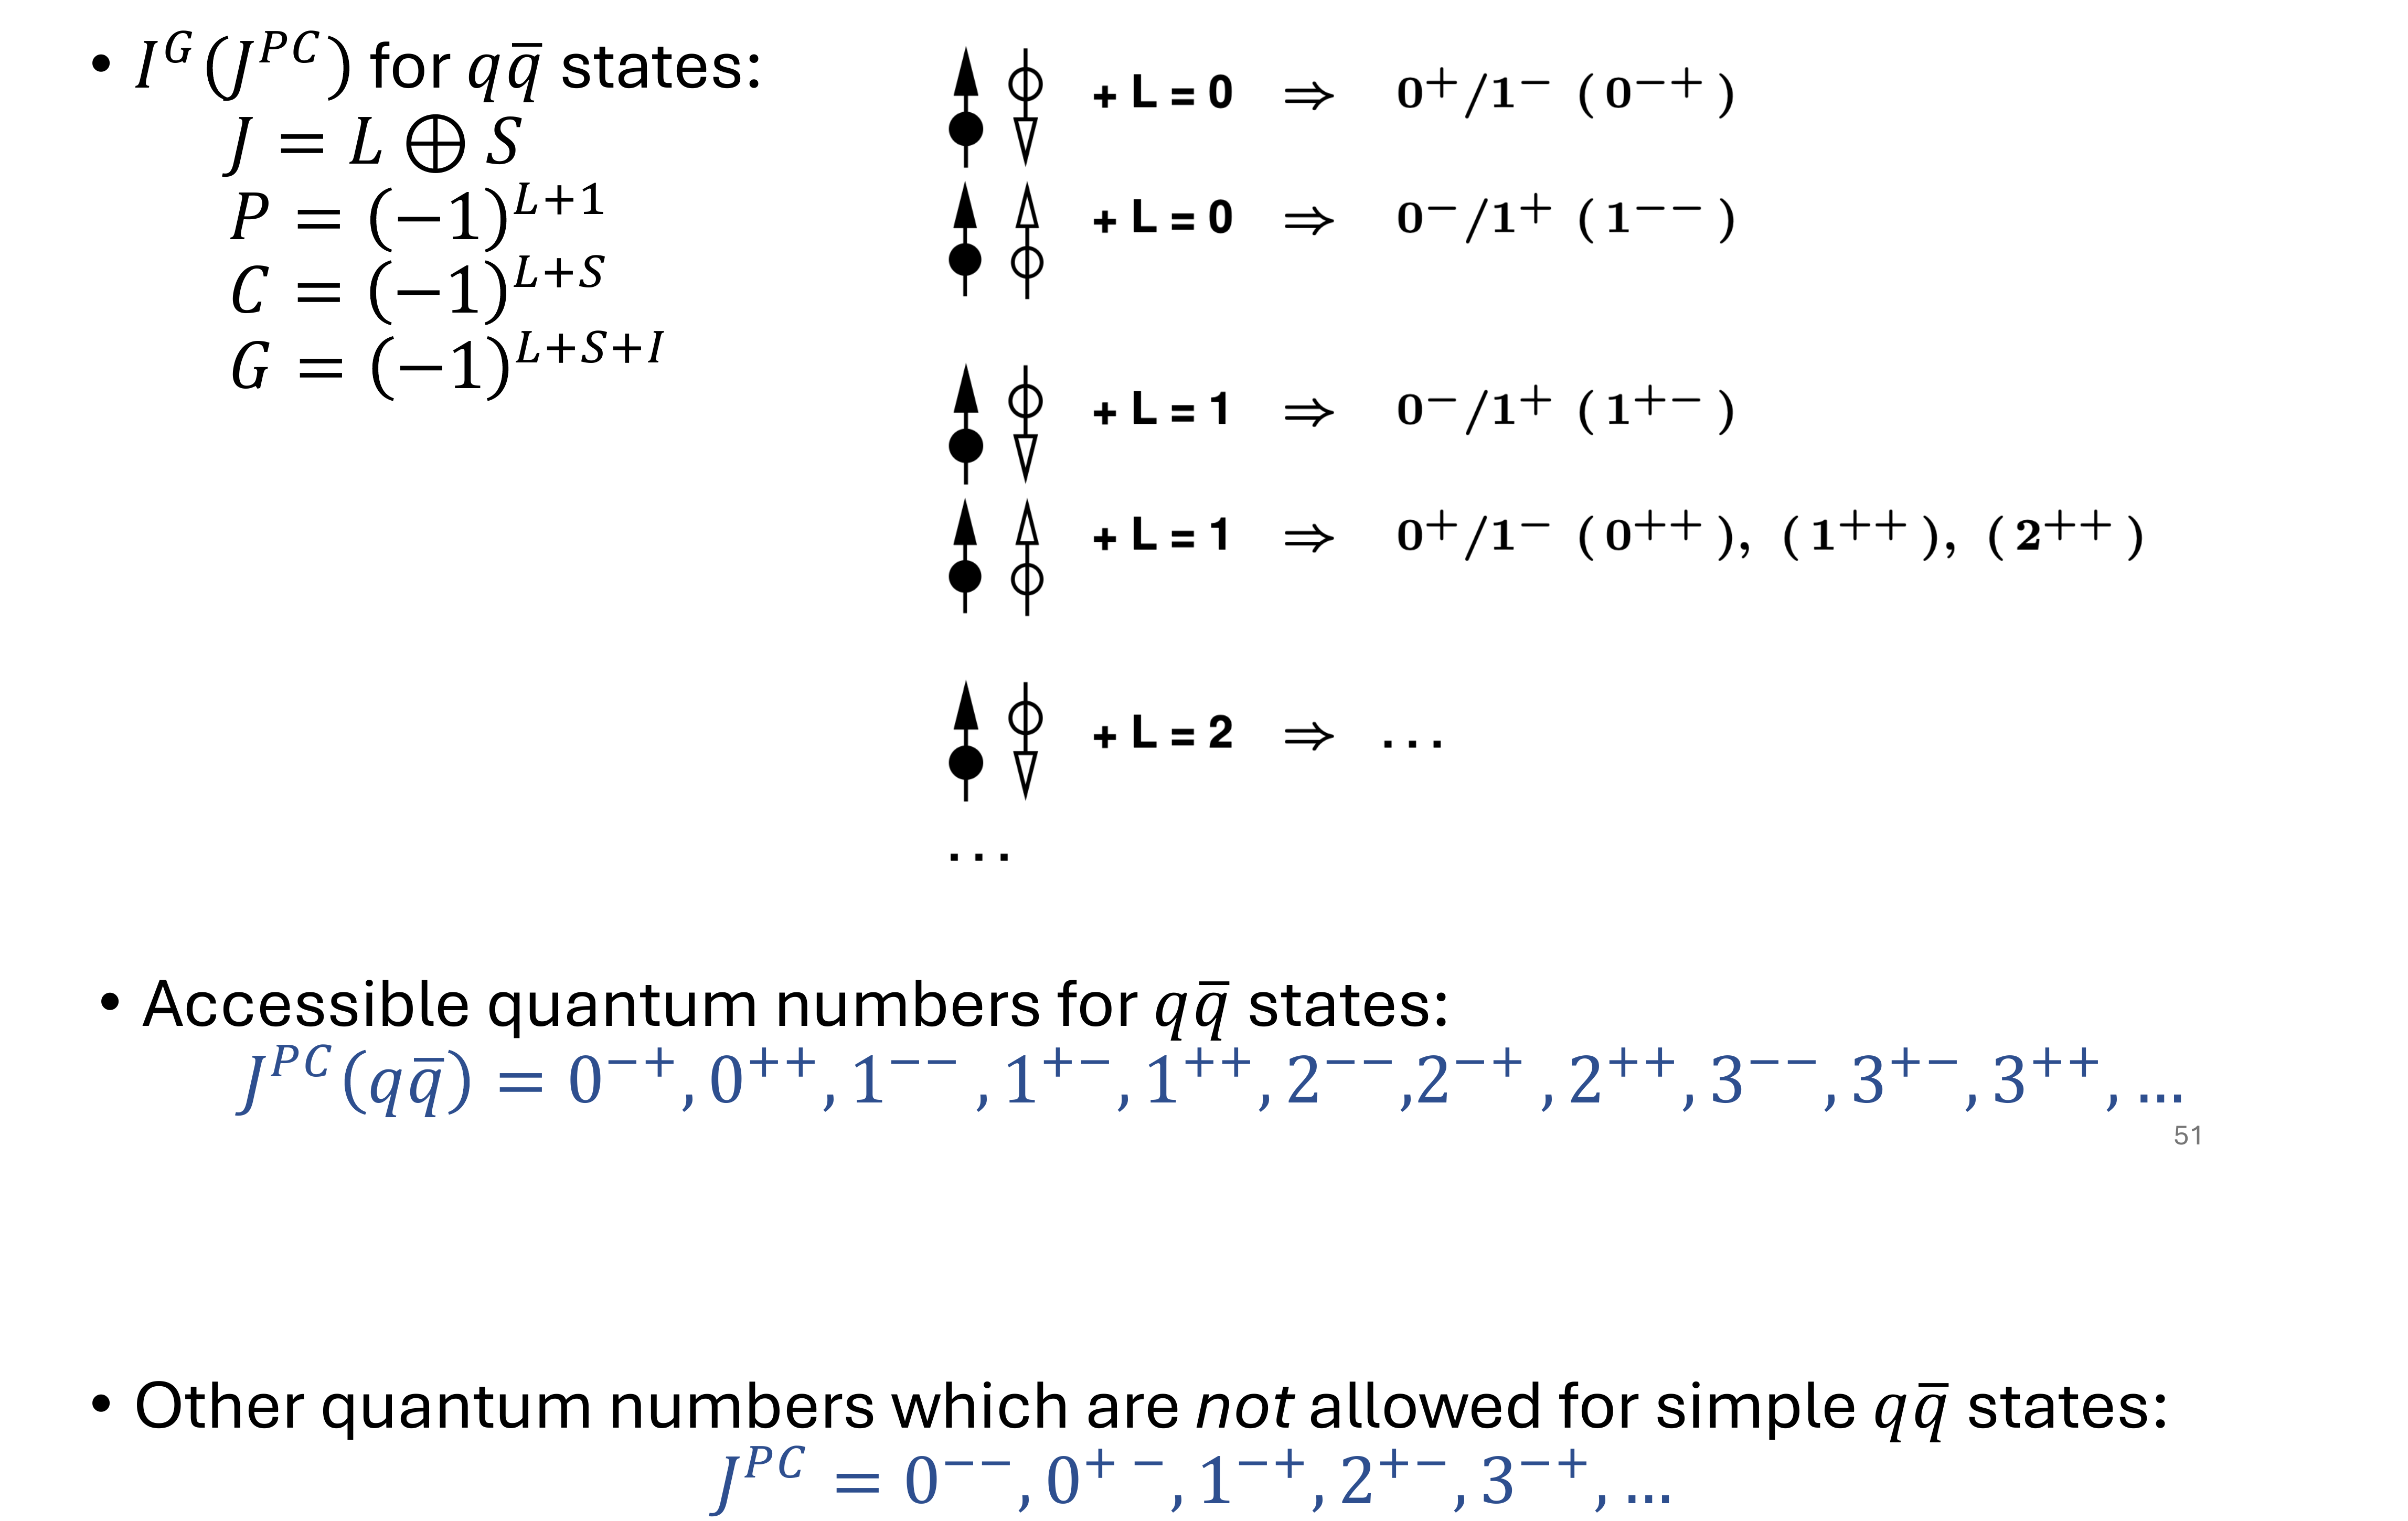
\includegraphics[width=0.85\linewidth]{Figures/qqbar_JPC_ladder.png}
    \caption{Spin and orbital angular momentum of a $q\bar q$ pair and the
    resulting $J^{PC}$ quantum numbers. The combinations
    in the lower block (Eq.~\eqref{eq:exotic_JPC}) cannot be formed by a simple
    quark--antiquark pair and are termed exotic. Adapted from the lecture
    slides (week 19, "Possible quantum numbers of $q\bar q$ states").}
    \label{fig:jpc_ladder}
\end{figure}

% ============================================================
\subsection{Mesons}
\label{subsec:mesons}

With three flavors of light quark the fundamental representation of
$\mathrm{SU(3)}_{F}$ is the triplet $(u,d,s)$, and a $q\bar q$ pair lives in the product
\begin{equation}
    \mathbf{3}\otimes\overline{\mathbf{3}} = \mathbf{1}\oplus\mathbf{8},
    \label{eq:nonet_decomp}
\end{equation}
so that, for a given $J^{PC}$, the nine quark--antiquark combinations group into an
octet and a singlet---the meson \emph{nonet} \cite[Ch.~7]{Amsler2018}. The six
states on the periphery of the weight diagram carry open flavor and are uniquely
fixed; for the pseudoscalars they are the kaons $K^+ = u\bar s$, $K^0 = d\bar s$,
$\bar K^0 = s\bar d$, $K^- = s\bar u$ together with the charged pions
$\pi^+ = u\bar d$ and $\pi^- = d\bar u$. The three states sitting at the center of
the hexagon all have $I_{3} = Y = 0$ and must be disentangled. The neutral member of
the isotriplet cannot contain an $s\bar s$ component and is
\begin{equation}
    \ket{8,3} = \tfrac{1}{\sqrt 2}\,\ket{u\bar u - d\bar d}
    \;\;(\,\widehat{=}\;\pi^0\;\text{or}\;\rho^0\,),
    \label{eq:pi0_state}
\end{equation}
while the two isoscalars are the $\mathrm{SU}(3)$ singlet and the isoscalar member of
the octet, obtained by Gram--Schmidt orthogonalisation,
\begin{align}
    \ket{1,1} &= \tfrac{1}{\sqrt 3}\,\ket{u\bar u + d\bar d + s\bar s}, \\
    \ket{8,1} &= \tfrac{1}{\sqrt 6}\,\ket{u\bar u + d\bar d - 2s\bar s},
    \label{eq:singlet_octet}
\end{align}
the singlet being the flavor-symmetric, $\mathrm{SU}(3)$-invariant combination and
the octet state the one orthogonal both to it and to Eq.~\eqref{eq:pi0_state}
\cite[Ch.~7]{Amsler2018}.

The permutation symmetry of the meson wavefunction is most transparent in the
combined spin--flavor group obtained by merging the flavor group
$\mathrm{SU(3)}_{F}$ with the spin group $\mathrm{SU}(2)_{\text{spin}}$ into
$\mathrm{SU}(6)$, whose fundamental representation contains the six states
$u\!\uparrow, d\!\uparrow, s\!\uparrow, u\!\downarrow, d\!\downarrow, s\!\downarrow$.
A meson wavefunction factorizes as
\begin{equation}
    \psi = \Phi_{\text{flavor}}\,\chi_{\text{spin}}\,\lambda_{\text{color}}\,R(\vec{r}\,),
    \label{eq:su6_wavefunction}
\end{equation}
where the color part $\lambda_{\text{color}}$ is the $q\bar q$ singlet. It is
totally symmetric and carries no free index, so it plays no role in the symmetry
counting below and is suppressed from here on.
and since the flavor part decomposes according to Eq.~\eqref{eq:nonet_decomp} into
symmetric and antisymmetric combinations $\Phi_S, \Phi_A$, while the two spins
combine into symmetric ($\chi_S$, $s=1$) and antisymmetric ($\chi_A$, $s=0$) parts,
there are four possible products: the symmetric $\Phi_S\chi_S$ and $\Phi_A\chi_A$,
and the antisymmetric $\Phi_S\chi_A$ and $\Phi_A\chi_S$
\cite[Ch.~7]{Amsler2018}. The physically realized symmetry is fixed by charge
conjugation, which exchanges quark and antiquark and acts on the flavor part with
the factor $(-1)^{L+s}$ of Eq.~\eqref{eq:meson_PC}. For the pseudoscalar ground
states ($L = s = 0$, spin function $\chi_A$),
\begin{equation}
    C\ket{\pi^0} = C(\Phi\chi) = (-1)^{0+0}\,\Phi\chi = +\Phi\chi = \Phi_S\chi
    \;\;\Longrightarrow\;\; \psi(\pi^0) = \Phi_S\chi_A,
\end{equation}
which is overall antisymmetric, while for the vector ground states ($L=0$, $s=1$,
spin function $\chi_S$),
\begin{equation}
    C\ket{\rho^0} = (-1)^{0+1}\,\Phi\chi = -\Phi\chi = \Phi_A\chi
    \;\;\Longrightarrow\;\; \psi(\rho^0) = \Phi_A\chi_S,
\end{equation}
again antisymmetric overall. Consistently, the neutral isovector
Eq.~\eqref{eq:pi0_state} is realized as the flavor-symmetric combination for the
pseudoscalar and as the flavor-antisymmetric combination for the vector
\cite[Ch.~7]{Amsler2018}.

\begin{figure}[htbp]
    \centering
    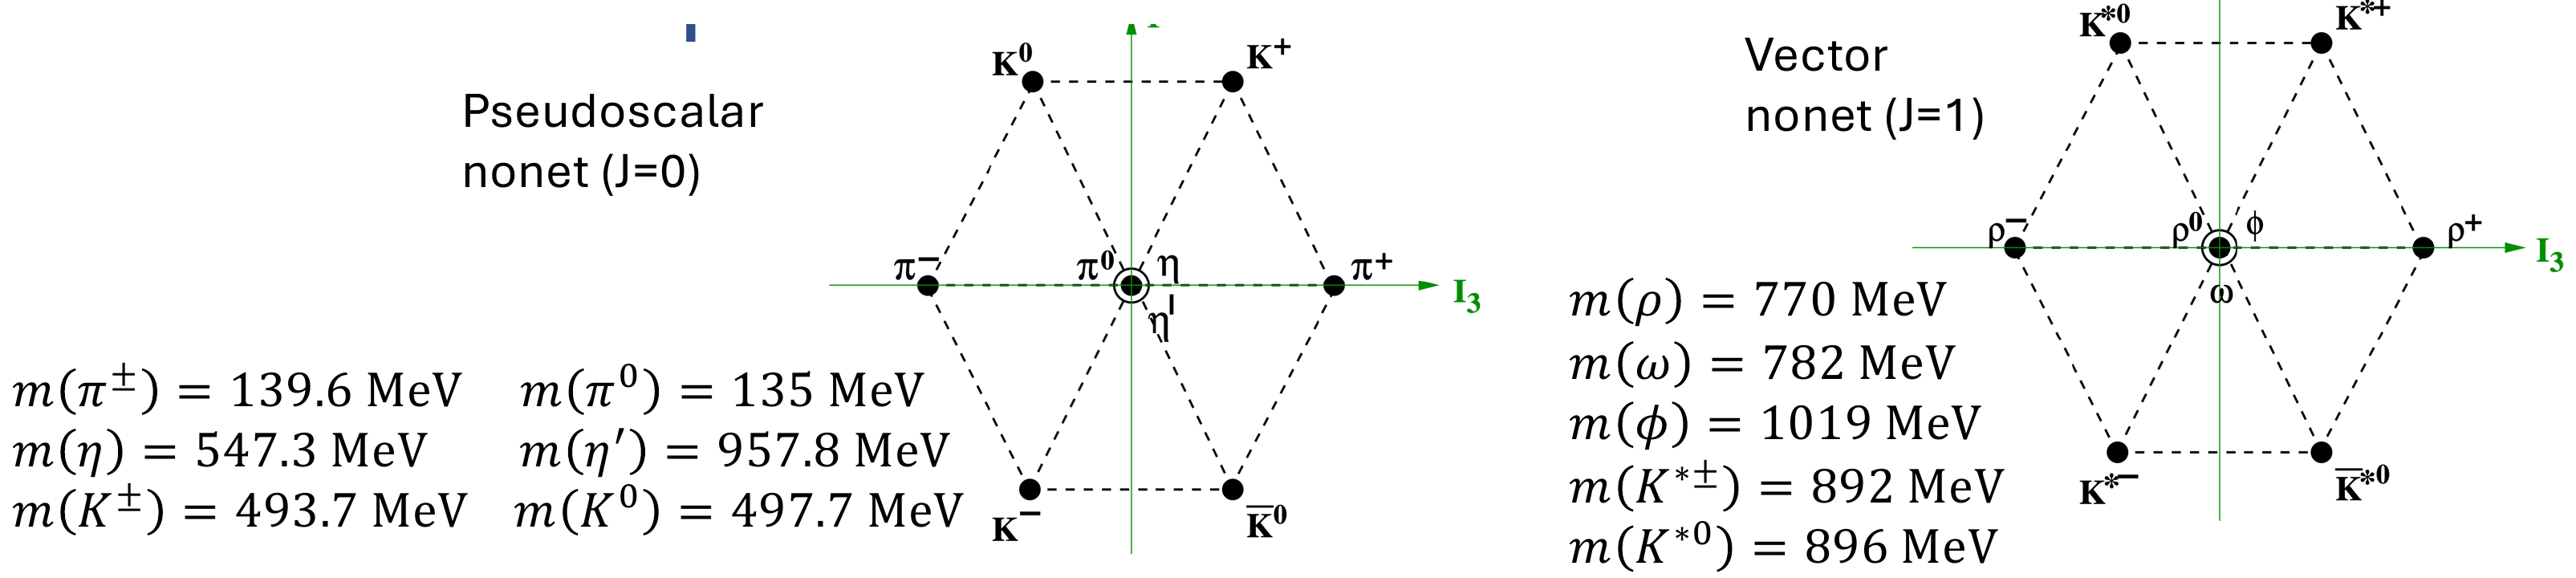
\includegraphics[width=0.9\linewidth]{Figures/meson_nonets.png}
    \caption{Weight diagrams of the pseudoscalar ($J^{PC} = 0^{-+}$) and vector
    ($J^{PC} = 1^{--}$) meson nonets in the $(I_3, Y)$ plane. The six
    open-flavor states lie on the periphery of the hexagon; the three neutral,
    flavorless states occupy the center. Adapted from the lecture slides
    (week 19, "Meson multiplets").}
    \label{fig:meson_nonets}
\end{figure}

% ============================================================
\subsection{Nonets and ideal mixing}
\label{subsec:nonets}

The two central isoscalars $\ket{8,1}$ and $\ket{1,1}$ share all conserved quantum
numbers ($Q = I = S = 0$) and therefore mix. The physically observed states are the
orthogonal superpositions
\begin{align}
    \ket{f_A} &= \cos\theta\,\ket{8,1} - \sin\theta\,\ket{1,1}, \notag\\
    \ket{f_B} &= \sin\theta\,\ket{8,1} + \cos\theta\,\ket{1,1},
    \label{eq:nonet_mixing}
\end{align}
with a single mixing angle $\theta$ that must be determined from experiment by
comparing masses, decays and production properties \cite[Ch.~5]{Amsler2018}. A
distinguished value is \emph{ideal mixing},
\begin{equation}
    \tan\theta = \frac{1}{\sqrt 2}
    \;\;\Longleftrightarrow\;\;
    \theta = 35.3^\circ,
    \label{eq:ideal_mixing}
\end{equation}
for which the $s\bar s$ component decouples completely from the light quarks, so that
one physical isoscalar becomes pure strange and the other a pure $u,d$ combination,
\begin{equation}
    \ket{f_A} = -\ket{s\bar s},
    \qquad
    \ket{f_B} = \tfrac{1}{\sqrt 2}\,\ket{u\bar u + d\bar d}.
    \label{eq:ideal_states}
\end{equation}

The vector nonet is very close to ideal mixing. The near degeneracy
$m(\rho(770)) \approx m(\omega(782))$ already signals that the $\omega$ shares the
light-quark content of the $\rho^0$, and the assignment
$\ket{\omega} = \tfrac{1}{\sqrt 2}\ket{u\bar u + d\bar d}$,
$\ket{\phi} = -\ket{s\bar s}$ follows with $\theta_V \approx 35.3^\circ$
\cite[Ch.~5]{Amsler2018}. The pseudoscalar nonet is the conspicuous exception: its
mixing angle lies in the range $-10^\circ$ to $-20^\circ$, far from ideal, so that
the $\eta$ and $\eta'$ are close to the pure octet and singlet states of
Eq.~\eqref{eq:singlet_octet}. The reason is dynamical. The mixing is driven by the
annihilation of the $q\bar q$ pair into intermediate gluons; for the $0^{-+}$
isoscalars a two-gluon intermediate state is allowed, generating a large
perturbation, whereas for the $1^{--}$ isoscalars the Landau--Yang theorem forbids a
spin-$1$ state from coupling to two massless spin-$1$ gluons, so at least three gluons are
required and the perturbation is strongly suppressed \cite[Ch.~5]{Amsler2018}.%
\footnote{Amsler calls this the ``Fermi--Yang theorem'' at this point in Sect.~5.2,
but cites Landau (1948) and Yang (1950) as the reference and uses the standard name
Landau--Yang everywhere else, including the proof in his Appendix~A. The Fermi--Yang
model is the unrelated 1949 proposal of the pion as an $N\bar N$ bound state.} This
is why the vectors mix ideally while the pseudoscalars do not. The measured masses
of the two ground-state nonets,
\begin{equation}
\begin{aligned}
    &m(\pi^\pm) = 139.6,\;\; m(\pi^0) = 135,\;\;
     m(\eta) = 547.3,\;\; m(\eta') = 957.8,\\
    &m(K^\pm) = 493.7,\;\; m(K^0) = 497.7
    \qquad\text{(pseudoscalars)},\\[2pt]
    &m(\rho) = 770,\;\; m(\omega) = 782,\;\; m(\phi) = 1019,\;\;
     m(K^{*\pm}) = 892,\;\; m(K^{*0}) = 896
     \quad\text{(vectors)},
\end{aligned}
\label{eq:nonet_masses}
\end{equation}
(in MeV) are the inputs to the mass formulae of the next subsection
\cite[Ch.~5]{Amsler2018}.

\begin{figure}[htbp]
    \centering
    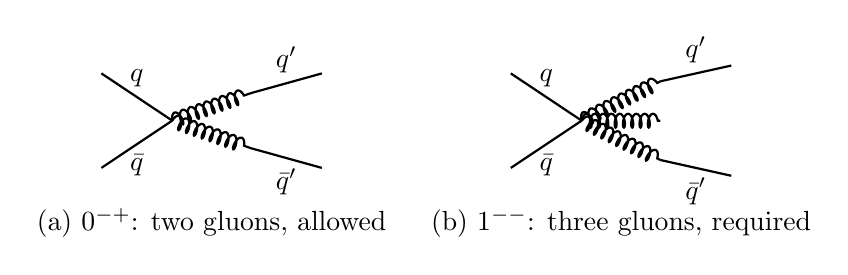
\begin{tikzpicture}[thick, scale=1.0]
        % Left: 2-gluon process (pseudoscalar, allowed)
        \begin{scope}
            \draw (-1.4,0.6) -- (-0.5,0) node[midway, above] {$q$};
            \draw (-1.4,-0.6) -- (-0.5,0) node[midway, below] {$\bar q$};
            \draw[decorate,decoration={coil,aspect=0.4,segment length=3pt}]
                (-0.5,0) -- (0.5,0.35);
            \draw[decorate,decoration={coil,aspect=0.4,segment length=3pt}]
                (-0.5,0) -- (0.5,-0.35);
            \draw (0.5,0.35) -- (1.4,0.6) node[midway, above] {$q'$};
            \draw (0.5,-0.35) -- (1.4,-0.6) node[midway, below] {$\bar q'$};
            \node at (0,-1.3) {(a) $0^{-+}$: two gluons, allowed};
        \end{scope}
        % Right: 3-gluon process (vector, required)
        \begin{scope}[xshift=5.2cm]
            \draw (-1.4,0.6) -- (-0.5,0) node[midway, above] {$q$};
            \draw (-1.4,-0.6) -- (-0.5,0) node[midway, below] {$\bar q$};
            \draw[decorate,decoration={coil,aspect=0.4,segment length=3pt}]
                (-0.5,0) -- (0.5,0.5);
            \draw[decorate,decoration={coil,aspect=0.4,segment length=3pt}]
                (-0.5,0) -- (0.5,0);
            \draw[decorate,decoration={coil,aspect=0.4,segment length=3pt}]
                (-0.5,0) -- (0.5,-0.5);
            \draw (0.5,0.5) -- (1.4,0.7) node[midway, above] {$q'$};
            \draw (0.5,-0.5) -- (1.4,-0.7) node[midway, below] {$\bar q'$};
            \node at (0,-1.3) {(b) $1^{--}$: three gluons, required};
        \end{scope}
    \end{tikzpicture}
    \caption{Gluonic perturbation responsible for singlet--octet mixing. (a)
    The pseudoscalar ($0^{-+}$) isoscalars can mix via an intermediate
    two-gluon state. (b) The Landau--Yang theorem forbids a spin-$1$ state from
    coupling to two massless spin-$1$ gluons, so the vector ($1^{--}$) isoscalars
    require at least three gluons, strongly suppressing the perturbation;
    this explains the near-ideal mixing of the vector nonet and the large
    deviation of the pseudoscalars.}
    \label{fig:mixing_perturbation}
\end{figure}

% ============================================================
\subsection{The Gell-Mann--Okubo mass formula}
\label{subsec:gmo-mesons}

The mass formula introduced for the baryon multiplets in
Sect.~\ref{subsec:gmo} applies equally to the mesons, with the mixing angle now
following from the nonet masses. Treating the quark masses additively, the
pseudoscalar masses are
\begin{equation}
    M_\pi = M_0 + 2M_q,
    \qquad
    M_K = M_0 + M_q + M_s,
    \label{eq:gmo_piK}
\end{equation}
while the pure octet and singlet states carry
\begin{equation}
    M_8 = M_0 + \tfrac{2}{3}M_q + \tfrac{4}{3}M_s,
    \qquad
    M_1 = M_0 + \tfrac{4}{3}M_q + \tfrac{2}{3}M_s,
    \label{eq:gmo_18}
\end{equation}
corresponding to the octet and singlet wavefunctions of
Eq.~\eqref{eq:singlet_octet}. Eliminating the unknown quark masses yields the two
relations
\begin{equation}
    4M_K - M_\pi = 3M_8,
    \qquad
    2M_K + M_\pi = 3M_1.
    \label{eq:gmo_relations}
\end{equation}
Diagonalising the $2\times2$ mass matrix in the basis $(\ket{8,1}, \ket{1,1})$ and
identifying the eigenvalues with the physical $\eta$ and $\eta'$ masses through
$\langle\varphi|H|\varphi\rangle = M_\varphi$ gives, with the off-diagonal element
$M_{18} = \langle 8,1|H|1,1\rangle$,
\begin{align}
    M_\eta   &= M_8\cos^2\theta + M_1\sin^2\theta - 2M_{18}\sin\theta\cos\theta,
    \notag\\
    M_{\eta'} &= M_8\sin^2\theta + M_1\cos^2\theta + 2M_{18}\sin\theta\cos\theta,
    \notag\\
    0 &= (M_8 - M_1)\sin\theta\cos\theta + M_{18}(\cos^2\theta - \sin^2\theta),
    \label{eq:gmo_matrix}
\end{align}
the last line expressing the vanishing of the off-diagonal element in the physical
basis. Solving for the angle yields the \emph{linear mass formula}
\begin{equation}
    \tan^2\theta =
    \frac{3M_\eta + M_\pi - 4M_K}{4M_K - 3M_{\eta'} - M_\pi},
    \label{eq:gmo_linear}
\end{equation}
which has an often-used variant, the \emph{quadratic mass formula}, obtained by
replacing each mass by its square,
\begin{equation}
    \tan^2\theta =
    \frac{3M_\eta^2 + M_\pi^2 - 4M_K^2}{4M_K^2 - 3M_{\eta'}^2 - M_\pi^2}.
    \label{eq:gmo_quadratic}
\end{equation}
There is no compelling theoretical reason to prefer one over the other, and the two
return appreciably different angles \cite[Ch.~5]{Amsler2018}. Applied to the
established nonets the formulae give the values collected in
Table~\ref{tab:mixing_angles}; the vector nonet comes out closest to the ideal
$35.3^\circ$, the tensor and $3^{--}$ nonets sit somewhat below it near
$28$--$32^\circ$, while the pseudoscalars are small and negative, consistent
with the dynamical argument of Sect.~\ref{subsec:nonets}.

\begin{table}[t]
    \centering
    \caption{Mixing angles $\Theta$ extracted from the linear
    (Eq.~\eqref{eq:gmo_linear}) and quadratic (Eq.~\eqref{eq:gmo_quadratic}) mass
    formulae for the well-established meson nonets \cite[Ch.~5]{Amsler2018}.}
    \label{tab:mixing_angles}
    \begin{tabular}{lcc}
        \hline
        Nonet members &
        $\Theta_{\mathrm{linear}}$ &
        $\Theta_{\mathrm{quad}}$ \\
        \hline
        $\pi,\,K,\,\eta',\,\eta$ &
        $-24.5^\circ$ & $-11.3^\circ$ \\
        $\rho(770),\,K^*(892),\,\phi(1020),\,\omega(783)$ &
        $36.5^\circ$ & $39.2^\circ$ \\
        $a_2(1320),\,K_2^*(1430),\,f_2'(1525),\,f_2(1270)$ &
        $28.0^\circ$ & $29.6^\circ$ \\
        $\omega_3(1670),\,K_3^*(1780),\,\phi_3(1850),\,\rho_3(1690)$ &
        $30.8^\circ$ & $31.8^\circ$ \\
        \hline
    \end{tabular}
\end{table}

For the pseudoscalars the small angle $\theta \approx -19.3^\circ$ leads to the
explicit wavefunctions
\begin{equation}
    \ket{\eta}  = \tfrac{1}{\sqrt 3}\,\ket{u\bar u + d\bar d - s\bar s},
    \qquad
    \ket{\eta'} = \tfrac{1}{\sqrt 6}\,\ket{u\bar u + d\bar d + 2s\bar s},
    \label{eq:eta_states}
\end{equation}
which interpolate between the pure octet/singlet limit ($\theta = 0^\circ$) and the
ideally mixed case ($\theta = 35.3^\circ$), where $\ket{f_A} = -\ket{s\bar s}$
\cite[Ch.~5]{Amsler2018}. The same relations applied to the baryon multiplets were
discussed in Sect.~\ref{subsec:gmo}.

% ============================================================
\subsection{The OZI rule}
\label{subsec:ozi}

The Okubo--Zweig--Iizuka (OZI) rule states that a strong decay whose Feynman graph
can be separated into the initial and final hadrons \emph{without cutting any quark
line} is suppressed: the process may still proceed, but with a probability
comparable to that of an electromagnetic transition \cite[Ch.~5]{Amsler2018}.
Intuitively, the decay rate diminishes the more $q\bar q$ pairs have to be created
out of the vacuum. The textbook illustration is the $\phi(1020)$, which is almost
pure $s\bar s$. Its decay into $K\bar K$ proceeds through connected quark lines and is
OZI allowed, whereas the decay into $\pi^+\pi^-\pi^0$ requires the initial $s$ and
$\bar s$ to annihilate and three new light pairs to be produced, a disconnected
graph that is OZI suppressed. The suppression survives despite the very different
phase space available, the $Q$ value being about $600$~MeV for $3\pi$ but only about
$20$~MeV for $K\bar K$. The branching ratios bear this out, with
$BR(\phi\to K\bar K)\approx 84\%$ against $BR(\phi\to 3\pi)\approx 15\%$, and the
narrow total width $\Gamma(\phi) = 4.4$~MeV contrasts sharply with the
OZI-unsuppressed $\Gamma(\rho(770)) = 150$~MeV \cite[Ch.~5]{Amsler2018}.

\begin{figure}[htbp]
    \centering
    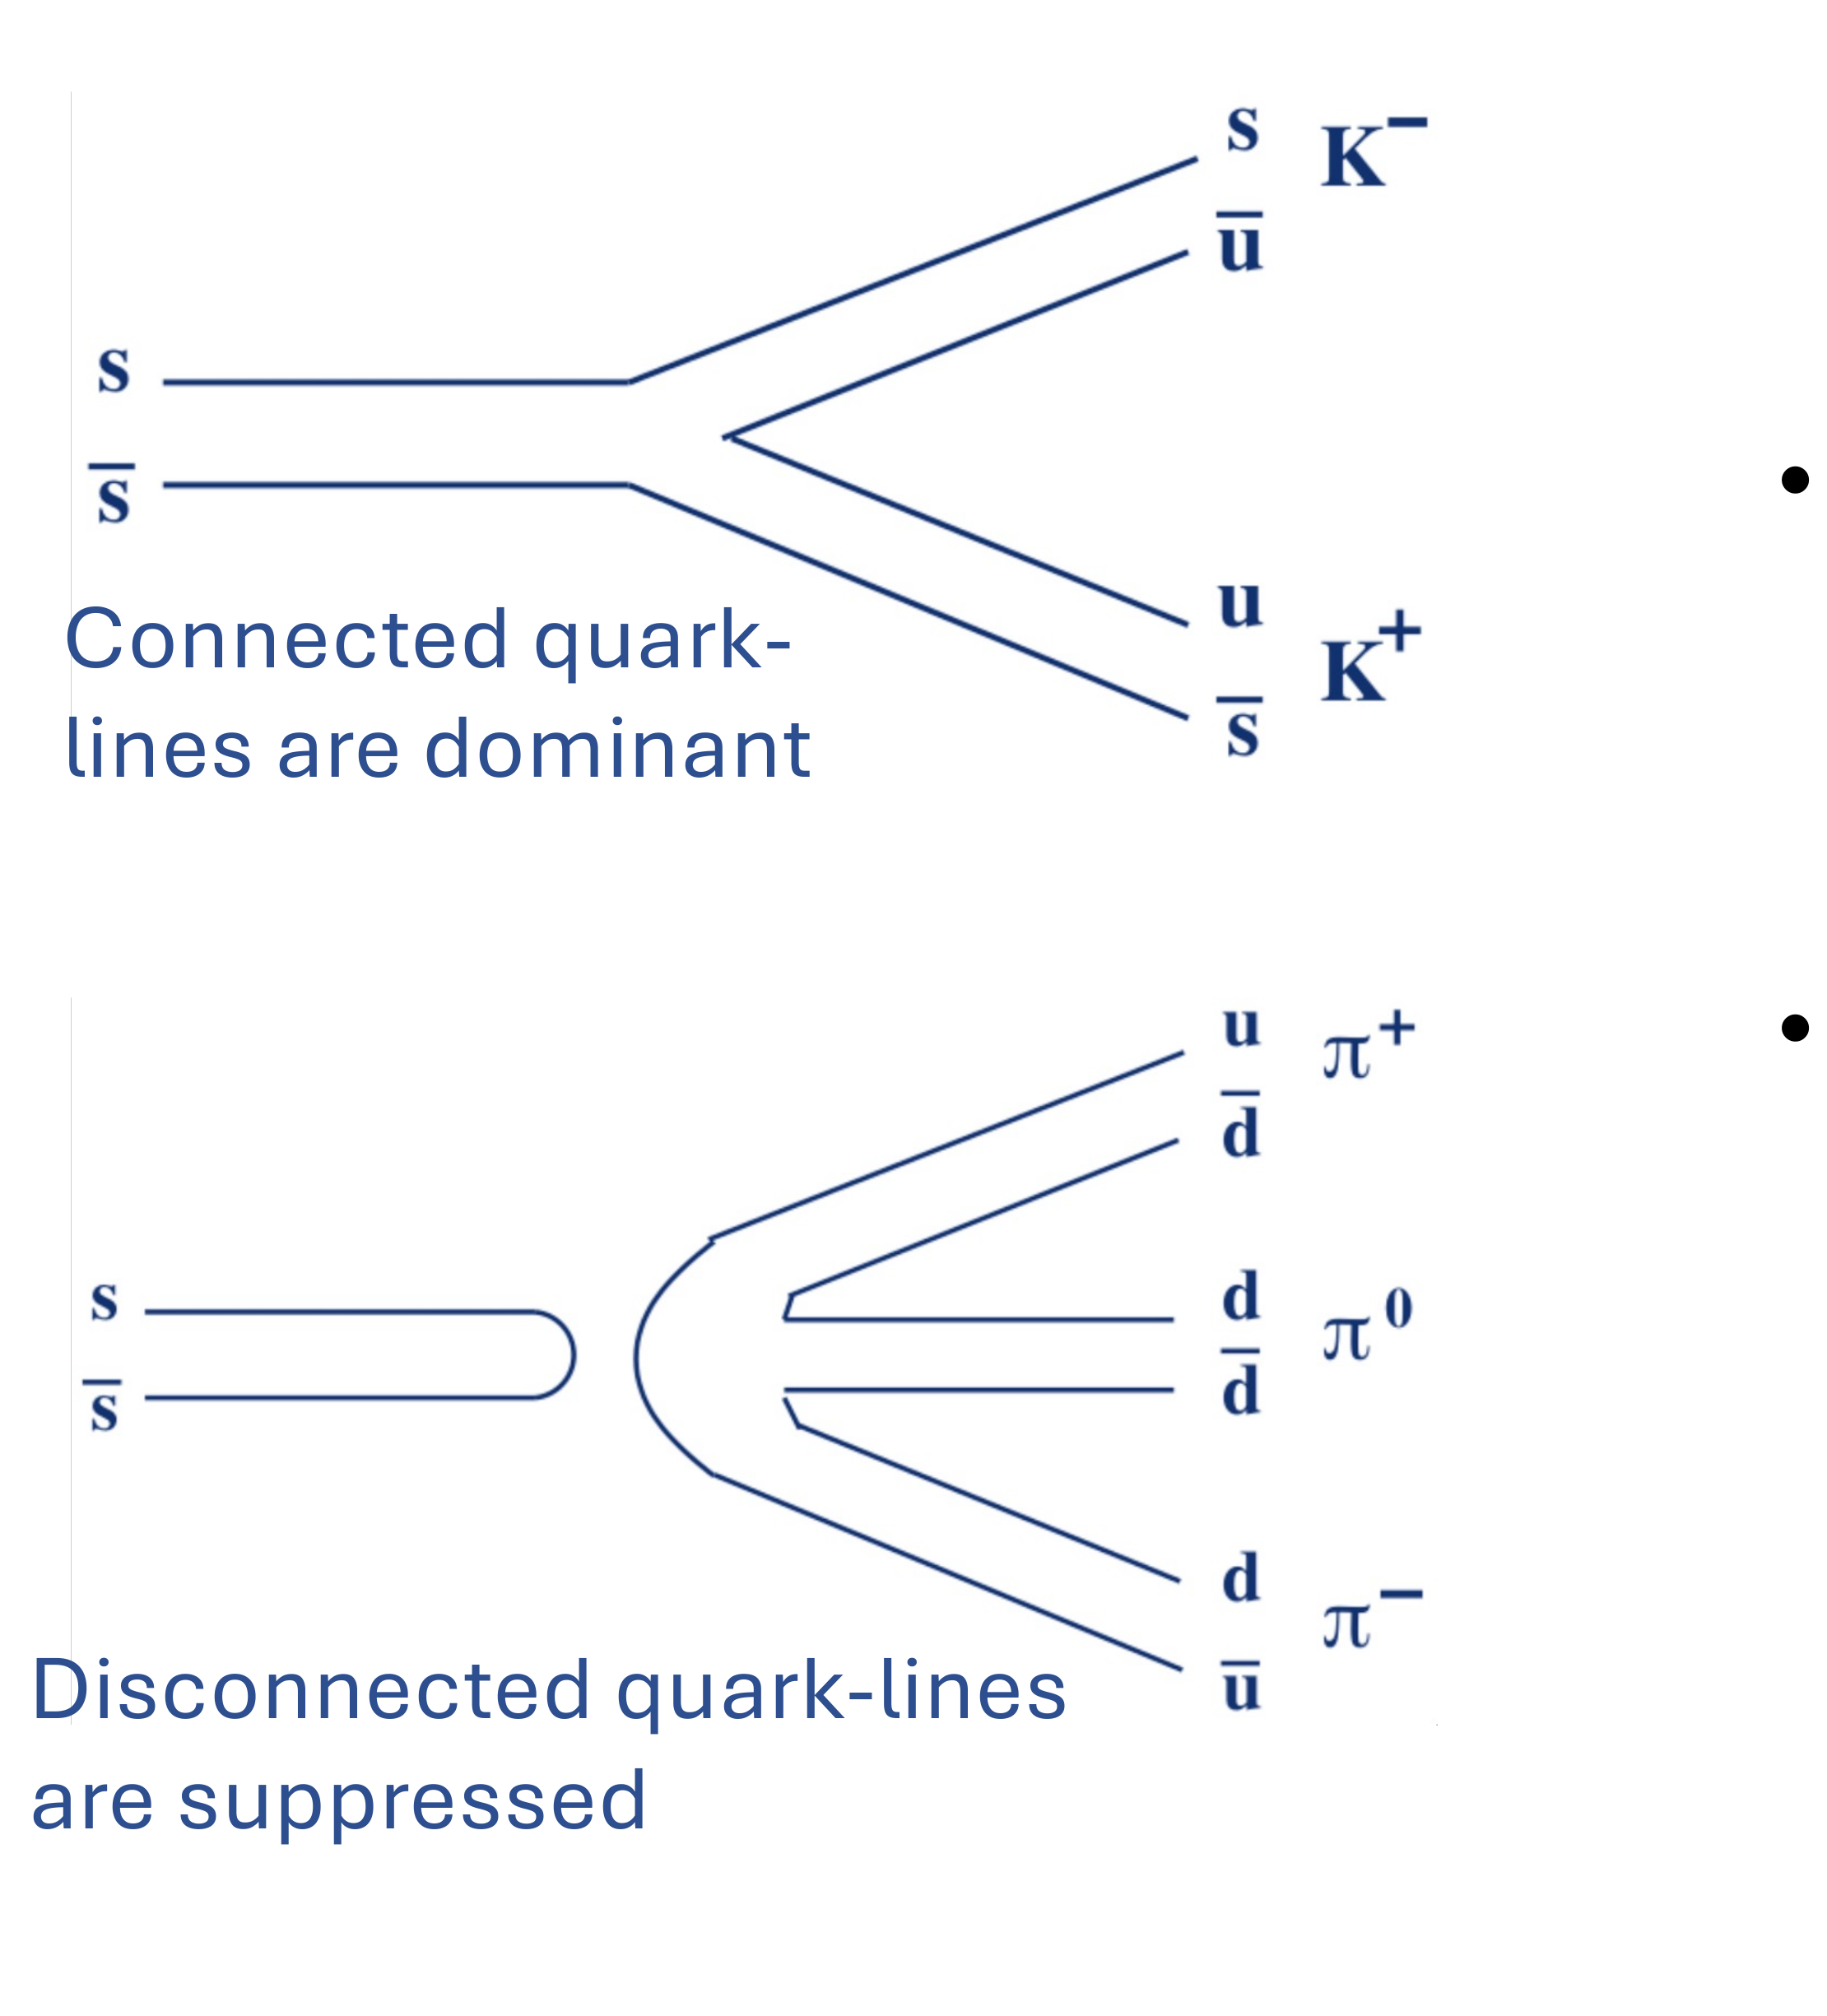
\includegraphics[width=0.55\linewidth]{Figures/ozi_phi.png}
    \caption{Quark-line diagrams for $\phi(s\bar s)$ decay. The connected
    $K\bar K$ graph (top) is OZI allowed and dominates, whereas the
    disconnected $3\pi$ graph (bottom), in which the $s\bar s$ pair
    annihilates, is OZI suppressed. Adapted from the lecture slides (week 19,
    "OZI rule").}
    \label{fig:ozi_phi}
\end{figure}

A complementary and more quantitative probe of the quark content is the leptonic
width of the vector mesons, the decay $V \to e^+e^-$ proceeding through a single
virtual photon coupling to the quark charges. The rate is proportional to the square
of the charge-weighted sum of the flavor amplitudes,
\begin{equation}
    \Gamma(V \to e^+e^-) \;\propto\; \Big|\textstyle\sum_q e_q\,c_q\Big|^2,
    \label{eq:leptonic_width}
\end{equation}
where $e_q$ are the quark charges and $c_q$ the wavefunction coefficients. Inserting
the ideally mixed states $\ket{\rho^0} = \tfrac{1}{\sqrt 2}\ket{u\bar u - d\bar d}$,
$\ket{\omega} = \tfrac{1}{\sqrt 2}\ket{u\bar u + d\bar d}$ and
$\ket{\phi} = -\ket{s\bar s}$ with $e_u = +\tfrac{2}{3}$,
$e_d = e_s = -\tfrac{1}{3}$ gives the squared amplitudes $\tfrac12$, $\tfrac{1}{18}$
and $\tfrac19$, that is
\begin{equation}
    \Gamma_\rho : \Gamma_\omega : \Gamma_\phi = 9 : 1 : 2.
    \label{eq:leptonic_ratio}
\end{equation}
The measured widths in Table~\ref{tab:leptonic_widths} reproduce the predicted
hierarchy remarkably well given the crudeness of the single-photon estimate
\cite[Ch.~7]{Amsler2018}. The residual discrepancies, most visibly for the $\rho^0$,
arise from $\rho$--$\omega$ interference: the small $u$--$d$ mass difference breaks
charge symmetry so that the physical $\rho$ and $\omega$ are not pure isospin
eigenstates but each contain a small admixture of the other's isospin, an effect
studied for instance by the Crystal Barrel collaboration in $\bar p p$ annihilation.

\begin{table}[t]
    \centering
    \caption{Leptonic widths $\Gamma_{e^+e^-}$ of the vector mesons compared with
    the quark-charge prediction of Eq.~\eqref{eq:leptonic_width}. Experimental
    values from the PDG; the ratios are normalized to the $\omega$
    \cite[Ch.~7]{Amsler2018}.}
    \label{tab:leptonic_widths}
    \begin{tabular}{lccccc}
        \hline
         & $\rho^0$ & $\omega$ & $\phi$ & $J/\psi$ & $\Upsilon$ \\
        \hline
        $\Gamma_{e^+e^-}$ [keV] &
        $7.04$ & $0.60$ & $1.27$ & $5.53$ & $1.34$ \\
        Measured ratio &
        $\sim\!11.7$ & $\sim\!1$ & $\sim\!2.1$ & $\sim\!9.2$ & $\sim\!2.2$ \\
        Expected ratio &
        $\sim\!9$ & $\sim\!1$ & $\sim\!2$ & $\sim\!8$ & $\sim\!2$ \\
        \hline
    \end{tabular}
\end{table}

% ============================================================
\subsection{Nomenclature of conventional mesons}
\label{subsec:nomenclature}

Before 1986 hadron names were assigned haphazardly, often reflecting the fantasy or
the name of the discoverer; the rapidly growing number of states made a systematic
scheme indispensable. The convention introduced by the Particle Data Group in 1986
assigns names from which the quantum numbers $J^{PC}$ and the isospin can be read off,
while preserving the familiar labels of the long-known states such as the pion, the
kaon and the $\rho$ \cite[Ch.~4]{Amsler2018}. Two complementary labels are used: the
measured $J^{PC}$, and the spectroscopic notation $^{2s+1}L_J$ which encodes the
internal quantum numbers in the non-relativistic quark model.

The base symbol is fixed by the isospin and by the $J^{PC}$ of the neutral,
hidden-flavor member for which $C$ is defined, as summarized in
Table~\ref{tab:meson_naming}. A subscript $J$ is appended for all states except the
pseudoscalars ($0^{-+}$) and the vectors ($1^{--}$), whose ground states keep their
historical names. For example, the $\rho_3(1690)$ is an established orbital
excitation with $L = 2$, quantum numbers $J^{PC} = 3^{--}$ and isospin $I = 1$
\cite[Ch.~4]{Amsler2018}.

\begin{table}[t]
    \centering
    \caption{Naming scheme for the light $q\bar q$ mesons. The base name is set by
    the isospin $I$ and the spin--parity, with the spectroscopic term $^{2s+1}L_J$
    given for reference \cite[Ch.~4]{Amsler2018}.}
    \label{tab:meson_naming}
    \begin{tabular}{cccccccc}
        \hline
        $L$ & $s$ & $J^{PC}$ & $^{2s+1}L_J$ &
        $I = 1$ & $I = 0$ & $I = 0$ & strange \\
        \hline
        $0$ & $0$ & $0^{-+}$ & $^1S_0$ & $\pi$ & $\eta$  & $\eta'$ & $K$    \\
        $0$ & $1$ & $1^{--}$ & $^3S_1$ & $\rho$ & $\omega$ & $\phi$ & $K^*$  \\
        $1$ & $0$ & $1^{+-}$ & $^1P_1$ & $b_1$ & $h_1$   & $h_1'$  & $K_1$  \\
        $1$ & $1$ & $0^{++}$ & $^3P_0$ & $a_0$ & $f_0$   & $f_0'$  & $K_0^*$\\
        $1$ & $1$ & $1^{++}$ & $^3P_1$ & $a_1$ & $f_1$   & $f_1'$  & $K_1$  \\
        $1$ & $1$ & $2^{++}$ & $^3P_2$ & $a_2$ & $f_2$   & $f_2'$  & $K_2^*$\\
        \hline
    \end{tabular}
\end{table}

\begin{figure}[htbp]
    \centering
    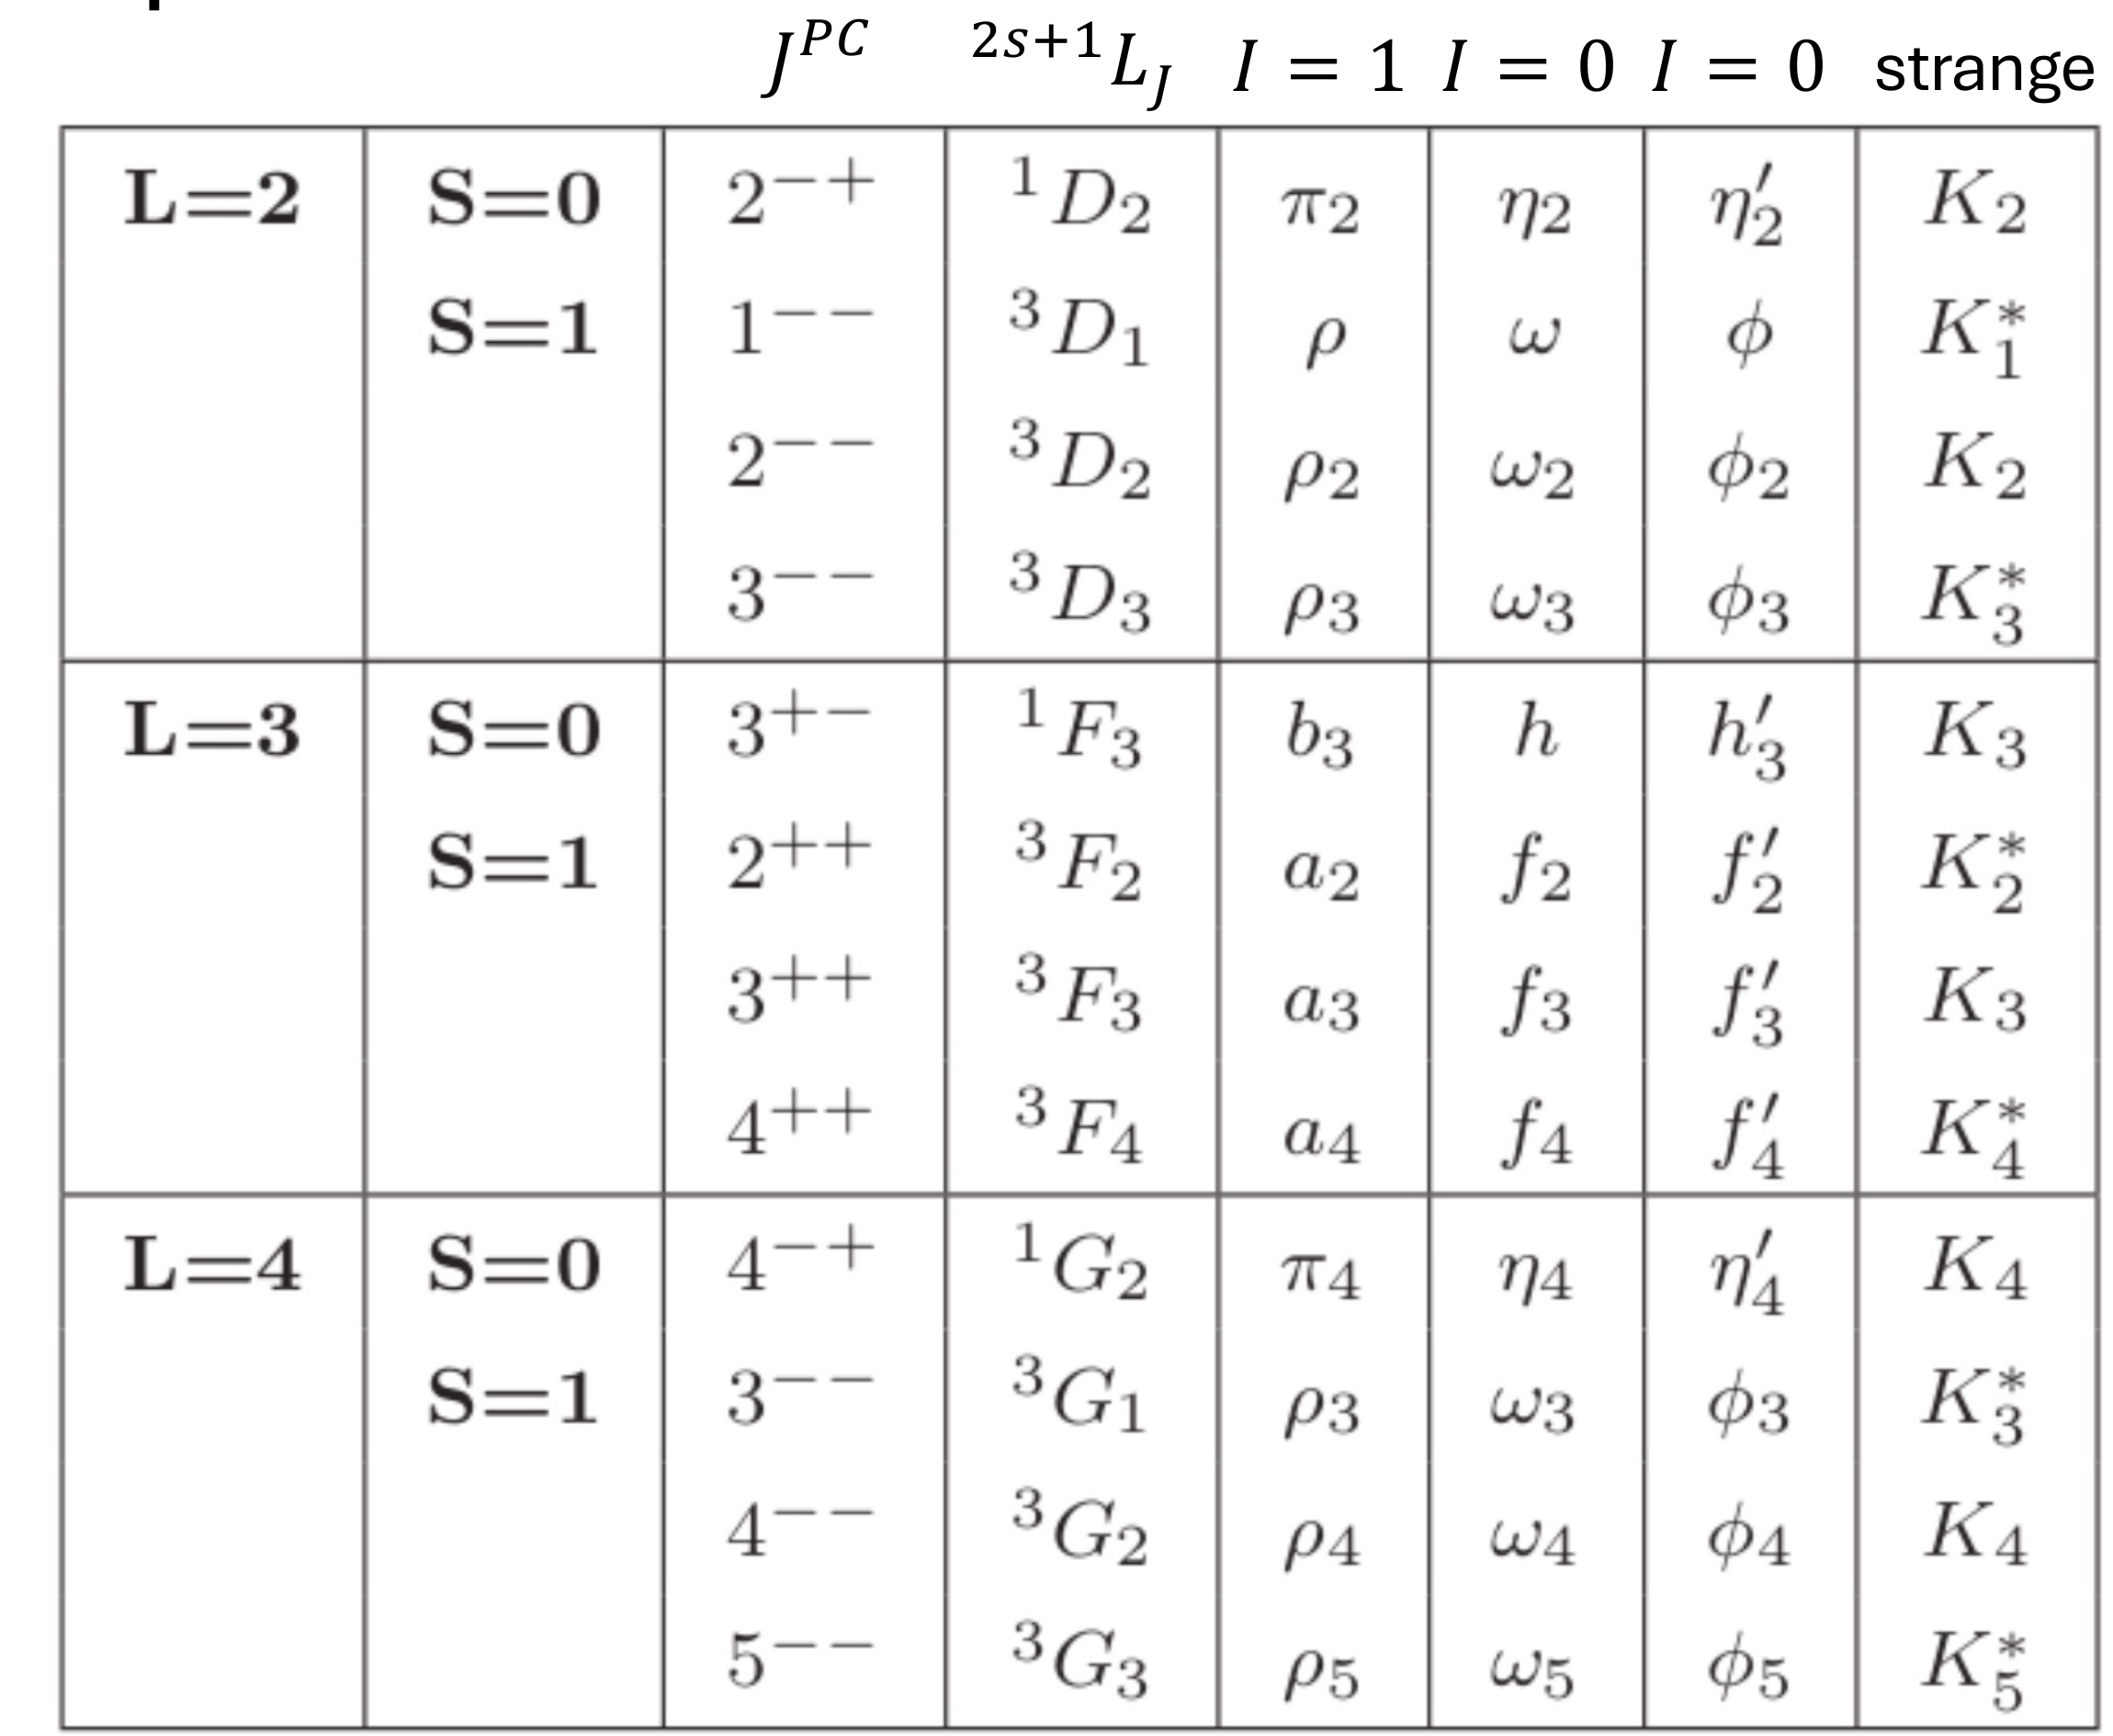
\includegraphics[width=0.65\linewidth]{Figures/meson_naming_extended.png}
    \caption{Continuation of the naming scheme for $L=2,3,4$ ($D$-, $F$- and
    $G$-wave mesons). Adapted from the lecture slides (week 19, "Conventional
    mesons: Naming scheme").}
    \label{fig:meson_naming_extended}
\end{figure}

% ============================================================
\subsection{The \texorpdfstring{$\eta$}{eta} meson as a gateway to QCD and new physics}
\label{subsec:eta-gateway}

The $\eta$ occupies a special place among the light mesons. With a mass of
$m(\eta) = 548$~MeV it has ample phase space to decay into pions, yet its quantum
numbers $I^{G}(J^{PC}) = 0^+ 0^{-+}$ forbid or suppress the most obvious channels,
turning the particle into a sensitive testing ground for the symmetries of the strong
interaction \cite[Ch.~3]{Amsler2018}. The two-pion mode is forbidden outright: with
$J_\eta = 0$ the pions must be in a relative $S$ wave, giving the pair the parity
$P(\pi\pi) = (-1)^L\,P(\pi)^2 = +1$, in conflict with the negative parity of the
$\eta$. The three-pion mode respects parity but violates $G$ parity, since
$G(\eta) = +1$ while $G(3\pi) = (-1)^3 = -1$; equivalently, three isospin-$1$ pions
cannot be coupled to the isospin-$0$ of the $\eta$ in a fully symmetric way, so the
decay is forbidden by isospin symmetry. Nevertheless it is observed with a sizeable
branching ratio, $BR(\eta\to3\pi)\approx 55\%$ \cite[Ch.~3]{Amsler2018}.

The resolution is that isospin is not an exact symmetry: because $m_u \neq m_d$, the
$\pi^0$ and the $\eta$ mix,
\begin{equation}
    \ket{\eta_{\text{phys}}} = \ket{\eta} - \epsilon\,\ket{\pi^0},
    \qquad
    \epsilon \sim (m_d - m_u),
    \label{eq:pi_eta_mixing}
\end{equation}
so that the physical $\eta$ decays ``through'' its small $\pi^0$ admixture. The rate
of $\eta\to3\pi$ is therefore directly sensitive to the light-quark mass difference,
making the $\eta$ a precision laboratory for one of the fundamental parameters of
QCD \cite[Ch.~3]{Amsler2018}.

The same suppression of conventional channels makes the $\eta$ attractive as a
window onto physics beyond the Standard Model. With many of its strong and
electromagnetic decays forbidden or strongly suppressed, the relative weight of any
rare or symmetry-violating mode is enhanced. The rare radiative decay
$\eta \to \pi\gamma\gamma$, in particular, can be used to search for light, weakly
coupled mediators over a broad mass range: a new boson produced in
$\eta \to B'\gamma \to \pi^0\gamma\gamma$ or a light scalar in
$\eta \to \pi^0 S \to \pi^0\gamma\gamma$ would appear as a peak in the
$\pi^0\gamma$ (or diphoton) invariant-mass spectrum on top of the Standard-Model
continuum.

\begin{figure}[htbp]
    \centering
    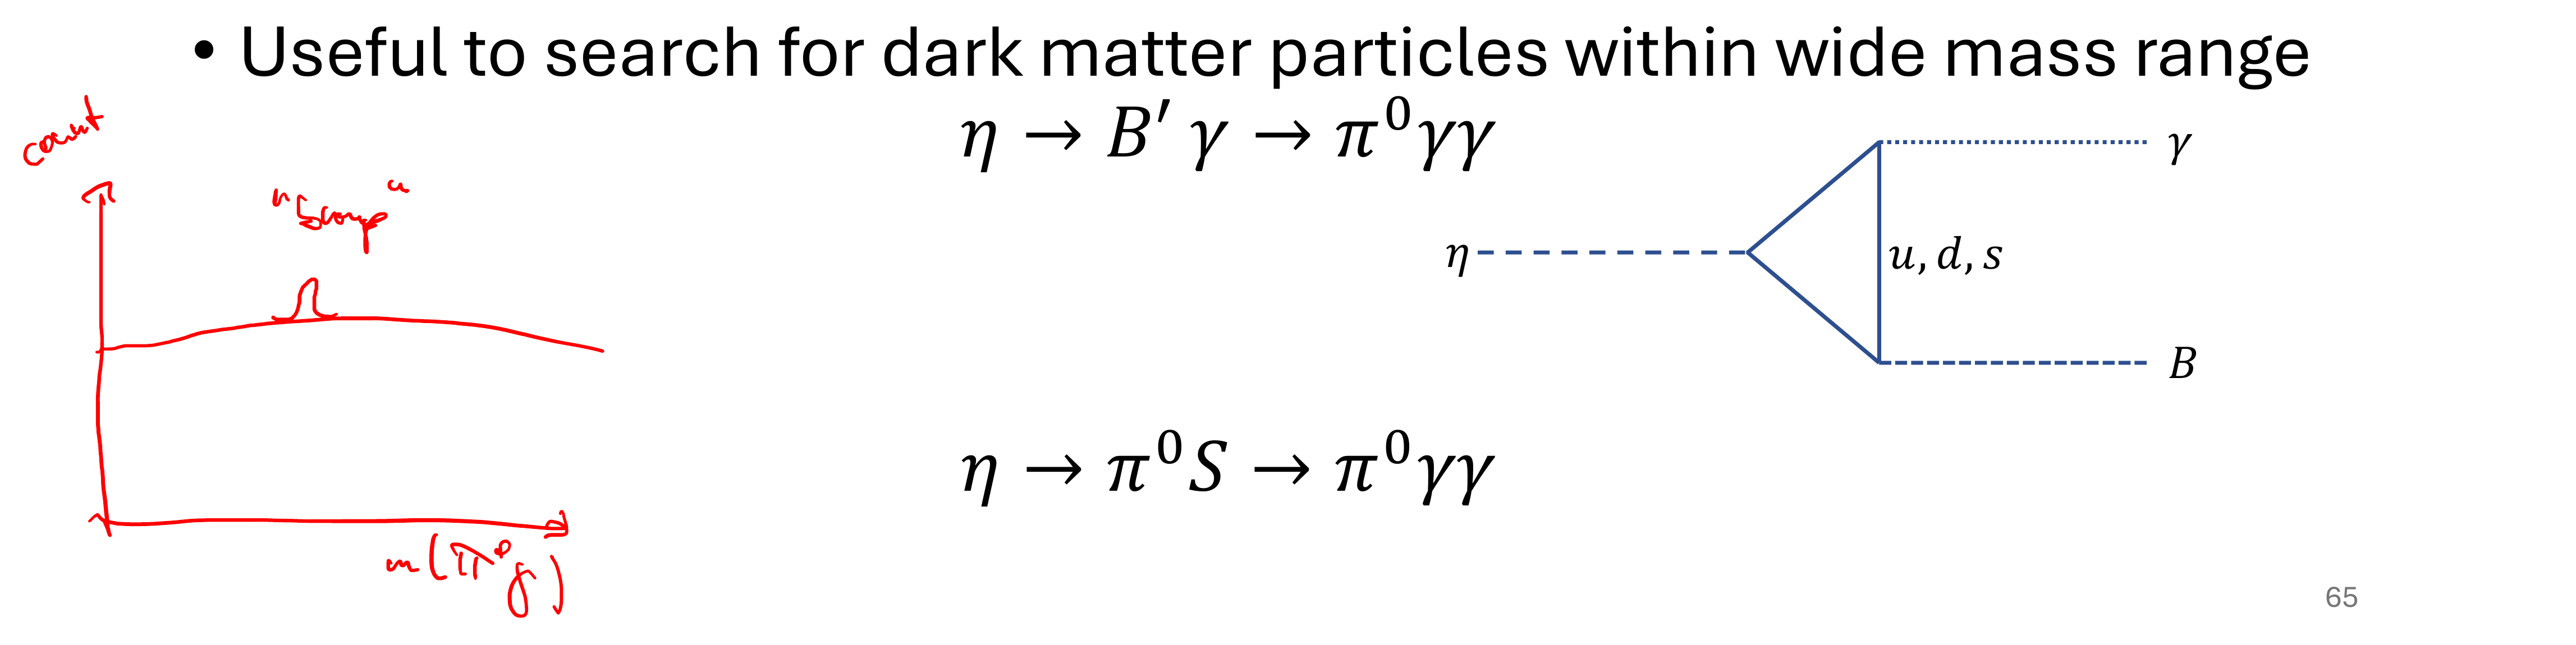
\includegraphics[width=0.85\linewidth]{Figures/eta_rare_decay.png}
    \caption{Quark-loop diagram for the rare decay
    $\eta\to\pi^0\gamma\gamma$ (via a $u,d,s$ triangle loop) and its
    new-physics variants $\eta\to B'\gamma\to\pi^0\gamma\gamma$ and
    $\eta\to\pi^0 S\to\pi^0\gamma\gamma$, together with a sketch of the
    expected $\pi^0\gamma$ invariant-mass spectrum: a hypothetical light
    mediator would appear as a narrow ``bump'' over the Standard-Model
    continuum. Adapted from the lecture slides (week 19, "The eta meson as
    gate to new physics").}
    \label{fig:eta_rare_decay}
\end{figure}
\section{Baryons and color}
\label{sec:baryons-color}

% ============================================================
\subsection{Baryon wavefunction and the antisymmetry problem}
\label{subsec:baryon-antisymmetry}

Baryons are bound states of three quarks, and since quarks are spin-$\tfrac{1}{2}$
fermions the Pauli principle requires the total wavefunction to be antisymmetric
under the exchange of any pair of constituents. In the non-relativistic quark model
the wavefunction factorizes into a flavor part, a spin part and a spatial part,
\begin{equation}
    \psi = \Phi_{\text{flavor}}\,\chi_{\text{spin}}\,R(\vec{r}),
    \label{eq:baryon-Psi-nocolor}
\end{equation}
which is the form available before color is introduced \cite[Ch.~13]{Amsler2018}.
The spatial factor of the ground-state baryons carries no orbital angular momentum,
$L = 0$, and is therefore symmetric, so the required antisymmetry has to be supplied
by the combined flavor and spin factors alone.

The building blocks are fixed by the group-theoretical decompositions of three
fundamental representations. For flavor one finds
\begin{equation}
    \mathbf{3} \otimes \mathbf{3} \otimes \mathbf{3}
    = \mathbf{10}_{S} \oplus \mathbf{8}_{MS} \oplus \mathbf{8}_{MA}
      \oplus \mathbf{1}_{A},
    \label{eq:flavor-3x3x3}
\end{equation}
giving a totally symmetric decuplet, two octets of mixed symmetry and a totally
antisymmetric singlet \cite[Ch.~13]{Amsler2018}. For the three quark spins the
analogous coupling reads
\begin{equation}
    \mathbf{2} \otimes \mathbf{2} \otimes \mathbf{2}
    = \mathbf{4}_{S} \oplus \mathbf{2}_{MS} \oplus \mathbf{2}_{MA},
    \label{eq:spin-2x2x2}
\end{equation}
that is, one fully symmetric spin-$\tfrac{3}{2}$ quadruplet and two spin-$\tfrac{1}{2}$
doublets of mixed symmetry. Note that no totally antisymmetric combination of three
spin-$\tfrac{1}{2}$ states exists, a fact that will prove decisive below.

Experimentally the baryons of lowest mass arrange themselves into exactly the
multiplets that these representations predict: a spin-$\tfrac{1}{2}$ octet containing
the proton and the neutron, and a spin-$\tfrac{3}{2}$ decuplet containing the
$\Delta(1232)$. Both are observed as the ground states, with $L = 0$ and hence a
symmetric spatial wavefunction \cite[Ch.~13]{Amsler2018}.

The difficulty becomes most transparent at the corners of the decuplet, where the
three quark flavors are identical. The state
\begin{equation}
    \Delta^{++} = \ket{uuu}\,\ket{\uparrow\uparrow\uparrow}\,\ket{L=0}
\end{equation}
is symmetric in flavor, symmetric in spin and symmetric in space, so the product
\eqref{eq:baryon-Psi-nocolor} is \emph{totally symmetric} under quark exchange. The
same holds for the $\Delta^-(ddd)$ and the $\Omega^-(sss)$. Such configurations
manifestly violate the Pauli principle for identical fermions, and with only the
factors in \eqref{eq:baryon-Psi-nocolor} at hand there is no way to repair the
symmetry \cite[Ch.~10]{Amsler2018}. The quark model, otherwise so successful in
accounting for the observed multiplets, is thereby driven into a genuine
contradiction whose resolution requires an additional degree of freedom.

\begin{figure}[htbp]
  \centering
  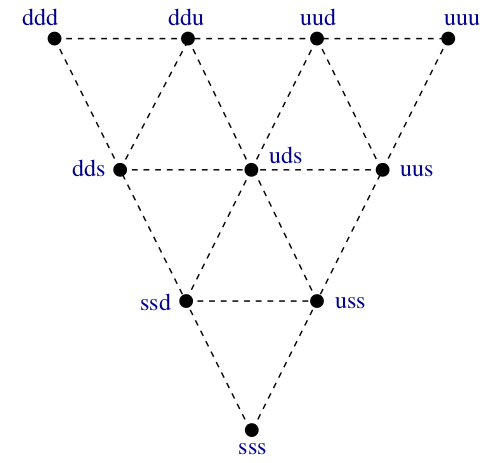
\includegraphics[width=0.55\textwidth]{Figures/decuplet_corners.png}
  \caption{Weight diagram of the spin-$\tfrac{3}{2}$ baryon decuplet. The three
  corner states $\Delta^{++}(uuu)$, $\Delta^-(ddd)$ and $\Omega^-(sss)$ are built
  from three identical quarks with aligned spins and a symmetric $L=0$ spatial
  wavefunction, and are therefore totally symmetric under exchange. Adapted
  from the lecture slides (week 19, "Baryons in SU(6)").}
  \label{fig:decuplet-corners}
\end{figure}

\FloatBarrier

% ============================================================
\subsection{Baryons in SU(6) and the ``56''-plet}
\label{subsec:su6-56plet}

The flavor and spin degrees of freedom can be combined into a single larger symmetry
by embedding the three flavors and the two spin states into a sixfold fundamental
representation. Coupling three such sextets and reducing the product with the help of
Young tableaux gives
\begin{equation}
    \mathbf{6} \otimes \mathbf{6} \otimes \mathbf{6}
    = \mathbf{56}_{S} \oplus \mathbf{70}_{MS} \oplus \mathbf{70}_{MA}
      \oplus \mathbf{20}_{A},
    \label{eq:su6-6x6x6}
\end{equation}
where the subscripts again record the permutation symmetry \cite[Ch.~13]{Amsler2018}.
Each $\mathrm{SU}(6)$ supermultiplet decomposes into definite combinations of an
$\mathrm{SU}(3)$ flavor multiplet and a definite total quark spin. The totally
symmetric $\mathbf{56}$ contains precisely the observed ground states,
\begin{equation}
    \mathbf{56} = (\mathbf{8},\, s=\tfrac{1}{2}) \;\oplus\; (\mathbf{10},\, s=\tfrac{3}{2}),
\end{equation}
that is, the spin-$\tfrac{1}{2}$ octet of nucleons and the spin-$\tfrac{3}{2}$
decuplet headed by the $\Delta(1232)$ \cite[Ch.~13]{Amsler2018}. The ground-state
baryons therefore fit the ``56''-plet without exception, which at first sight is a
remarkable success of the scheme.

The flavor wavefunctions that enter these assignments illustrate how the symmetry is
realized. For the $\Delta$ the totally symmetric flavor function is
\begin{equation}
    \Phi_{\Delta} = \sqrt{\tfrac{1}{3}}
    \big[\, uud + (ud + du)u \,\big],
\end{equation}
while the two mixed-symmetry partners needed for the octet read
\begin{equation}
    \Phi_{MA} = \sqrt{\tfrac{1}{2}}\,\big[\,(ud - du)u\,\big],
    \qquad
    \Phi_{MS} = \sqrt{\tfrac{1}{6}}\,\big[\,(ud + du)u - 2\,uud\,\big].
\end{equation}
A totally symmetric spin-$\tfrac{1}{2}$ wavefunction is then assembled from the
mixed-symmetric and mixed-antisymmetric flavor and spin factors, the proton being the
symmetric combination $\tfrac{1}{\sqrt{2}}\,(\Phi_{MS}\chi_{MS}
+ \Phi_{MA}\chi_{MA})$ \cite[Ch.~13]{Amsler2018}.

This is exactly where the antisymmetry problem of Sect.~\ref{subsec:baryon-antisymmetry}
returns in its sharpest form. The $\mathbf{56}$ is totally symmetric in the combined
flavor--spin variables, and for the ground states the orbital wavefunction $R(\vec r)$
with $L=0$ is symmetric as well. The product
\begin{equation}
    \Psi^{\text{total}} = \Phi_{\text{flavor}}\,\chi_{\text{spin}}\,R(\vec{r})
\end{equation}
is then symmetric, in direct conflict with the Pauli principle, which demands a
totally antisymmetric baryon. The very multiplet that accommodates all the observed
ground states is the one with the wrong overall symmetry, so the success of the
classification and its apparent failure under fermion statistics are two sides of the
same fact \cite[Ch.~13]{Amsler2018}.

\FloatBarrier

% ============================================================
\subsection{Magnetic moments and the constituent quark masses}
\label{subsec:magnetic-moments}

Before turning to color it is worth extracting a quantitative prediction from the
$\mathrm{SU}(6)$ wavefunctions just constructed. The magnetic moments of the ground-state
baryons are among the earliest and most convincing successes of the quark model, and they
provide the standard route to the \emph{constituent} quark masses---the effective masses a
quark acquires inside a hadron, much larger than the bare masses generated by the Higgs
mechanism.

Treating the quarks as point-like Dirac fermions with $g = 2$, each carries a magnetic
moment $\mu_i = Q_i e / 2 m_i$ aligned with its spin. The moment of a baryon is the
expectation value of the sum of the three quark moments in the state with maximal spin
projection,
\begin{equation}
    \mu_B = \frac{e}{2 m_q}
    \bra{B} \sum_{i=1}^{3} Q_i \,\sigma_{3}(i) \ket{B},
    \label{eq:magnetic-moment-operator}
\end{equation}
where $Q_i$ is the quark charge in units of $e$, $\sigma_3(i)$ acts on the spin of the
$i$-th quark, and $m_q = m_u = m_d$ in the isospin-symmetric limit
\cite[Ch.~15]{Amsler2018}.

\paragraph{Worked example: the neutron and the light constituent mass.}
The neutron is the $udd$ member of the octet, with the spin--flavor wavefunction obtained
from the proton one by $u \leftrightarrow d$. Written out for spin projection
$+\tfrac{1}{2}$, the totally symmetric combination gives, for each quark, a probability
$\tfrac{1}{3}$ of carrying spin antiparallel to the baryon and $\tfrac{2}{3}$ parallel,
weighted so that the expectation value of $\sigma_3$ is $-\tfrac{1}{3}$ for the two
like-flavor quarks and $+\tfrac{4}{3}$ for the odd one. Evaluating
Eq.~\eqref{eq:magnetic-moment-operator} on the octet wavefunctions gives, for the two
members of the nucleon doublet,
\begin{equation}
    \mu_p = \frac{4}{3}\,\mu_u - \frac{1}{3}\,\mu_d ,
    \qquad
    \mu_n = \frac{4}{3}\,\mu_d - \frac{1}{3}\,\mu_u ,
    \label{eq:mu-n-setup}
\end{equation}
the odd-flavor quark entering with weight $-\tfrac13$ and the like-flavor pair with
$+\tfrac43$. Inserting $\mu_u = \tfrac{2}{3}\,e/2m_q$ and $\mu_d = -\tfrac{1}{3}\,e/2m_q$,
\begin{equation}
    \mu_n = \left(-\frac{4}{9} - \frac{2}{9}\right)\frac{e}{2m_q}
          = -\,\frac{e}{3 m_q},
    \qquad
    \mu_p = \left(\frac{8}{9} + \frac{1}{9}\right)\frac{e}{2m_q}
          = +\,\frac{e}{2 m_q}.
    \label{eq:mu-n}
\end{equation}
The model therefore
predicts the ratio
\begin{equation}
    \frac{\mu_p}{\mu_n} = -\frac{3}{2},
    \label{eq:mu-ratio}
\end{equation}
against the measured $\mu_p/\mu_n = 2.793/(-1.913) = -1.46$---a parameter-free prediction accurate to a few percent, and
historically one of the strongest arguments that the quarks are real dynamical objects
rather than a bookkeeping device.

Equation~\eqref{eq:mu-n} can be read backwards. Inserting the measured neutron moment
$\mu_n = -1.913\,\mu_N$, with the nuclear magneton $\mu_N = e/2M_p$, gives
\begin{equation}
    m_q = \frac{2 M_p}{3 \times 1.913} \;\approx\; 327\;\mathrm{MeV},
    \label{eq:mq-from-mun}
\end{equation}
close to the value $m_u \simeq m_d \simeq 350\;\mathrm{MeV}$ usually quoted for the light
constituent masses. Amsler runs the same inversion through the \emph{proton} instead,
$\mu_p = 2.79\,\mu_N = e/2m$, obtaining $m = M_p/2.79 = 336\;\mathrm{MeV}$
\cite[Ch.~14]{Amsler2018}; the small difference between the two routes is a measure of how
far the model is from exact. The same calculation is carried out by Halzen and Martin
\cite[Ch.~2]{HalzenMartin1984} and by Perkins \cite[Ch.~4]{Perkins2000}.

\paragraph{Worked example: the strange quark mass from the $\Lambda$.}
The $\Lambda$ is especially clean. Its $ud$ pair is coupled to isospin $I=0$ and hence,
by the symmetry of the octet wavefunction, to spin $s=0$; the two light quarks therefore
contribute nothing to the moment, and the entire spin of the $\Lambda$ is carried by the
strange quark. Consequently
\begin{equation}
    \mu_\Lambda = \mu_s = \frac{Q_s e}{2 m_s} = -\,\frac{e}{6 m_s}.
    \label{eq:mu-lambda}
\end{equation}
With the measured $\mu_\Lambda = -0.613\,\mu_N$ this yields
\begin{equation}
    m_s = \frac{M_p}{3 \times 0.613} \;\approx\; 510\;\mathrm{MeV},
    \label{eq:ms-from-mulambda}
\end{equation}
in good agreement with the constituent value $m_s \simeq 500\;\mathrm{MeV}$. Amsler's
treatment of the hyperon moments proceeds identically, deducing the vanishing $ud$
contribution from $I(ud) = 0$ and hence $s(ud) = 0$ \cite[Ch.~14]{Amsler2018}. The difference
$m_s - m_q \approx 180\;\mathrm{MeV}$ is of the same order as the $130$--$150\;\mathrm{MeV}$
per unit of strangeness that governs the equal-spacing rule of Sect.~\ref{subsec:gmo}. Constituent masses obtained this
way are collected in Appendix~\ref{app:useful-tables}.

\FloatBarrier

% ============================================================
\subsection{Color as a new degree of freedom}
\label{subsec:color-dof}

The resolution, proposed in the mid-1960s by Greenberg and by Han and Nambu, and
developed by Gell-Mann, is to endow each quark flavor with a further internal quantum
number called \emph{color} \cite[Ch.~10]{Amsler2018}. Every quark comes in three
color states, labeled red ($r$), green ($g$) and blue ($b$), which span the
fundamental triplet of a new symmetry group $\mathrm{SU}(3)_{c}$. Unlike flavor
$\mathrm{SU}(3)$, which is badly broken by the quark mass differences, the color
symmetry $\mathrm{SU}(3)_{c}$ is taken to be exact.

The color states couple in the same way as the flavors,
\begin{equation}
    \mathbf{3} \otimes \mathbf{3} \otimes \mathbf{3}
    = \mathbf{10}_{S} \oplus \mathbf{8}_{MS} \oplus \mathbf{8}_{MA}
      \oplus \mathbf{1}_{A},
\end{equation}
and it is the totally antisymmetric singlet $\mathbf{1}_{A}$ that is used to restore
the overall antisymmetry of the baryon \cite[Ch.~10]{Amsler2018}. Explicitly, the
antisymmetric color wavefunction of three quarks is
\begin{equation}
\begin{split}
    \lambda_{\text{color}}(q_1 q_2 q_3) = \frac{1}{\sqrt{6}}
    \big[\, & q_1(r)q_2(g)q_3(b) + q_1(b)q_2(r)q_3(g) + q_1(g)q_2(b)q_3(r) \\
    & - q_1(g)q_2(r)q_3(b) - q_1(b)q_2(g)q_3(r) - q_1(r)q_2(b)q_3(g) \,\big].
\end{split}
\end{equation}
Multiplying the symmetric flavor--spin--space wavefunction of the ``56''-plet by this
antisymmetric color factor yields a total wavefunction
\begin{equation}
    \psi = \Phi_{\text{flavor}}\,\chi_{\text{spin}}\,\lambda_{\text{color}}\,R(\vec{r}),
    \label{eq:full-Psi-color}
\end{equation}
in which the symmetric product $\Phi_{\text{flavor}}\,\chi_{\text{spin}}\,R(\vec{r})$
is multiplied by the antisymmetric $\lambda_{\text{color}}$, so that the result is
antisymmetric and the Pauli principle is satisfied \cite[Ch.~10]{Amsler2018}. The
$\Delta^{++}$, $\Delta^-$ and $\Omega^-$ are thereby rescued precisely because their
color factor carries the antisymmetry that the rest of the wavefunction lacks.

A baryon built from the color singlet is colorless, or ``white''. This is the
quantitative content of the observation that all hadrons seen in nature are color
singlets: color charge itself is never observed in isolation, and only color-neutral
combinations propagate as free particles \cite[Ch.~10]{Amsler2018}. The exactness of
$\mathrm{SU}(3)_{c}$ together with this confinement of color provides the foundation on which Quantum Chromodynamics is built.

\FloatBarrier

% ============================================================
\subsection{Gluons and the color octet}
\label{subsec:gluons-octet}

If color is to be a dynamical charge, the force between quarks must transmit it. The
mediators of the strong interaction, the gluons, therefore carry one unit of color and
one unit of anticolor, color being conserved at each quark--gluon vertex
\cite[Ch.~10]{Amsler2018}. The nine combinations of a color with an anticolor reduce
in the same manner as the $q\bar q$ mesons,
\begin{equation}
    \mathbf{3} \otimes \overline{\mathbf{3}} = \mathbf{1} \oplus \mathbf{8},
\end{equation}
splitting the color--anticolor states into a singlet and an octet. The eight octet
states,
\begin{equation}
    r\bar g,\; r\bar b,\; g\bar r,\; g\bar b,\; b\bar r,\; b\bar g,\;
    \tfrac{1}{\sqrt{2}}(r\bar r - g\bar g),\;
    \tfrac{1}{\sqrt{6}}(r\bar r + g\bar g - 2 b\bar b),
\end{equation}
are the eight physical gluons, the gauge fields of QCD, while the remaining colorless
combination is the singlet
\begin{equation}
    \tfrac{1}{\sqrt{3}}\,(r\bar r + g\bar g + b\bar b).
\end{equation}

The singlet gluon is not realized in nature, and confinement provides the reason. A
color-singlet gluon would itself be colorless, and a colorless mediator could be
emitted as a free particle and exchanged between two color-singlet hadrons, giving rise
to a long-range strong force with strong coupling \cite[Ch.~10]{Amsler2018}. No such
force is observed, so the singlet does not appear as a physical field and exactly eight
colored gluons remain. Because the gluons carry color themselves, they interact with one
another, a non-Abelian feature that distinguishes QCD from electrodynamics and underlies
both confinement and asymptotic freedom.

\FloatBarrier

% ============================================================
\subsection{Baryon supermultiplets and excited states}
\label{subsec:supermultiplets}

With the total wavefunction antisymmetrized by color as in \eqref{eq:full-Psi-color},
the requirement of antisymmetry can be reformulated for the visible degrees of freedom:
since $\lambda_{\text{color}}$ is always the antisymmetric singlet, the remaining product
$\Phi_{\text{flavor}}\,\chi_{\text{spin}}\,R(\vec{r})$ must be totally
\emph{symmetric}. For the ground states the orbital factor is symmetric and this selects
the ``56''-plet. The excited baryons, however, may carry orbital angular momentum, which
opens additional possibilities for the spatial wavefunction $R(\vec{r})$ and hence for the
$\mathrm{SU}(6)$ content \cite[Ch.~15]{Amsler2018}.

The internal motion of three quarks is conveniently described by the two Jacobi
coordinates
\begin{equation}
    \vec{\rho} = \tfrac{1}{\sqrt{2}}\,(\vec{x}_1 - \vec{x}_2),
    \qquad
    \vec{\lambda} = \tfrac{1}{\sqrt{6}}\,(\vec{x}_1 + \vec{x}_2 - 2\,\vec{x}_3),
\end{equation}
where $\vec{\rho}$ describes the relative motion within a quark pair and $\vec{\lambda}$
the motion of the third quark relative to that pair. The associated orbital angular
momenta determine the parity,
\begin{equation}
    P(qqq) = (-1)^{L_{\rho}}\,(-1)^{L_{\lambda}},
\end{equation}
so that ground-state baryons with $L_{\rho} = L_{\lambda} = 0$ have $J^P =
\tfrac{1}{2}^+$ or $\tfrac{3}{2}^+$ \cite[Ch.~13]{Amsler2018}. In the harmonic-oscillator
model the excitations are organized by the band number
\begin{equation}
    N = 2n + L = 2 n_\rho + 2 n_\lambda + L_{\rho} + L_{\lambda},
\end{equation}
and the spectrum is classified under the combined $\mathrm{SU}(6) \times O(3)$ symmetry,
each level being labeled by an $\mathrm{SU}(6)$ multiplet and its orbital angular momentum $L$ \cite[Ch.~15]{Amsler2018}.

The mixed-symmetry and antisymmetric $\mathrm{SU}(6)$ multiplets, which cannot describe
the symmetric ground states, become accessible once the orbital wavefunction itself
carries a definite mixed or antisymmetric character. The $\vec{\rho}$ excitation is
antisymmetric and the $\vec{\lambda}$ excitation symmetric under exchange of the first two
quarks, and combining these with mixed flavor--spin functions produces a totally symmetric
product. In this way the $\mathbf{70}$-plet appears as the lowest negative-parity band
($N=1$, $L=1$), decomposing into a spin-$\tfrac{3}{2}$ octet together with a decuplet, an
octet and a singlet of spin $\tfrac{1}{2}$, while the totally antisymmetric flavor singlet
$\Phi_A$, which has no place among the ground states, is realized only in these excited
multiplets, namely in the $\mathbf{70}$ and the $\mathbf{20}$
\cite[Ch.~15]{Amsler2018}. The $\mathrm{SU}(6)$ supermultiplets thus organize as
\begin{align}
    \mathbf{56}: &\quad s=\tfrac{1}{2}\ \text{octet},\;\; s=\tfrac{3}{2}\ \text{decuplet}, \nonumber\\
    \mathbf{70}: &\quad s=\tfrac{1}{2}\ \text{decuplet},\;\; s=\tfrac{3}{2}\ \text{octet},\;\;
                   s=\tfrac{1}{2}\ \text{octet},\;\; s=\tfrac{1}{2}\ \text{singlet}, \\
    \mathbf{20}: &\quad s=\tfrac{3}{2}\ \text{singlet},\;\; s=\tfrac{1}{2}\ \text{octet}. \nonumber
\end{align}

These predicted supermultiplets map onto the experimentally established excited baryons.
The known $N^{*}$ and $\Delta^{*}$ resonances, as well as the strange $\Lambda^{*}$ and
$\Sigma^{*}$ states, populate the bands expected from $\mathrm{SU}(6)\times O(3)$, with the
ground-state nucleons and $\Delta(1232)$ in the $(\mathbf{56},0^{+})$ at $N=0$ and the
lowest orbital excitations in the $(\mathbf{70},1^{-})$ at $N=1$
\cite[Ch.~15]{Amsler2018}. The model predicts many more excitations than have been seen;
several states couple only weakly to the pion--nucleon and kaon--nucleon channels used to
produce them, and no firmly established candidate has yet been assigned to the
$\mathbf{20}$-plet \cite[Ch.~15]{Amsler2018}.

The flavor content of the $\mathbf{20}$ has a striking consequence. A totally
\emph{antisymmetric} spatial wavefunction must be paired with the totally antisymmetric
flavor--spin multiplet, which is the $\mathbf{20}$, and the $\mathbf{20}$ contains only a
spin-$\tfrac12$ octet and a spin-$\tfrac32$ singlet---\emph{no decuplet}. Since the
$\Delta$ states live exclusively in flavor decuplets, it follows that a baryon with an
antisymmetric spatial wavefunction can exist as an $N^{*}$ (or $\Lambda^{*}$,
$\Sigma^{*}$, $\Xi^{*}$) but never as a $\Delta^{*}$. This is a clean, falsifiable
prediction of the scheme, and it is part of why the $\mathbf{20}$-plet remains so hard to
identify experimentally: the states it predicts are precisely those that couple most
weakly to the formation channels used to search for them \cite[Ch.~15]{Amsler2018}.

The lowest negative-parity band is the one most thoroughly explored. Combining $L=1$ with
the two spin values available in the $\mathbf{70}$ generates exactly five nucleon states
and two $\Delta$ states, listed in Table~\ref{tab:70-1minus}. The counting follows from
angular-momentum addition alone: for $s=\tfrac12$, $L\otimes s$ gives $J=\tfrac12,
\tfrac32$; for $s=\tfrac32$ it gives $J=\tfrac12,\tfrac32,\tfrac52$; and all carry
$P=-1$. The $\Delta$ sector is restricted to $s=\tfrac12$, because its flavor decuplet is
symmetric and must therefore pair with a mixed-symmetry spin function, so only two
$\Delta^{*}$ states appear.

\begin{table}[htbp]
    \centering
    \caption{The five $N^{*}$ and two $\Delta^{*}$ states of the
    $(\mathbf{70},1^{-})$ band at $N=1$, with their physical assignments.}
    \label{tab:70-1minus}
    \begin{tabular}{llll}
        \hline
        Flavor multiplet & Quark spin $s$ & $J^{P}$ & State \\
        \hline
        octet    & $\tfrac12$ & $\tfrac12^{-}$ & $N(1535)$ \\
        octet    & $\tfrac12$ & $\tfrac32^{-}$ & $N(1520)$ \\
        octet    & $\tfrac32$ & $\tfrac12^{-}$ & $N(1650)$ \\
        octet    & $\tfrac32$ & $\tfrac32^{-}$ & $N(1700)$ \\
        octet    & $\tfrac32$ & $\tfrac52^{-}$ & $N(1675)$ \\
        decuplet & $\tfrac12$ & $\tfrac12^{-}$ & $\Delta(1620)$ \\
        decuplet & $\tfrac12$ & $\tfrac32^{-}$ & $\Delta(1700)$ \\
        \hline
    \end{tabular}
\end{table}

Radial excitations follow the same band-number bookkeeping. Setting $L=0$ but
$n_{\rho}+n_{\lambda}=1$ gives $N=2$ with \emph{positive} parity, since
$P=(-1)^{L_{\rho}+L_{\lambda}}$ depends only on the orbital angular momenta and not on the
radial quantum numbers. A radial excitation therefore carries the same $J^{P}$ as the
state it excites: the first radial excitation of the nucleon is the Roper resonance
$N(1440)\tfrac12^{+}$, and that of the $\Delta(1232)$ is the $\Delta(1600)\tfrac32^{+}$.
The Roper's anomalously low mass---below the negative-parity $N(1535)$, contrary to the
naive oscillator ordering---is a long-standing puzzle discussed in
Sect.~\ref{subsec:transition-ff}. The band structure and the assignments of this section
follow Amsler's treatment of the light baryon excitations \cite[Ch.~15]{Amsler2018}.

\begin{figure}[htbp]
  \centering
  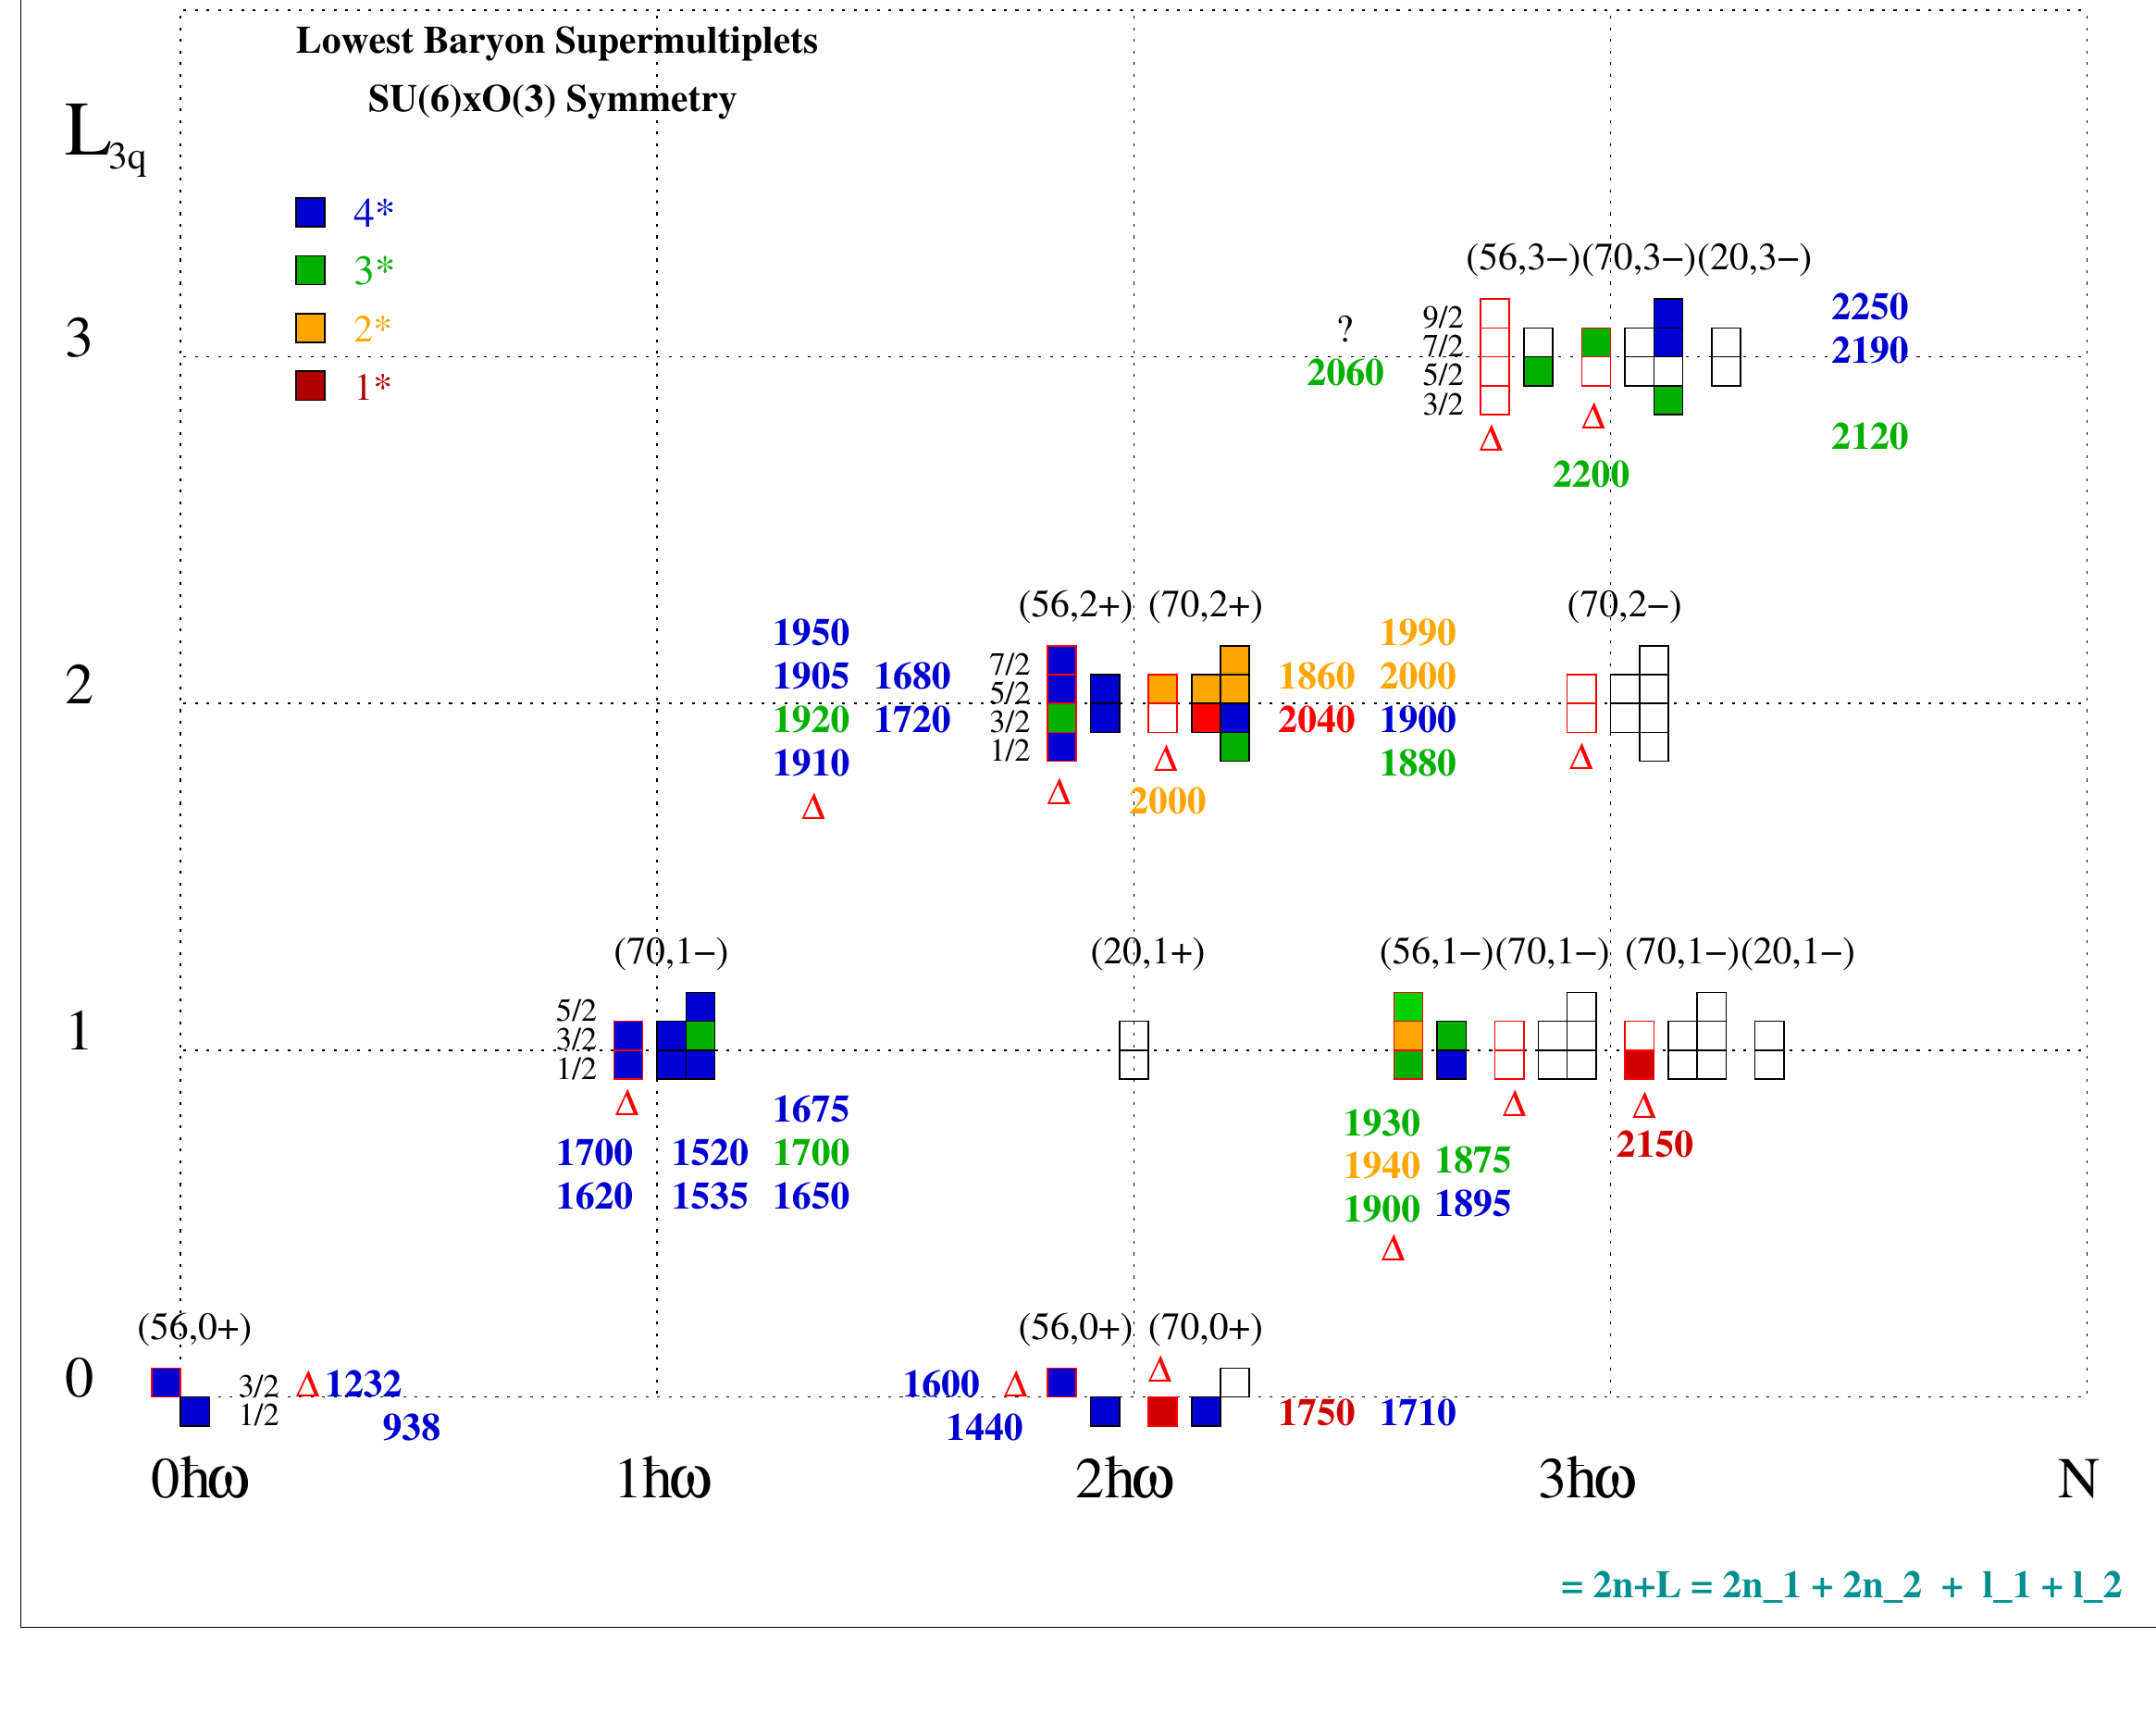
\includegraphics[width=0.9\textwidth]{Figures/baryon_supermultiplets.png}
  \caption{Distribution of the lowest baryon supermultiplets in the
  $\mathrm{SU}(6)\times O(3)$ harmonic-oscillator model as a function of orbital
  angular momentum $L$ and band number $N = 2n + L$, with the established
  $N^{*}$ and $\Delta^{*}$ assignments. Adapted from the lecture slides
  (week 20, "Multiplets $\leftrightarrow$ known $N^*$, $\Delta^*$-states").}
  \label{fig:baryon-supermultiplets}
\end{figure}

\FloatBarrier

% ============================================================
\subsection{Finding color in experiments}
\label{subsec:color-experiment}

Color was introduced to save the quark model, but its threefold character is not a
bookkeeping device: it can be measured. The cleanest counting experiment is the
annihilation of electron--positron pairs into hadrons through a virtual photon. Since the
photon couples to the quark electric charge, the total annihilation cross section into a
quark--antiquark pair of charge $e_f$ is, summing over all kinematically accessible final
states,
\begin{equation}
    \sigma_{\text{tot}}(e^+e^- \to f\bar f)
    \;\propto\; \sum_{\text{all } f\bar f \text{ pairs}} \frac{4\pi e_f^{2}}{3s},
\end{equation}
where $\sqrt{s}$ is the center-of-mass energy \cite[Ch.~10]{Amsler2018}. Normalizing the
hadronic cross section to that for muon pairs removes the common kinematic factors and
isolates the charge and color content,
\begin{equation}
    R = \frac{\sigma_{\text{tot}}(e^+e^- \to q\bar q)}
             {\sigma_{\text{tot}}(e^+e^- \to \mu^+\mu^-)}
      = N_{C} \sum_q e_q^{2},
    \label{eq:R-ratio}
\end{equation}
the factor $N_{C}$ arising because each quark flavor is produced in $N_{C}$ distinguishable
colors \cite[Ch.~10]{Amsler2018}.

The predictive power of \eqref{eq:R-ratio} lies in its step structure. As the energy
crosses the threshold for producing a new flavor, the ratio increases by $e_q^{2} N_{C}$.
Taking $N_{C} = 3$ one predicts $R = 2$ in the region where only the $u$, $d$ and $s$ quarks
are produced, rising to $R = 10/3$ above the charm threshold and to $R = 11/3$ once the
bottom quark contributes,
\begin{align}
    u,d:   &\quad \big(\tfrac{2}{3}\big)^2 + \big(\tfrac{1}{3}\big)^2 = \tfrac{5}{9}
            \;\Rightarrow\; \tfrac{5}{9}\,N_{C}, \nonumber\\
    u,d,s: &\quad \big(\tfrac{2}{3}\big)^2 + 2\big(\tfrac{1}{3}\big)^2 = \tfrac{2}{3}
            \;\Rightarrow\; \tfrac{2}{3}\,N_{C}\;(=2\ \text{for}\ N_{C}=3), \\
    u,d,s,c:   &\quad \;\Rightarrow\; \tfrac{10}{9}\,N_{C}, \nonumber\\
    u,d,s,c,b: &\quad \;\Rightarrow\; \tfrac{11}{9}\,N_{C}. \nonumber
\end{align}
The measured value of $R$ in the continuum between the resonances matches these
predictions only for $N_{C} = 3$, which is the central experimental statement that there are
three colors \cite[Ch.~10]{Amsler2018}. Figure~\ref{fig:R-ratio-steps} shows the
leading-order prediction with its characteristic increases at the open-flavor thresholds.

\begin{figure}[htbp]
    \centering
    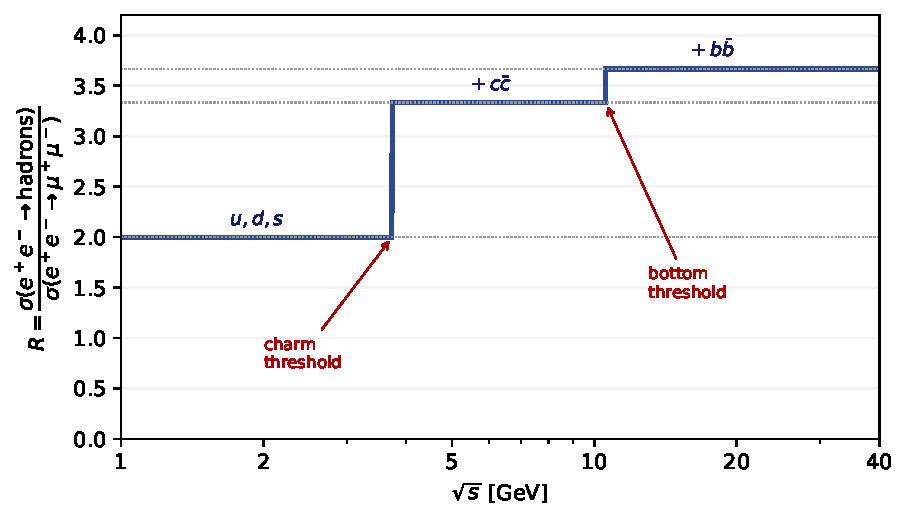
\includegraphics[width=0.7\textwidth]{Figures/R_ratio_steps.pdf}
    \caption{Leading-order prediction for the ratio $R = \sigma(e^+e^- \to
    \text{hadrons})/\sigma(e^+e^- \to \mu^+\mu^-) = N_{C} \sum_q e_q^2$ as a function of
    $\sqrt{s}$, for $N_{C} = 3$. The ratio increases by $e_q^2 N_{C}$ each time the energy
    crosses the threshold for producing a new quark flavor, giving $R = 2$ ($u,d,s$),
    $R = 10/3$ (adding $c$) and $R = 11/3$ (adding $b$). The smooth resonances are omitted.}
    \label{fig:R-ratio-steps}
\end{figure}

\begin{figure}[htbp]
  \centering
  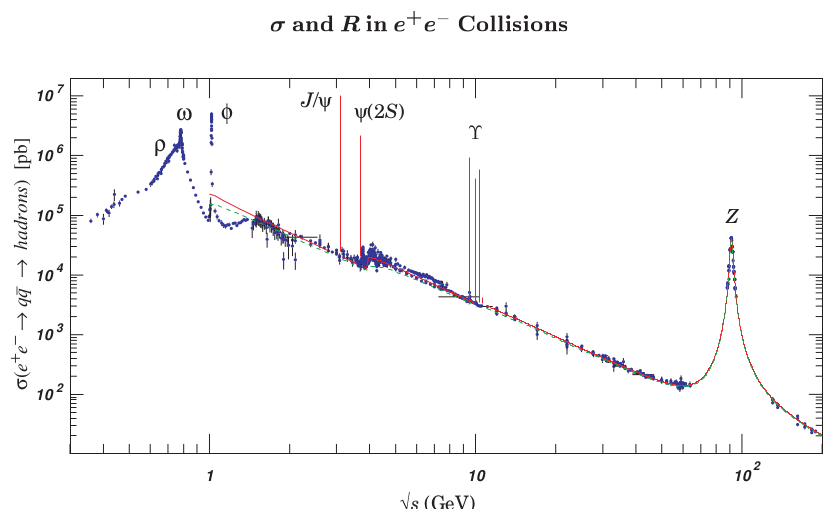
\includegraphics[width=0.9\textwidth]{Figures/R_measured_PDG.png}
  \caption{Measured cross section $\sigma(e^+e^-\to\mathrm{hadrons})$ (closely
  tracking the ratio $R$) over the full $\sqrt{s}$ range, showing the
  $\rho/\omega/\phi$ region, the narrow $J/\psi$ and $\psi(2S)$, the
  $\Upsilon$ states and the $Z$ pole. The smooth continuum between resonances
  sits on the plateaux predicted by $R = N_{C}\sum_q e_q^2$, requiring $N_{C}=3$.
  PDG compilation, adapted from the lecture slides (week 20, "Color -
  Experimental evidence for $N_C = 3$").}
  \label{fig:R-measured}
\end{figure}

The same factor of three appears in two further measurements. The decay $\pi^0 \to 2\gamma$
proceeds through a quark triangle whose amplitude is enhanced by the color sum, so that the
partial width scales as $N_{C}^{2}$ and the predicted rate agrees with experiment only for
three colors; without color the neutral-pion lifetime would be about nine times longer.
Likewise, the hadronic branching ratio of the $W^{+}$ boson, close to $66\%$, carries a
factor of three for each available quark color in the $u\bar d$ and $c\bar s$ channels
\cite[Ch.~10]{Amsler2018}. Taken together, the $e^+e^-$ ratio, the $\pi^0$ lifetime and the
$W$ branching fractions all point to the same conclusion, $N_{C} = 3$, which is the
experimental basis of QCD.

A related experimental fact, the strong suppression of flavor-changing neutral currents
such as $K^{+} \to \pi^{+}\nu\bar\nu$, is accounted for by the GIM mechanism and the
Cabibbo theory and was historically tied to the prediction of the charm quark, whose
$c\bar c$ bound states first appeared as the narrow $J/\psi$ resonance discussed in the
following section.

\FloatBarrier
\section{Hadron spectrometry}
\label{sec:hadron-spectrometry}

The colour degree of freedom introduced in Sect.~\ref{subsec:color-experiment} completes the
quark model of the light hadrons, but the most stringent test of the model came from a
different direction: the discovery of heavy quarks and the rich spectroscopy of the bound
states they form. A heavy quark and its antiquark bind into a non-relativistic,
hydrogen-like system whose level structure can be computed from a static potential, in
close analogy to positronium. The agreement between the measured and predicted spectra of
charmonium ($c\bar c$) and bottomonium ($b\bar b$) is one of the cleanest confirmations of
the quark picture and of the short- and long-distance behaviour of the strong force. This
section follows that development. It begins with the discovery of the $J/\psi$, develops the
description of unstable states as resonances, explains the anomalously small $J/\psi$ width
through the OZI rule, introduces the quark--antiquark potential and confinement, and then
works through the quarkonium spectra. It closes with the exotic states discovered since
2003, which do not fit the simple $q\bar q$ and $qqq$ scheme.

% ============================================================
\subsection{The \texorpdfstring{$J/\psi$}{J/psi} discovery}
\label{subsec:jpsi-discovery}

In November 1974 two groups announced, almost simultaneously, the observation of an
extraordinarily narrow resonance near $3.1\,\mathrm{GeV}$---an event so consequential for
particle physics that it became known as the ``November revolution''
\cite[Ch.~8]{Amsler2018}. At the Brookhaven National Laboratory, a group led by
J.~J.~Aubert studied the reaction $p + \mathrm{Be} \to e^+e^- + \text{anything}$ and
observed a heavy particle, which they named $J$, in the $e^+e^-$ invariant-mass spectrum.
The electrons and positrons were identified by their Cherenkov radiation and time of
flight, and their momenta were measured in two magnetic spectrometers. At the same time, a
group led by J.~E.~Augustin working at the SPEAR storage ring at Stanford studied
electron--positron annihilation, $e^+e^- \to \text{hadrons},\,\mu^+\mu^-,\,e^+e^-$, and
found a narrow resonance, which they named $\psi$. The particle is now universally
denoted $J/\psi$, with a measured mass $m(J/\psi) = 3096.9\,\mathrm{MeV}$
\cite[Ch.~8]{Amsler2018}.

Two features of the SPEAR observation fixed the interpretation. First, the production
mechanism---formation directly in $e^+e^-$ annihilation through a single virtual
photon---requires the state to carry the photon's quantum numbers, $J^{PC} = 1^{--}$, just
as the $\rho$ meson does. Second, the resonance was extraordinarily narrow: the apparent
width seen at SPEAR was limited entirely by the experimental energy resolution, implying a
true width well below the few-MeV scale typical of strongly decaying hadrons. A state with
mass $3.1\,\mathrm{GeV}$ and a width of at most a few MeV is anomalous, since the available
phase space for strong decay is enormous. The resolution of this puzzle was the
identification of the $J/\psi$ as the $1\,{}^3S_1$ bound state of a new, heavy
quark--antiquark pair, $c\bar c$, carrying the new quantum number \emph{charm}, with its
narrowness explained by the OZI rule (Sect.~\ref{subsec:ozi-width})
\cite[Ch.~8]{Amsler2018}.

% ------------------------------------------------------------
% FIGURE SUGGESTION:
% Two-panel discovery figure. (left) BNL e+e- invariant-mass spectrum from
% p+Be -> e+e- + X (Aubert et al.), showing the sharp J peak near 3.1 GeV on a
% smooth background; (right) the three SPEAR excitation curves (Augustin et al.)
% for e+e- -> hadrons, e+e- -> mu+mu-, e+e- -> e+e- versus E_cms, each showing the
% psi resonance. Reproduce from the week 21 VL1 "Summary: J/psi discovery (1974)"
% slide (BNL spectrum and SPEAR scans).
% \begin{figure}[t]
%   \centering
%   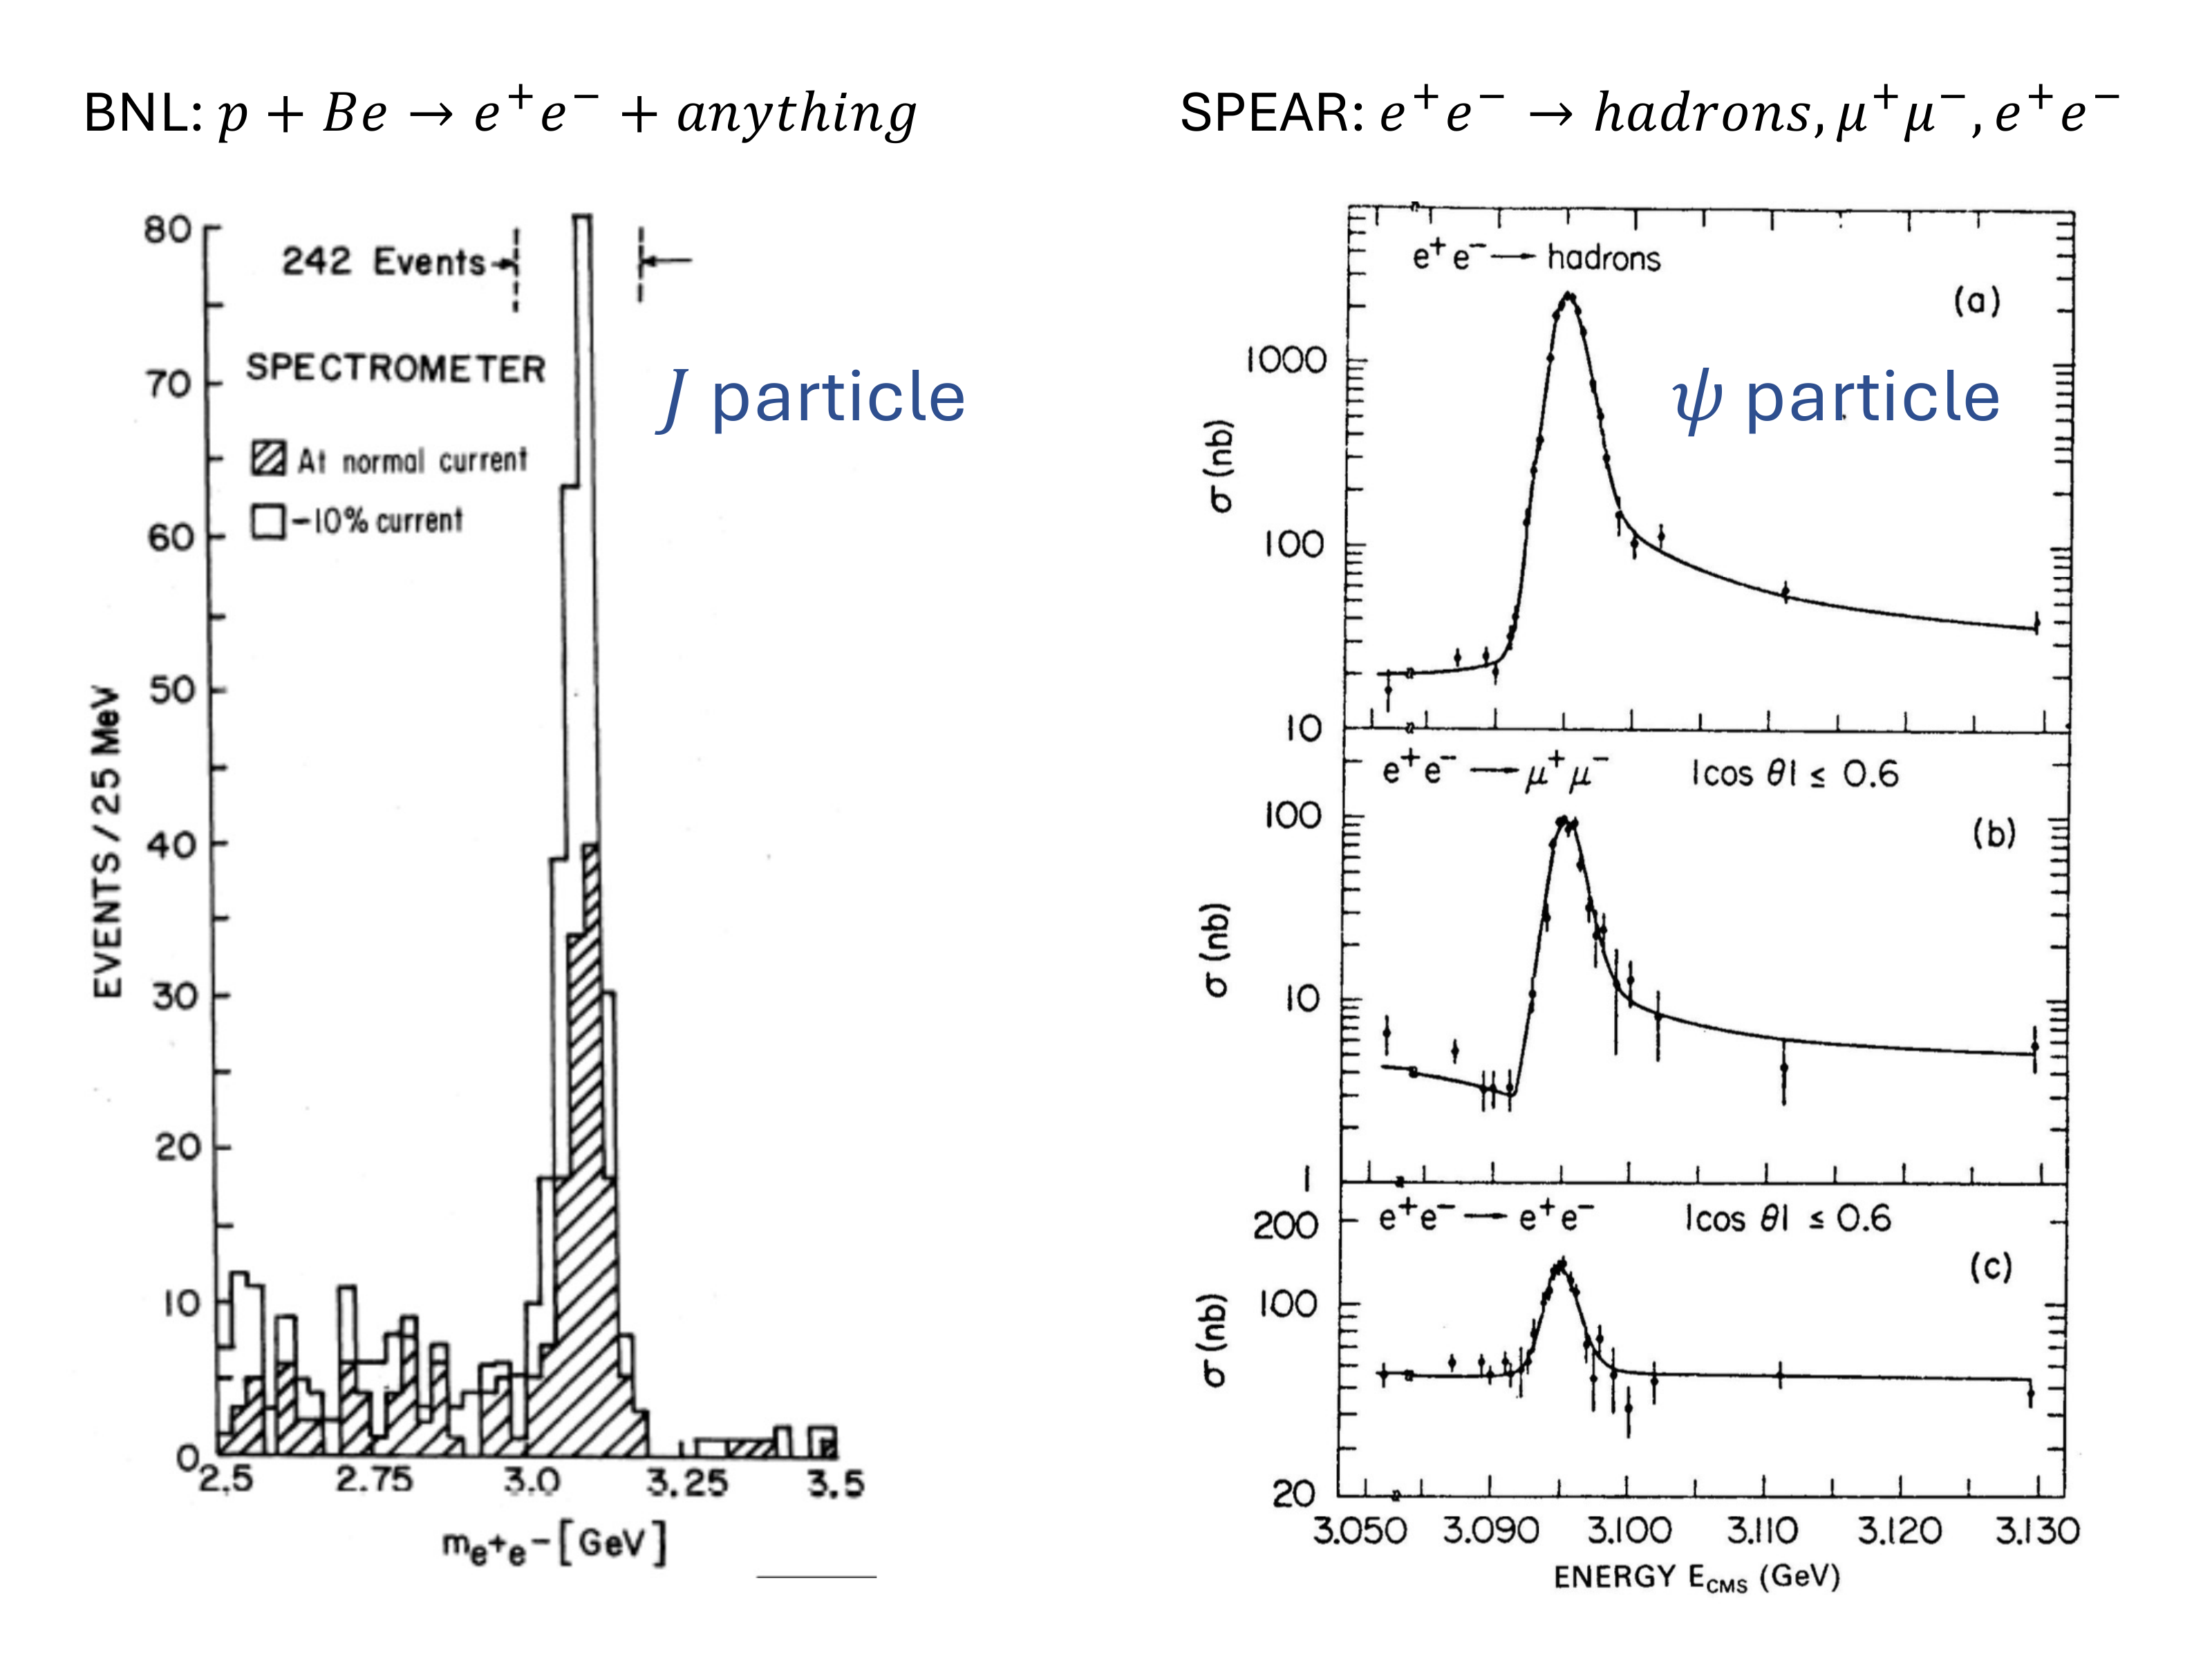
\includegraphics[width=0.95\textwidth]{Figures/jpsi_discovery.pdf}
%   \caption{The 1974 discovery of the $J/\psi$. Left: the heavy particle $J$ seen
%   by the BNL group in $p+\mathrm{Be}\to e^+e^-+X$. Right: the resonance $\psi$ seen
%   at SPEAR in three annihilation channels, fixing $J^{PC}=1^{--}$.}
%   \label{fig:jpsi-discovery}
% \end{figure}
% ------------------------------------------------------------

\FloatBarrier

% ============================================================
\subsection{Resonances}
\label{subsec:resonances}

An unstable particle is observed not as a sharp mass but as a peak of finite width in a
cross section or invariant-mass distribution. The shape of that peak follows directly from
the exponential character of radioactive decay. By Fermi's golden rule the transition rate
per unit time from an initial to a final state is
\begin{equation}
    T_{if} = 2\pi\,|\mathcal{M}|^2\,\rho(E_f),
    \label{eq:fermi-golden}
\end{equation}
where $\mathcal{M}$ is the transition matrix element and $\rho(E_f)$ the density of final
states. A sample of $N$ particles then obeys $\mathrm{d}N = -N\,T_{if}\,\mathrm{d}t$, whose
solution is the familiar exponential law $N = N_0\,e^{-t/\tau} = N_0\,e^{-\Gamma t}$, where
the mean lifetime $\tau$ and the total width $\Gamma$ are related by $\Gamma\tau = \hbar = 1$
in natural units.

A stable state of energy $E_0$ is described by a wavefunction $\psi(t) = \psi_0\,e^{-iE_0 t}$
whose probability density $|\psi(t)|^2 = |\psi_0|^2$ is constant in time. For an unstable
state the probability density must instead decay exponentially, which is achieved by giving
the energy a small imaginary part, so that
\begin{equation}
    \psi(t) = \psi(0)\,e^{-iE_0 t}\,e^{-t/2\tau},
    \qquad
    |\psi(t)|^2 = |\psi(0)|^2\,e^{-t/\tau}.
    \label{eq:decaying-state}
\end{equation}
The damped oscillation \eqref{eq:decaying-state} is no longer a single frequency: it
contains a spread of energies. The energy content is obtained from the Fourier transform,
\begin{equation}
    f(E) \sim \int_0^\infty \psi(0)\,e^{-i\left[(E_0 - E)t - i t/2\tau\right]}\,\mathrm{d}t
         \;=\; \frac{\psi(0)}{(E_0 - E) - i/(2\tau)} .
    \label{eq:fourier-resonance}
\end{equation}
The probability of finding the state with energy $E$ is then proportional to $|f(E)|^2$, and
with $\tau = 1/\Gamma$ this yields the \emph{non-relativistic Breit--Wigner distribution}
\begin{equation}
    |f(E)|^2 \;\propto\; \frac{(\Gamma/2)^2}{(E_0 - E)^2 + (\Gamma/2)^2},
    \label{eq:breit-wigner-intensity}
\end{equation}
a bell-shaped curve peaked at $E = E_0$ with a full width at half maximum equal to $\Gamma$
(Fig.~\ref{fig:breit-wigner}).

\begin{figure}[t]
    \centering
    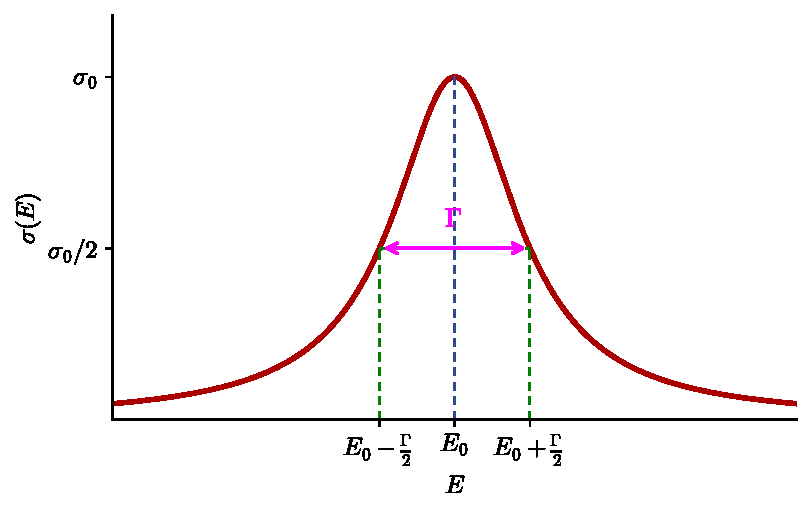
\includegraphics[width=0.62\textwidth]{Figures/breit_wigner.pdf}
    \caption{The non-relativistic Breit--Wigner line shape \eqref{eq:breit-wigner-intensity}.
    The peak sits at the resonance energy $E_0$ and the full width at half maximum equals the
    total width $\Gamma$.}
    \label{fig:breit-wigner}
\end{figure}

Resonances are most fundamentally described not by the intensity \eqref{eq:breit-wigner-intensity}
but by the underlying complex amplitude
\begin{equation}
    \mathrm{BW}(E) = \frac{\Gamma/2}{(E_0 - E) - i\,\Gamma/2}.
    \label{eq:breit-wigner-amplitude}
\end{equation}
Introducing the phase shift $\delta$ through $\cot\delta = 2(E_0 - E)/\Gamma$, the amplitude
takes the compact form
\begin{equation}
    f(E) = \frac{1}{\cot\delta - i} = e^{i\delta}\sin\delta,
    \label{eq:amplitude-phaseshift}
\end{equation}
which can equally be derived from the $S$-matrix. As the energy sweeps across the resonance,
the phase $\delta$ rises through $90^\circ$ at $E = E_0$, and the amplitude $f(E)$ traces a
circle in the complex plane---the \emph{Argand diagram}---reaching the top of the circle at
resonance. Real hadronic resonances are usually more complicated than this idealized
picture: overlapping resonances, several open decay channels, and energy-dependent widths
all distort the simple circle. The $\Delta(1232)$, seen as the $P_{33}$ partial wave in
$\pi N \to \pi N$ scattering, is the textbook example whose real and imaginary parts
approximate, but do not exactly reproduce, the ideal Breit--Wigner behaviour
\cite[Ch.~9]{Amsler2018}.

For a resonance formed in the collision of two particles with spins $s_1$ and $s_2$, the
energy dependence of the cross section combines the Breit--Wigner factor with the spin
multiplicities,
\begin{equation}
    \sigma(E) = \frac{4\pi}{k^2}\,
    \frac{\Gamma^2/4}{(E - E_R)^2 + \Gamma^2/4}\,
    \frac{2J + 1}{(2s_1 + 1)(2s_2 + 1)},
    \label{eq:resonance-cross-section}
\end{equation}
where $1/k = \lambda/2\pi = \hbar/p$ is the reduced de~Broglie wavelength of the colliding
particles in the centre-of-mass frame, $E$ the centre-of-mass energy, and $J$ the resonance
spin. Equation~\eqref{eq:resonance-cross-section} is the tool used in
Sect.~\ref{subsec:ozi-width} to extract the true $J/\psi$ width from the measured reaction
rate.

% ------------------------------------------------------------
% FIGURE SUGGESTION:
% Two-panel resonance figure complementing the generated Breit-Wigner plot.
% (left) Argand diagram: the amplitude T = BW(E) tracing the unitarity circle in
% the complex plane with the phase shift delta and the resonance point R at the top;
% (right) the measured P_33 (Delta(1232)) partial-wave amplitude in pi N -> pi N,
% real and imaginary parts versus W. Reproduce from the week 21 VL1 "Summary:
% Resonance" slide.
% \begin{figure}[t]
%   \centering
%   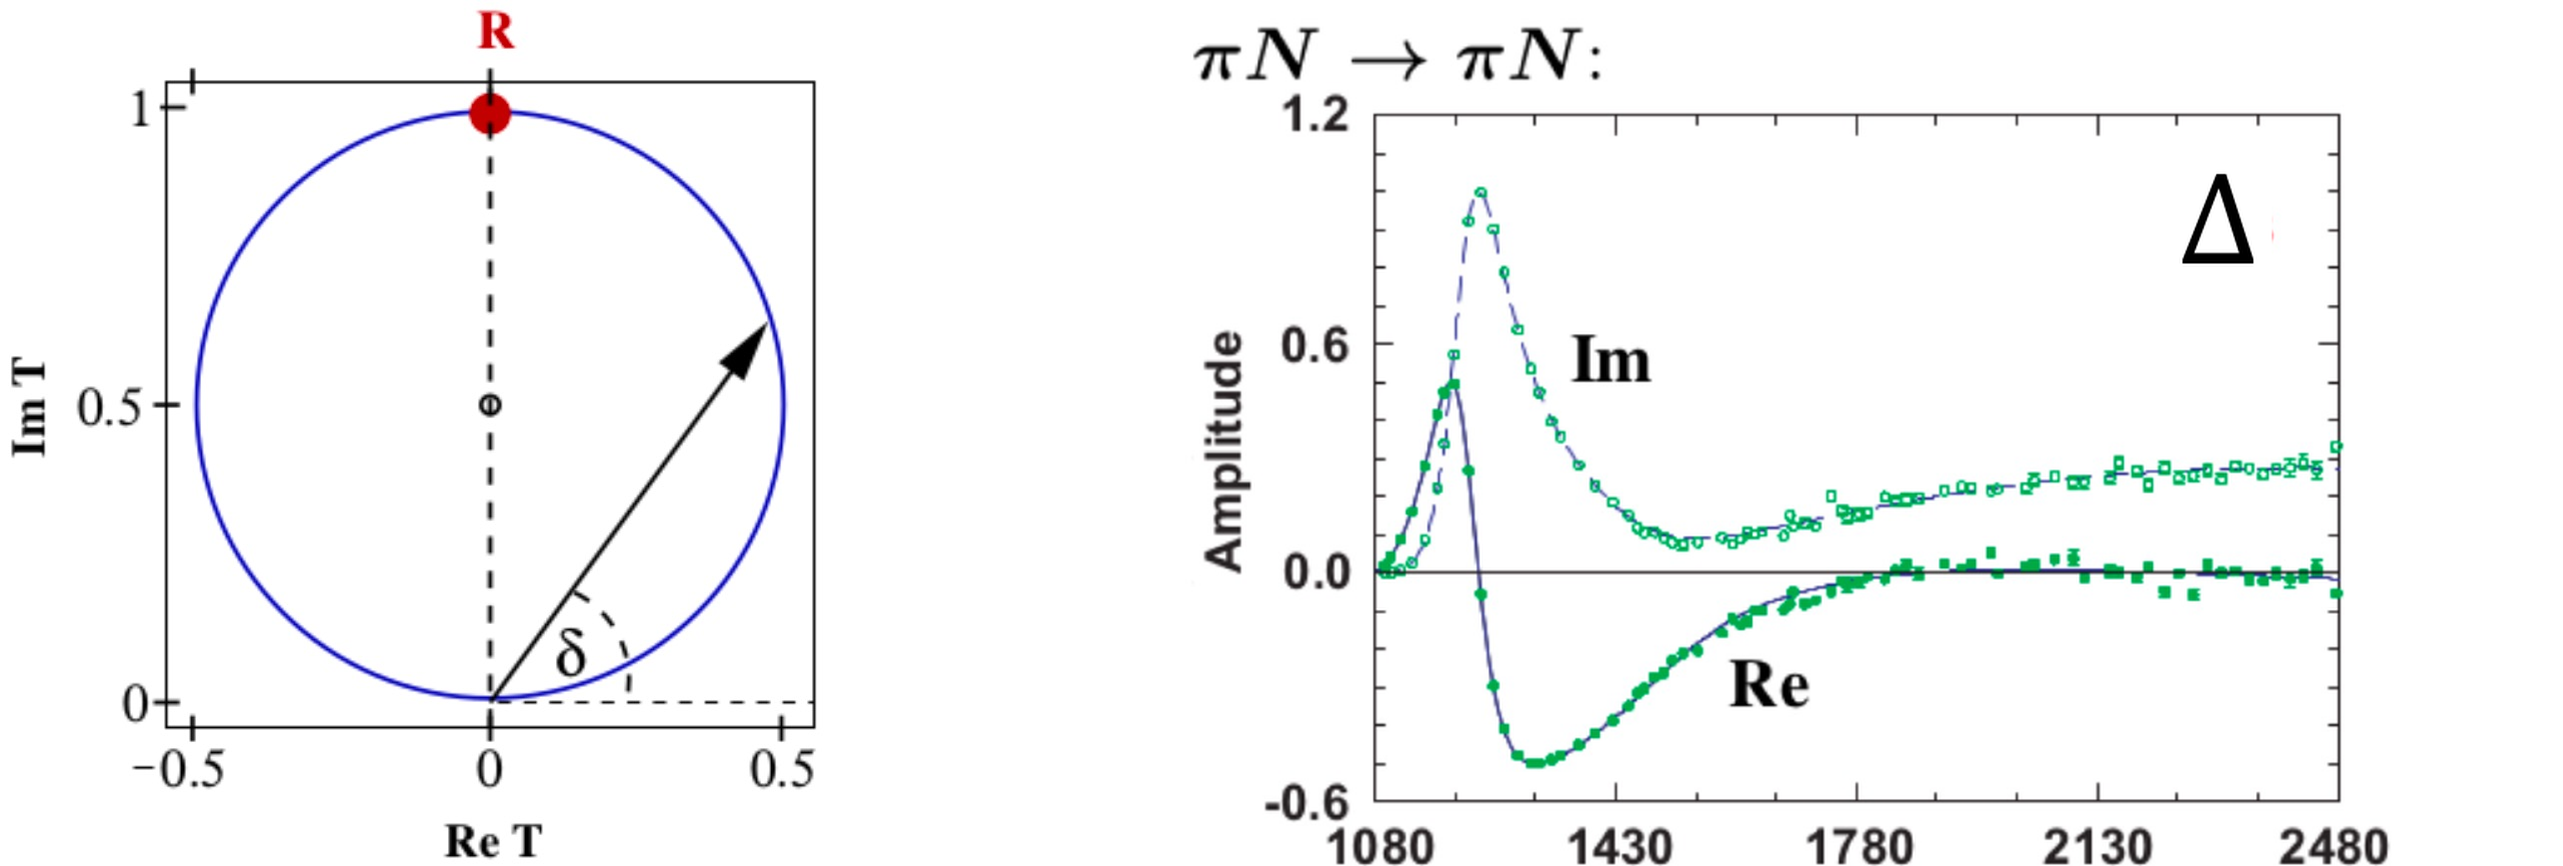
\includegraphics[width=0.9\textwidth]{Figures/argand_delta.pdf}
%   \caption{Left: Argand diagram of the resonant amplitude
%   \eqref{eq:amplitude-phaseshift}. Right: the $P_{33}$ ($\Delta(1232)$)
%   partial-wave amplitude in $\pi N$ scattering, illustrating departures from the
%   ideal circle.}
%   \label{fig:argand-delta}
% \end{figure}
% ------------------------------------------------------------

\FloatBarrier

% ============================================================
\subsection{The OZI rule and the width of the \texorpdfstring{$J/\psi$}{J/psi}}
\label{subsec:ozi-width}

The narrowness of the $J/\psi$ is explained by its position below the threshold for decay
into a pair of charmed mesons. The lightest charmed mesons have masses $m(D^\pm) =
1869\,\mathrm{MeV}$ and $m(D^0) = 1865\,\mathrm{MeV}$, so that the lowest open-charm
threshold lies near $2m(D) \approx 3.74\,\mathrm{GeV}$, well above the $J/\psi$ mass of
$3096.9\,\mathrm{MeV}$ \cite[Ch.~8]{Amsler2018}. The $J/\psi$ therefore cannot dissociate
into a $D\bar D$ pair, in which the initial $c$ and $\bar c$ are simply carried off into the
final mesons along connected quark lines. It is forced instead to decay through the
annihilation of the $c\bar c$ pair into light hadrons, a process governed by the
Okubo--Zweig--Iizuka (OZI) rule: decay amplitudes whose quark-line diagrams can be cut into
two disconnected pieces by severing only gluon lines are strongly suppressed.

The suppression can be quantified by counting gluons. In the decay $J/\psi \to 3\pi$ the
$c\bar c$ must annihilate completely, and no colour can be transmitted from the colour-singlet
$c\bar c$ state to the colour-singlet final hadrons except through a colourless combination
of at least two gluons. The quantum numbers tighten this further: an $n$-gluon system carries
charge conjugation $C = (-1)^n$, and matching the $J^{PC} = 1^{--}$ of the $J/\psi$ together
with colour neutrality requires at least three gluons, $n \geq 3$. Each of these gluons is
hard, since it must carry a momentum of order the charm mass, $q^2 \sim m_\psi^2$, where the
strong coupling is small. The annihilation rate is therefore proportional to $\alpha_s^6$
and is strongly suppressed, which accounts for the long lifetime and small width
\cite[Ch.~8]{Amsler2018}. By contrast, a heavier vector charmonium state lying above the
open-charm threshold, such as the $\psi(3770)$, can decay into $D\bar D$ through connected
quark lines requiring only a single soft gluon to create the additional light quark pair;
such states are correspondingly broad.

Because the apparent width of the $J/\psi$ is dominated by the experimental resolution, the
true width is far smaller than the observed peak and cannot be read off directly. It is
instead reconstructed from the total reaction rate and the leptonic branching ratio, using
the resonance cross section \eqref{eq:resonance-cross-section}. The integral of the
measured peak, combined with the fraction of decays into a known channel such as
$e^+e^-$ or $\mu^+\mu^-$, fixes the partial widths and hence the total width, yielding a
value of order $0.1\,\mathrm{MeV}$---two orders of magnitude smaller than the width of a
typical light-quark resonance such as the $\rho$ ($\Gamma \approx 150\,\mathrm{MeV}$ at
$m \approx 770\,\mathrm{MeV}$).

\FloatBarrier

% ============================================================
\subsection{The quark--antiquark potential and confinement}
\label{subsec:qq-potential}

The success of treating quarkonium as a non-relativistic bound state rests on a static
potential between the heavy quark and antiquark. The standard parametrization, the
\emph{Cornell potential}, combines a short-distance Coulomb-like term with a long-distance
linear term,
\begin{equation}
    V_{Q\bar Q}(r) = -\frac{4}{3}\,\frac{\alpha_s}{r} + k\,r,
    \label{eq:cornell-potential}
\end{equation}
with a representative strong coupling $\alpha_s = 0.3$ and string tension
$k = 1\,\mathrm{GeV\,fm^{-1}}$ \cite[Ch.~9]{Amsler2018}. The colour factor $4/3$ arises from
the $\mathrm{SU}(3)_c$ structure of one-gluon exchange between a colour and an anticolour
charge. At small separations the Coulomb term dominates and the potential resembles that of
electromagnetism, reflecting the asymptotic freedom of QCD; at large separations the linear
term dominates and grows without bound, the hallmark of confinement
(Fig.~\ref{fig:cornell-potential}).

\begin{figure}[t]
    \centering
    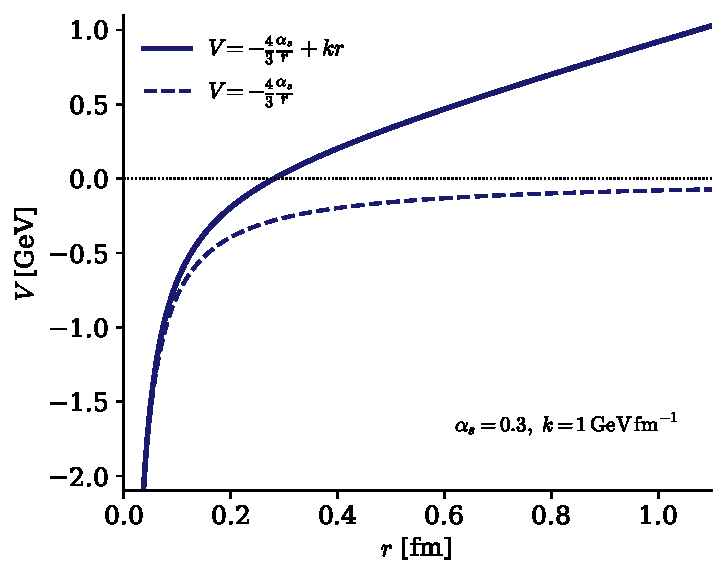
\includegraphics[width=0.6\textwidth]{Figures/cornell_potential.pdf}
    \caption{The Cornell quark--antiquark potential \eqref{eq:cornell-potential} for
    $\alpha_s = 0.3$ and $k = 1\,\mathrm{GeV\,fm^{-1}}$ (solid). The dashed curve shows the
    Coulomb-like term alone; the linear term produces the rising confining behaviour at
    large $r$.}
    \label{fig:cornell-potential}
\end{figure}

Spin-dependent corrections, suppressed by powers of the heavy-quark mass $m_Q$, generate the
fine and hyperfine structure of the spectrum. The spin--spin (contact) interaction,
\begin{equation}
    V_{SS} = \frac{8\pi\alpha_s}{9\,m_Q^2}\,\delta^3(\vec r)\,
    \vec S_Q \cdot \vec S_{\bar Q},
\end{equation}
splits states differing in total spin and acts only where the wavefunction overlaps at the
origin. The spin--orbit and tensor interactions,
\begin{align}
    V_{LS} &= \frac{1}{m_Q^2}\left(\frac{2\alpha_s}{r^3} - \frac{k}{2r}\right)
              \vec L \cdot \vec S, \\
    V_{T}  &= \frac{1}{m_Q^2}\,\frac{\alpha_s}{3r^3}
              \left(\frac{3\,(\vec S_Q\cdot\hat r)(\vec S_{\bar Q}\cdot\hat r)}{r^2}
              - \vec S_Q\cdot\vec S_{\bar Q}\right),
\end{align}
split the orbital multiplets and couple states of equal $J$ but different $L$ and $S$
\cite[Ch.~9]{Amsler2018}.

The linear term in \eqref{eq:cornell-potential} has a direct physical picture. Whereas the
electric field lines between two opposite charges spread out through space, giving the
familiar $1/r^2$ force, the colour field between a quark and an antiquark is squeezed into a
narrow flux tube, or string, of roughly constant energy per unit length. The force between
them is therefore approximately constant at large separation rather than falling off, so the
energy stored in the string rises linearly with distance. When enough energy is stored, it
becomes energetically favourable to create a new $q\bar q$ pair from the vacuum, the string
breaks, and two colour-singlet hadrons fly apart. This is why isolated colour charges are
never observed: pulling a quark out of a hadron produces more hadrons, not a free quark
\cite[Ch.~10]{Amsler2018}.

\FloatBarrier

% ============================================================
\subsection{Regge trajectories}
\label{subsec:regge}

Independent evidence for the linear confining potential comes from the systematics of the
light mesons. If the mass of a highly excited light meson resides almost entirely in the
energy of the gluonic string---the light quark masses being negligible---then a simple
rotating-string model predicts that the squared mass grows linearly with the total angular
momentum. The data bear this out strikingly: plotting $M^2$ against $J$ for the leading
$\rho/a$ and $\omega/f$ families produces straight lines, the \emph{Regge trajectories}
(Fig.~\ref{fig:regge}), with the $\rho(770)$, $f_2(1270)/a_2(1318)$,
$\omega_3(1670)/\rho_3(1700)$, $a_4(2020)/f_4(2050)$, $\rho_5(2350)$ and
$a_6(2450)/f_6(2510)$ falling on a common slope of order $1\,\mathrm{GeV^2}$ per unit of
spin \cite[Ch.~9]{Amsler2018}. The linearity of these trajectories is exactly what the
linear term of \eqref{eq:cornell-potential} implies for the large-$r$ behaviour of the
quark--antiquark system, tying the light-meson spectroscopy to the same confining dynamics
that governs the heavy quarkonia.

\begin{figure}[t]
    \centering
    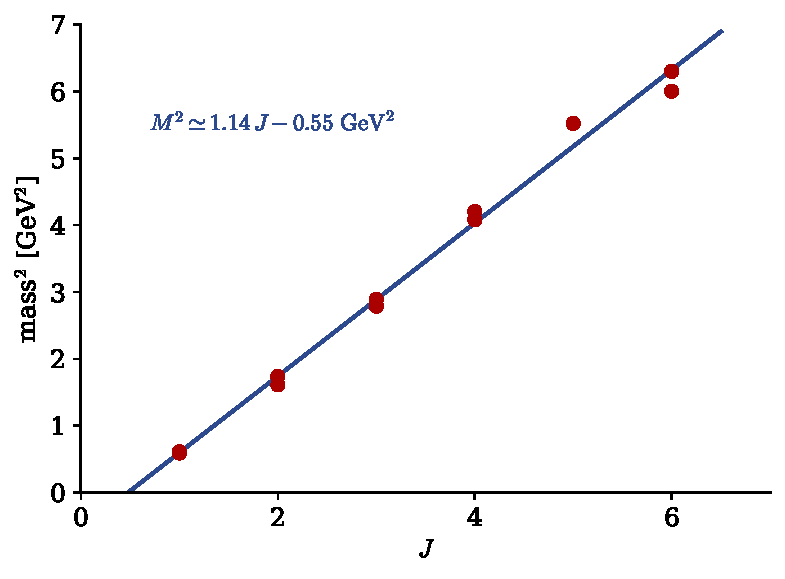
\includegraphics[width=0.62\textwidth]{Figures/regge_trajectory.pdf}
    \caption{Regge trajectory of the leading light mesons: the squared mass plotted against
    the total angular momentum $J$ falls on a straight line, consistent with a linear
    confining potential. The fitted slope is of order $1\,\mathrm{GeV^2}$ per unit spin.}
    \label{fig:regge}
\end{figure}

\FloatBarrier

% ============================================================
\subsection{The charmonium spectrum and potential models}
\label{subsec:charmonium-spectrum}

Because the charm quark is heavy, the $c\bar c$ system is non-relativistic and its spectrum
follows from solving the Schr\"odinger equation with the potential of
Sect.~\ref{subsec:qq-potential}. The states are labelled spectroscopically as
$n^{2S+1}L_J$, where $S$ is the total quark spin, $L$ the orbital angular momentum and $J$
the total angular momentum. A subtlety of nomenclature must be noted: for positronium the
principal quantum number is defined as $n = N + L + 1$, whereas for quarkonium the
convention $n = N + 1$ is used, where $N$ counts the radial nodes of the wavefunction
\cite[Ch.~9]{Amsler2018}.

The analogy with positronium is close in structure but vastly different in scale. Positronium
is bound by the electromagnetic interaction with coupling $\alpha = 1/137$ between particles
of mass $m_e = 0.511\,\mathrm{MeV}$, while charmonium is bound by the strong interaction with
$\alpha_s = 0.2$--$1$ between quarks of mass $m_c \approx 1600\,\mathrm{MeV}$. The
characteristic energy scale, which goes as $m\,\alpha^2$, is therefore larger for charmonium
by a factor of order $(m_c/m_e)(\alpha_s^2/\alpha^2) \sim 10^8$, so that positronium binding
energies measured in electron-volts correspond to charmonium splittings of hundreds of MeV.
The level ordering reflects the potential directly: because the Laplacian of the Cornell
potential is positive, $\nabla^2 V > 0$, the $P$ levels lie above the corresponding lower
$S$ levels, and indeed the $\chi_{cJ}(1P)$ states are found below the $\psi(2S)$
\cite[Ch.~9]{Amsler2018}. Potential models reproduce the measured charmonium spectrum well,
especially for the low-lying states.

% ------------------------------------------------------------
% FIGURE SUGGESTION:
% Side-by-side level schemes of charmonium and positronium drawn on a common
% spectroscopic grid (n^{2S+1}L_J), with the charmonium mass axis in GeV and the
% positronium binding-energy axis in eV, and the DD-bar threshold indicated on the
% charmonium side. Reproduce from the week 21 VL1 "Resulting spectrum" slide
% (charmonium vs positronium). A TikZ level diagram would be appropriate here.
% \begin{figure}[t]
%   \centering
%   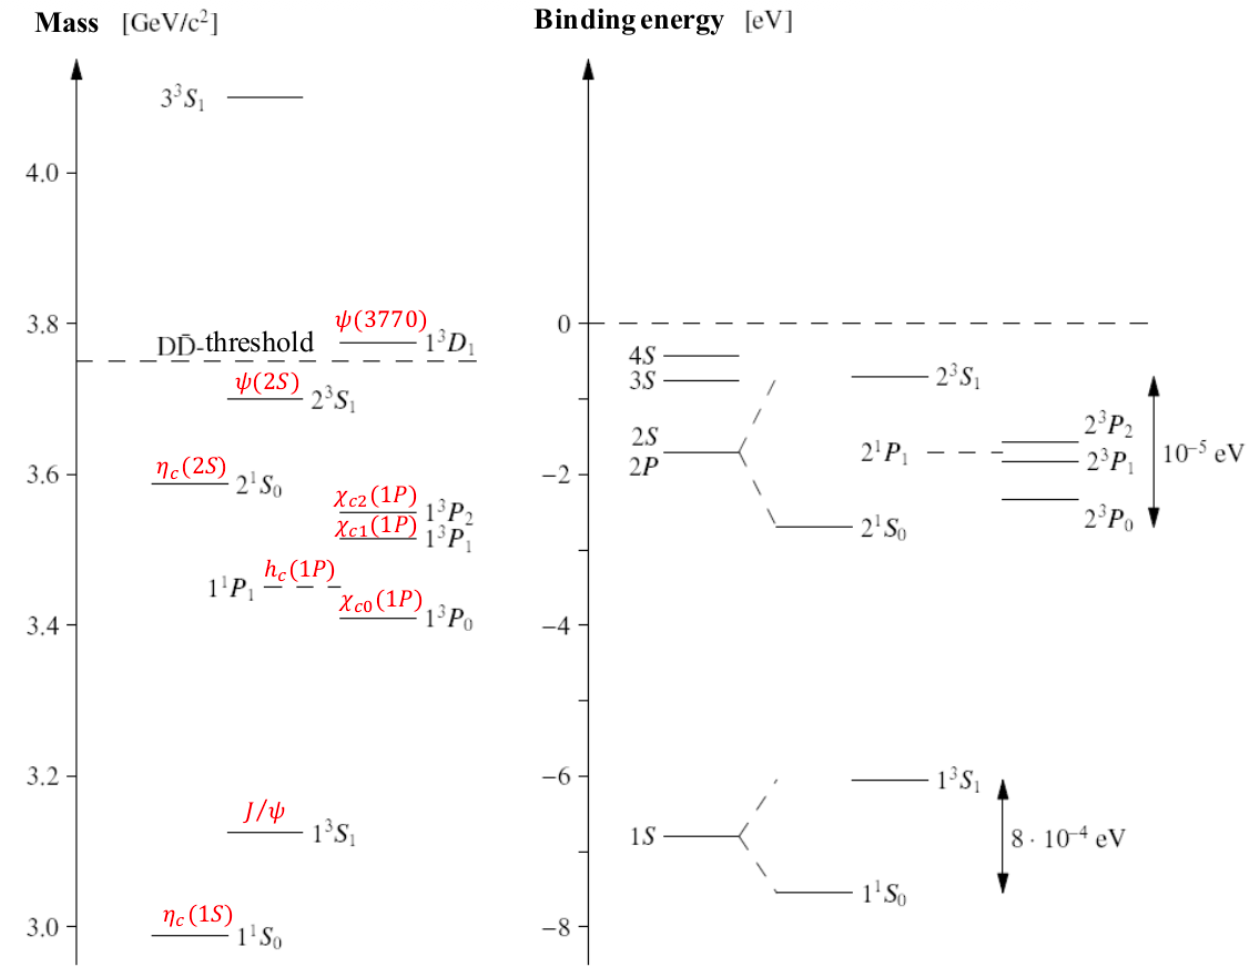
\includegraphics[width=0.85\textwidth]{Figures/charmonium_positronium.pdf}
%   \caption{The charmonium level scheme (left) compared with positronium (right),
%   showing the close structural analogy between an electromagnetically bound
%   $e^+e^-$ system and a strongly bound $c\bar c$ system.}
%   \label{fig:charmonium-positronium}
% \end{figure}
% ------------------------------------------------------------

\FloatBarrier

% ============================================================
\subsection{Probing charmonium: radiative decays and beam scans}
\label{subsec:charmonium-probes}

Only the $J^{PC} = 1^{--}$ states couple directly to the virtual photon and can therefore be
formed directly in $e^+e^-$ annihilation. The remaining charmonium levels are reached
indirectly, most cleanly through radiative transitions. The Crystal Ball experiment at SPEAR
mapped the spectrum by studying $e^+e^- \to \psi(2S) \to \gamma X$, in which the $\psi(2S)$
emits a photon and cascades to lower states \cite[Ch.~9]{Amsler2018}. The transitions obey
multipole selection rules. Electric dipole ($E1$) transitions have $\Delta L = 1$ and
$\Delta S = 0$ and connect the $1^{--}$ states to the $\chi_{cJ}$ ($J = 0, 1, 2$) states of
positive parity, so that the parity changes; magnetic dipole ($M1$) transitions have
$\Delta L = 0$ and $\Delta S = 1$ and connect to the $\eta_c$ states of $J = 0$ and negative
parity, leaving the parity unchanged. The measured masses of the principal states are
$\psi(1S) = 3096.9\,\mathrm{MeV}$, $\eta_c(1S) = 2983.9\,\mathrm{MeV}$,
$\psi(2S) = 3686.1\,\mathrm{MeV}$ and $\eta_c(2S) = 3637.7\,\mathrm{MeV}$. One early
radiative candidate, an $\eta_c'$ reported by Crystal Ball at $3592 \pm 5\,\mathrm{MeV}$,
was never confirmed and lay about $50\,\mathrm{MeV}$ too low for the potential models
\cite[Ch.~9]{Amsler2018}.

A limitation of the radiative method is that the spin-singlet $P$ state, the $h_c({}^1P_1)$,
cannot be reached from the $1^{--}$ levels by an allowed radiative transition. This state,
and precise widths in general, are accessible in proton--antiproton annihilation, exploited
by the E760 and E835 experiments at Fermilab. The advantage of the $p\bar p$ formation
technique is twofold. First, the antiproton beam energy can be tuned extremely precisely, so
that the resolution is set by the beam-momentum spread rather than by the calorimeter; E760
achieved a resolution of about $240\,\mathrm{keV}$, against the roughly $10\,\mathrm{MeV}$
typical of invariant-mass reconstruction in a detector. Second, this precision allows the
natural widths of the states to be resolved directly from a resonance scan. Scanning across
the $\chi_{c1}$ and $\chi_{c2}$ regions yielded
$\chi_{c1}(1P) = 3510.67 \pm 0.05\,\mathrm{MeV}$ and
$\chi_{c2}(1P) = 3556.17 \pm 0.07\,\mathrm{MeV}$, while the $\chi_{c0}$ was measured at a
mass of $3415.4\,\mathrm{MeV}$ with a width $\Gamma \approx 9.8\,\mathrm{MeV}$, and the
elusive $h_c(1P)$ was finally observed \cite[Ch.~9]{Amsler2018}. The same charmonium states
can also be produced in photoproduction, as pursued by the GlueX experiment through
$\gamma p \to \chi_{cJ}\,p$, which in addition offers a probe of the gluonic content of the
proton.

% ------------------------------------------------------------
% FIGURE SUGGESTION:
% Two related figures could be used here.
% (a) The Crystal Ball inclusive photon spectrum from e+e- -> psi(2S) -> gamma X,
%     with the radiative lines labelled, plus a level diagram with E1 (solid),
%     M1 (dashed), hadronic and 2-body EM transitions colour-coded.
% (b) The E760/E835 resonance scans across the chi_c1 and chi_c2 regions, cross
%     section versus sqrt(s), with the fitted Breit-Wigner curves.
% Reproduce from the week 21 VL1 "Charmonium Spectrum in Radiative Decays" and
% "Charmonium Spectrum in Beam Scans" slides.
% \begin{figure}[t]
%   \centering
%   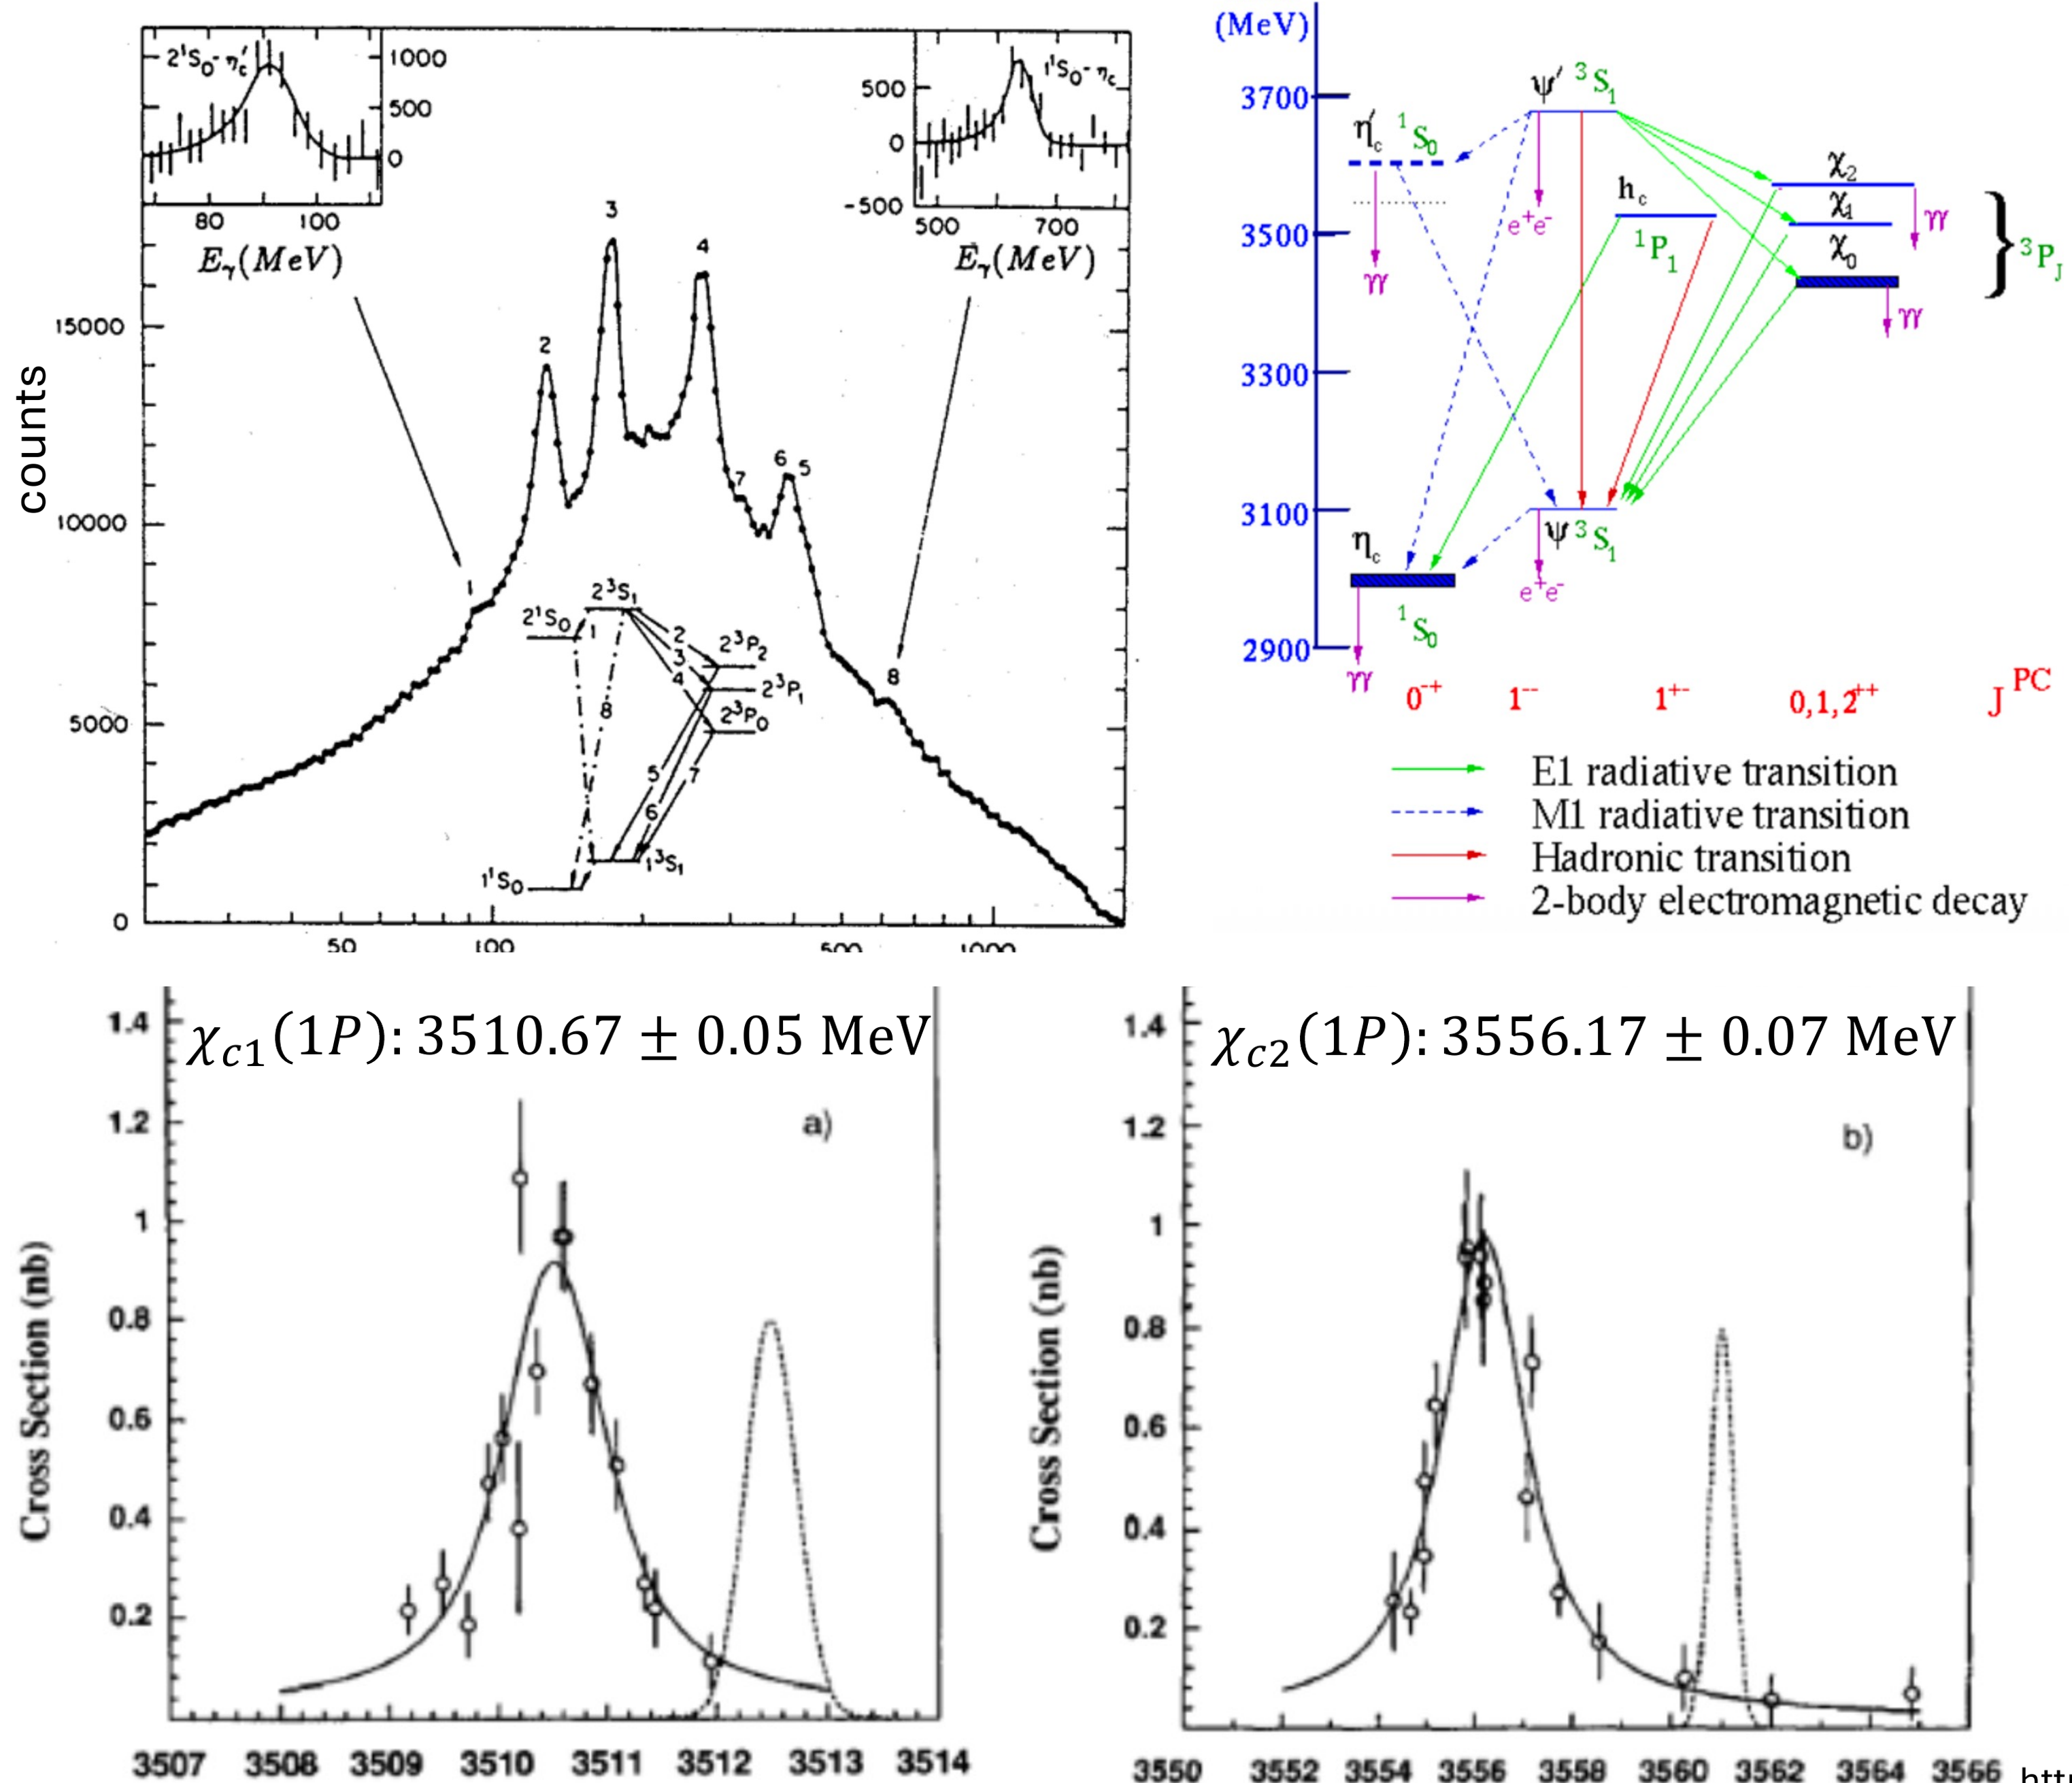
\includegraphics[width=0.9\textwidth]{Figures/charmonium_radiative_scan.pdf}
%   \caption{Probing the charmonium spectrum. Left: radiative photon spectrum from
%   $\psi(2S)\to\gamma X$ (Crystal Ball). Right: $p\bar p$ formation scans of the
%   $\chi_{c1}(1P)$ and $\chi_{c2}(1P)$ (E760/E835), whose narrow widths are
%   resolved by the precise beam momentum.}
%   \label{fig:charmonium-radiative-scan}
% \end{figure}
% ------------------------------------------------------------

\FloatBarrier

% ============================================================
\subsection{Bottomonium and the comparison of quarkonia}
\label{subsec:bottomonium}

Replacing the charm quark by the still heavier bottom quark produces bottomonium, the
$b\bar b$ system, observed in $e^+e^-$ annihilation at centre-of-mass energies near
$10\,\mathrm{GeV}$. Just as for charmonium, the lowest vector states---the $\Upsilon(1S)$,
$\Upsilon(2S)$ and $\Upsilon(3S)$---appear as very narrow resonances, for the same reason:
they lie below the threshold for decay into a pair of bottom mesons, which opens at
$10.558\,\mathrm{GeV}$. States above this threshold, such as the $\Upsilon(4S)$, decay
readily into $B\bar B$ and are broad. The resulting $b\bar b$ spectrum is closely analogous
to that of $c\bar c$ \cite[Ch.~9]{Amsler2018}.

A comparison of positronium, charmonium and bottomonium on a common spectroscopic footing
reveals both the universality and the limits of the potential picture. The lower-lying
levels have a very similar structure across all three systems, confirming that the same
functional form of the potential governs them. For the higher-lying levels, however, the
spacing decreases less rapidly than the $1/n^2$ law of a pure Coulomb potential, a direct
consequence of the linear confining term, and the $P$ states are positioned differently
relative to the $2S$ states in each system. The spin-singlet $h_b$ states, like their
charmonium counterpart, are not reached by radiative transitions and were instead first
observed by the Belle collaboration in $e^+e^- \to \Upsilon(5S) \to \pi^+\pi^- +
\text{hadrons}$, yielding the first observation of the $h_b(1P)$ and $h_b(2P)$
\cite[Ch.~9]{Amsler2018}. The $\psi$ and $\Upsilon$ families are now routinely used as
production engines for hadron spectroscopy at $e^+e^-$ colliders, with many discoveries
driven by data taken directly on resonance.

% ------------------------------------------------------------
% FIGURE SUGGESTION:
% Two figures are appropriate.
% (a) The R-ratio / e+e- cross section in the bottomonium region (sqrt(s) ~ 9.4-11.2
%     GeV) showing the narrow Upsilon(1S,2S,3S) peaks below, and the broad
%     Upsilon(4S) at, the B-meson threshold.
% (b) A three-panel comparison of the positronium, charmonium and bottomonium level
%     schemes on a shared n^{2S+1}L_J grid, illustrating the similar low-lying
%     structure and the differing high-lying spacings.
% Reproduce from the week 21 VL1 "R-plot revisited - Bottomonium" and "Comparison of
% e+e- vs cc vs bb" slides.
% \begin{figure}[t]
%   \centering
%   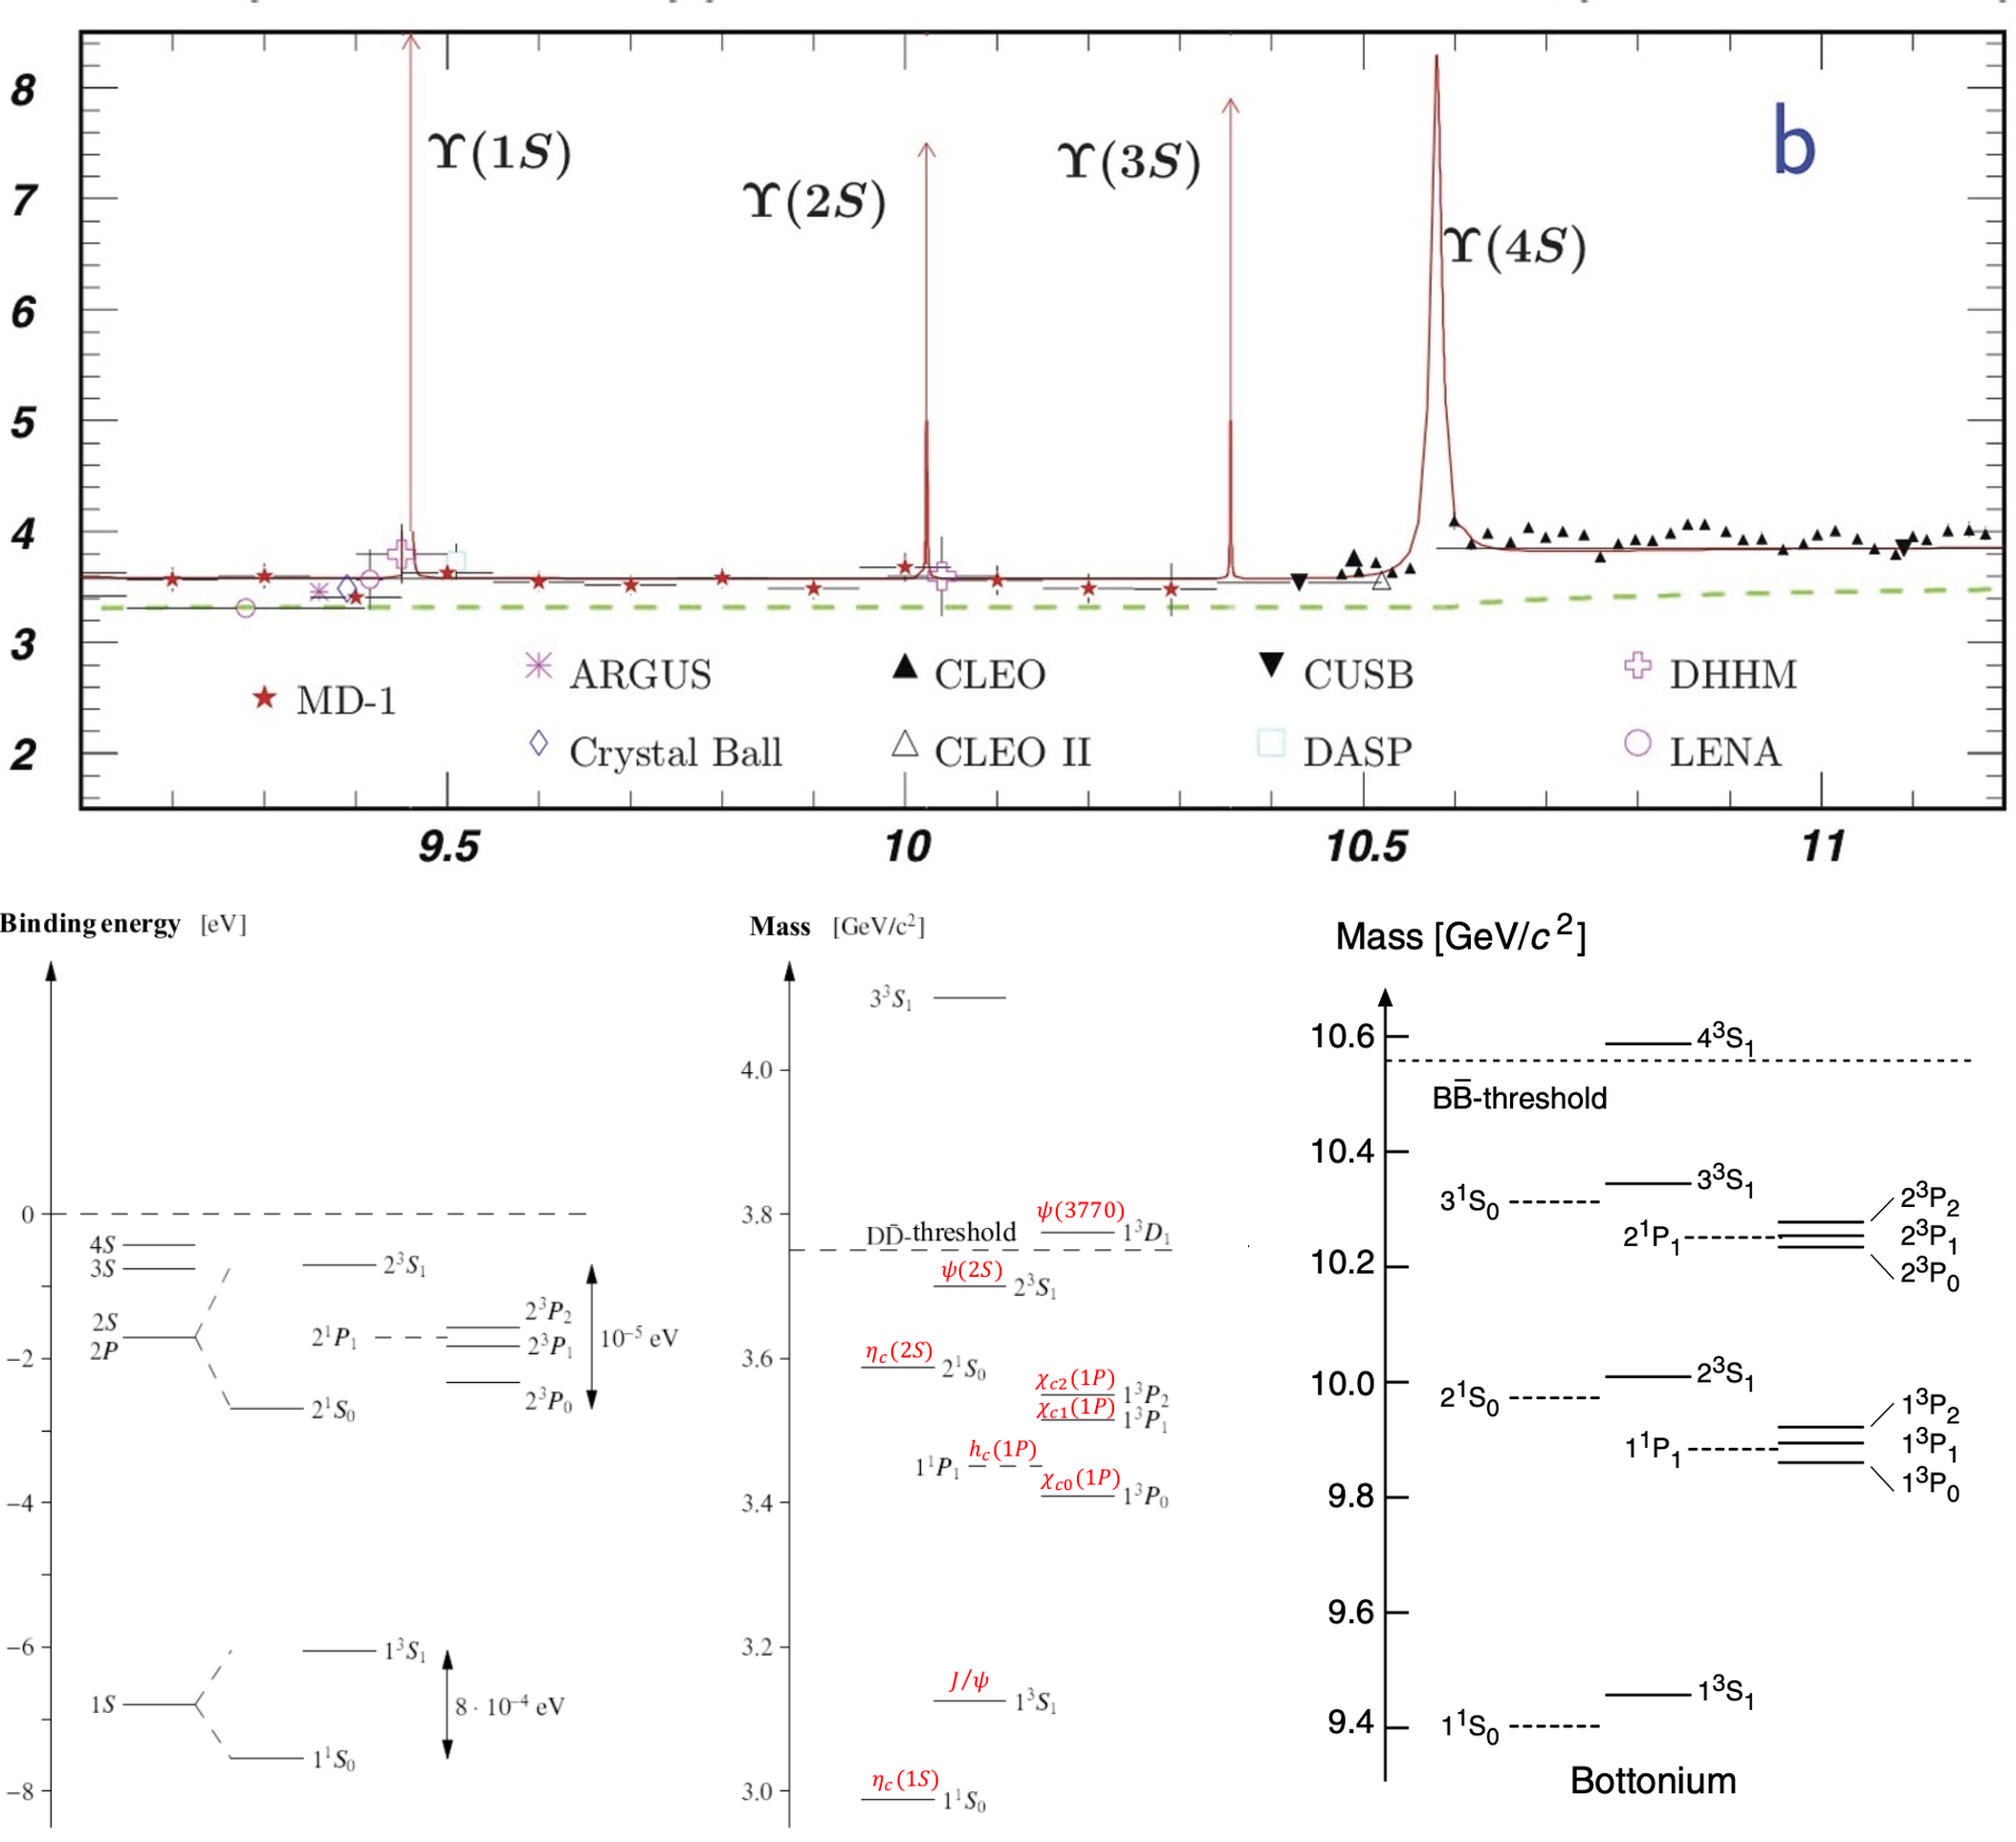
\includegraphics[width=0.95\textwidth]{Figures/bottomonium_comparison.pdf}
%   \caption{Left: the $b\bar b$ resonances in $e^+e^-$ annihilation, narrow below
%   the $B\bar B$ threshold at $10.558\,\mathrm{GeV}$ and broad above it. Right:
%   positronium, charmonium and bottomonium level schemes compared on a common grid.}
%   \label{fig:bottomonium-comparison}
% \end{figure}
% ------------------------------------------------------------

\FloatBarrier

% ============================================================
\subsection{Exotic States}
\label{subsec:exotic-states}

For the low-lying states the charmonium spectrum is a triumph of the potential model, but at
higher energies, near and above the open-charm threshold, the picture becomes far more
intricate. Since 2003 more than forty new states have been discovered that are difficult or
impossible to accommodate within the simple $q\bar q$ scheme, and several are manifestly
four-quark objects. Collectively known as the $XYZ$ states, they have driven a revival of
hadron spectroscopy, and the interpretation of most of them remains ambiguous
\cite[Ch.~16]{Amsler2018}.

The prototype is the $X(3872)$, discovered by the Belle collaboration in 2003 in the decay
$B^+ \to K^+ X$ with $X \to J/\psi\,\pi^+\pi^-$, and since confirmed by many experiments in
many modes. Its mass, $m(X) = 3871.64 \pm 0.06\,\mathrm{MeV}$, lies extraordinarily close to
the $D^0\bar D^{*0}$ threshold of $3871.68 \pm 0.07\,\mathrm{MeV}$, and its width is
remarkably small, $\Gamma = 1.19 \pm 0.21\,\mathrm{MeV}$. The dipion substructure of the
decay is dominated by the $\rho$, so that the process proceeds as $X(3872) \to J/\psi\,\rho
\to J/\psi\,\pi^+\pi^-$, which violates isospin. In 2013 LHCb established the quantum numbers
as $J^{PC} = 1^{++}$, the same as those of the charmonium state $\chi_{c1}(2{}^3P_1)$
\cite[Ch.~16]{Amsler2018}.

These observations support several competing interpretations, none of which is fully
satisfactory on its own. The $X(3872)$ might be the missing $\chi_{c1}(2P)$ charmonium state,
but that level is predicted about $50\,\mathrm{MeV}$ higher and with a much larger width, and
its expected dominant decay to $\gamma\chi_{c1}(1P)$ is not observed. Its proximity to the
$D^0\bar D^{*0}$ threshold and its large coupling to that channel suggest instead a weakly
bound $D\bar D^{*}$ ``molecule,'' analogous to the deuteron. Alternatively, its sizeable
prompt production in $pp$ collisions points toward a compact tetraquark. The most likely
resolution is that the physical state mixes more than one of these configurations
\cite[Ch.~16]{Amsler2018}. These possibilities motivate three generic pictures of multiquark
states: the compact \emph{tetraquark}, a colour-bound object formed from a $Qq$ diquark and a
$\bar Q\bar q$ antidiquark; the \emph{hadro-quarkonium} state, a compact $Q\bar Q$ core
surrounded by light quarks; and the \emph{hadronic molecule}, an extended object made of a
$\bar Q q$ meson loosely bound to a $Q\bar q$ meson.

The exotic zoo extends well beyond the $X$ states. The $Y$ states are vector ($1^{--}$)
resonances; the $Y(4260)$, found by BaBar in $e^+e^- \to \gamma_{\mathrm{ISR}}\,J/\psi\,
\pi^+\pi^-$, couples strongly to $J/\psi\,\pi^+\pi^-$ but only weakly to open charm, and is
supernumerary among the expected $1^{--}$ charmonia. The $Z$ states are electrically charged:
studying the $Y(4260)$ in $e^+e^-$ collisions, BESIII found a peak in the $\pi^\pm J/\psi$
subsystem, the $Z_c(3900)$. Since the $J/\psi$ already implies a minimal $c\bar c$ content, a
\emph{charged} state decaying to it cannot be an ordinary $c\bar c$ meson and must contain at
least four quarks. The same phenomenon recurs in bottomonium: the Belle collaboration,
studying $e^+e^- \to \Upsilon(5S) \to \pi^+\pi^-\Upsilon(nS)$ for $n = 1, 2, 3$, found the
charged $Z_b(10610)$ and $Z_b(10650)$ in the $\pi^\pm\Upsilon(nS)$ subsystem
\cite[Ch.~16]{Amsler2018}. Under the modern naming convention these families are organized as
the $X$ states (reassigned to $\chi$-type charmonia, e.g.\ $X(3872) \to \chi_{c1}(3872)$),
the $Y$ states ($1^{--}$, reassigned to $\psi$-type, e.g.\ $Y(4260) \to \psi(4230)$), and the
charged $Z$ states (reassigned as tetraquark-type $T$ states, e.g.\ $Z_c(3900) \to
T_{c\bar c1}(3900)$).

Still heavier and more exotic configurations have since emerged. Double-$J/\psi$ production,
reported by LHCb in 2020 and measured with higher statistics by CMS in 2024, reveals
structures in the $J/\psi\,J/\psi \to 4\mu$ invariant-mass spectrum that have been
interpreted as fully charmed tetraquarks $T_{c\bar c c\bar c}(6600)$,
$T_{c\bar c c\bar c}(6900)$ and $T_{c\bar c c\bar c}(7100)$. A qualitatively new type of
exotic appeared with the LHCb observation, in $pp$ collisions, of the $T_{cc}^+$ in the
$D^0 D^0 \pi^+$ invariant-mass spectrum. Its minimal quark content is $cc\bar u\bar d$,
containing two charm quarks of the same flavour, and it lies just below the $D^{*+}D^0$
threshold, $m_{T_{cc}^+} - (m_{D^{*+}} + m_{D^0}) = -273\,\mathrm{keV}$
\cite[Ch.~16]{Amsler2018}. Exotic states of these kinds were anticipated on general grounds
once QCD allowed colour-singlet combinations beyond $q\bar q$ and $qqq$; the difficulty is
that finding them has proved far easier than understanding them, and disentangling the
compact-tetraquark, hadro-quarkonium and molecular interpretations will require both more
data and improved theory.

% ------------------------------------------------------------
% FIGURE SUGGESTION:
% Several figures could illustrate this subsection.
% (a) The XYZ charmonium-region spectrum: invariant mass versus J^{PC}, with the
%     established cc states in one colour and the exotic X, Y, Z (and T) states
%     tagged, indicating which sit near open-charm thresholds. Reproduce from the
%     week 21 VL2 "The XYZ spectrum" slide (right panel).
% (b) The X(3872) signal: the J/psi pi+pi- invariant mass from Belle in
%     B+ -> K+ J/psi pi+pi-, and the mass measurements relative to the D0 D-bar*0
%     threshold. Reproduce from the week 21 VL1 "A surprise at higher energies:
%     X(3872)" and "X(3872): Observations" slides.
% (c) The three multiquark cartoons (compact tetraquark, hadro-quarkonium, hadronic
%     molecule). Reproduce from the week 21 VL2 "Summary: Multiquark Exotics" slide;
%     a TikZ schematic would be appropriate.
% (d) The CMS di-J/psi spectrum showing the T_cccc(6600/6900/7100), and the LHCb
%     T_cc+ peak in D0 D0 pi+ near threshold.
% \begin{figure}[t]
%   \centering
%   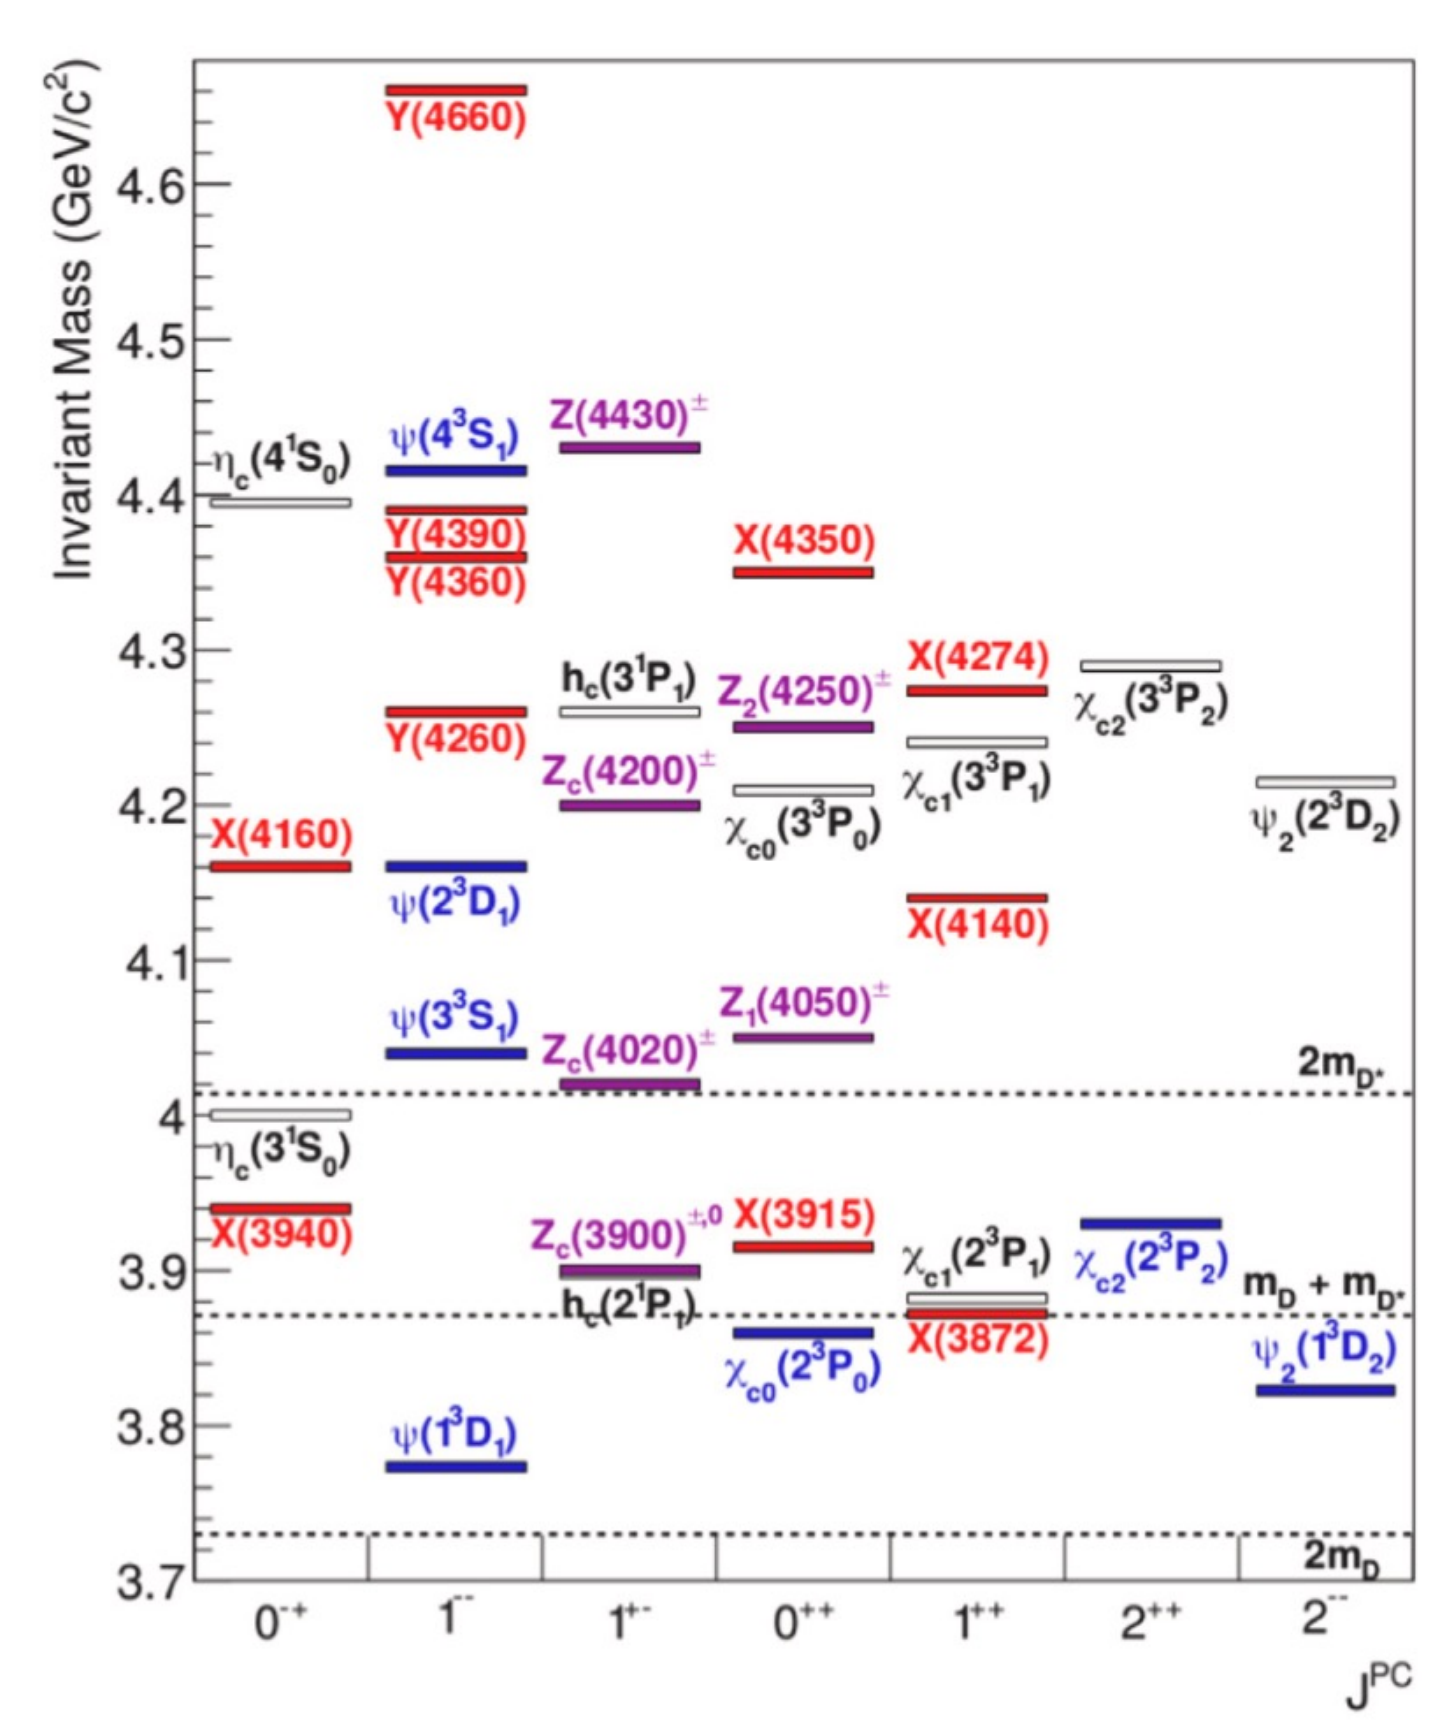
\includegraphics[width=0.95\textwidth]{Figures/xyz_spectrum.pdf}
%   \caption{The $XYZ$ states populating the charmonium region. Established $c\bar c$
%   levels are shown alongside the exotic candidates, many of which cluster near
%   open-charm thresholds.}
%   \label{fig:xyz-spectrum}
% \end{figure}
% ------------------------------------------------------------

\FloatBarrier
\section{}

\subsection{more light meson spesctroscopy}

Glueballs and more eotics in light mesons...

How to see gluons experimentally? Answer: multi-jet events... $g \rightarrow \text{jets}$

2 jets: q qbar (soft gluons)
3 jets: q qbar g (hard gluon)
4 jets: q qbar (g to gg)

lattice: glueball mass spectrum

0++ glueball: problem, remember nonets with two states. Glueball can mix with mesons with same quantum numbers... We must understand mesons to study glueballs

How to hunt for glueballs: 

Supressed in $\gamma$ $\gamma$ collisions... We wont see glueballs in e+e- collisions

Gluon rich processes: central production: Protons pass each other and produce glueball in the middle. Double pomeron exchange

pbar N annihilation at rest:

Stark Mixing... Tune amount of S wave and P wave

multipart final states... 

ppbar at rest to pi+ pi- pi0 

ecample: rho meson...

Dalitz plot... Go to manyy dimentions... 

ppbar to M1 M2 M3 depends on 4x3=12 variables

Energy and momemntum conservation -4
Known masses -3
No preferred directions: -3 euler angles

Total: 2 variables... 2 variables have all the dynamics... Smart choice: invariant masses of both particles...
Result: Dalitz plot...

Angular resolution, that comes from spin of resonance, we can read in the Dalitz plot...

Example: 3 rho bands + f2(1270)

size depends on the available mass you have


\section{Baryon Spectrometry}

Quantum numbers of pi N experiment production (slide 196)

Pi N to R to Pi N

0- 1/2+ (Implies l=0) to S 

S N* J (Mass) 


Old numenclature N(1535)1/2- used to ve S11(1535)
\section{Hadrons structure through electron scattering}
\section{Deep inelastic scattering and the multidimensional structure of the nucleon}
\appendix

\section{Useful tables}\label{app:useful-tables}

This appendix collects the quantities and formulae that recur across the exercise
sheets. Particle masses, widths and branching ratios are \emph{not} reproduced here:
they are maintained by the Particle Data Group and should be looked up at
\url{http://pdglive.lbl.gov}. What follows is the derived material---constituent masses,
naming conventions, kinematic formulae---that is scattered through the chapters and is
tedious to hunt down mid-calculation.

% ------------------------------------------------------------
\subsection{Constituent quark masses}
\label{app:quark-masses}

The constituent masses are effective masses acquired by quarks inside hadrons, and are
much larger than the bare (current) masses generated by the Higgs mechanism. They are the
masses to use in quark-model estimates of magnetic moments and hyperfine splittings.

The current and constituent masses are tabulated in Table~\ref{tab:quark-masses}.
For reference, the values extracted from the baryon magnetic moments in
Sect.~\ref{subsec:magnetic-moments} are $m_u = m_d \approx 327$~MeV and
$m_s \approx 510$~MeV, consistent with the $\sim 350$~MeV and $\sim 500$~MeV
quoted there.

% ------------------------------------------------------------
\subsection{Relativistic kinematics}
\label{app:kinematics}

Collected from Sect.~\ref{subsec:rel-kinematics}. Natural units throughout,
$\hbar = c = 1$. The invariant variables are treated by Halzen and Martin
\cite[Ch.~4]{HalzenMartin1984}, the experimental relations by Perkins
\cite[Ch.~2]{Perkins2000}, and the invariant-mass relations behind the Dalitz entries by
Amsler \cite[App.~B]{Amsler2018}.

\begin{table}[htbp]
    \centering
    \caption{Kinematic relations used throughout the sheets.}
    \label{tab:kinematics}
    \renewcommand{\arraystretch}{1.5}
    \begin{tabular}{ll}
        \hline
        Quantity & Expression \\
        \hline
        Mandelstam invariants
            & $s=(P_1+P_2)^2$, $t=(P_1-P_3)^2$, $u=(P_1-P_4)^2$ \\
        Sum rule
            & $s+t+u=\sum_i m_i^2$ \\
        Virtuality
            & $s$-channel $q^2=s>0$ (timelike); $t$-channel $q^2=t<0$ (spacelike) \\
        Fixed target
            & $s = m_1^2 + m_2^2 + 2 m_2 E_1$ \\
        Real photon on proton
            & $s = M_p^2 + 2 M_p E_\gamma$ \\
        Threshold beam energy
            & $E_1^{\mathrm{thr}} = \dfrac{\left(\sum_f m_f\right)^2 - m_1^2 - m_2^2}{2m_2}$ \\
        Two-body decay energies
            & $E_1 = \dfrac{M^2+m_1^2-m_2^2}{2M}$ \\
        Breakup momentum
            & $|\vec q\,| = \dfrac{\sqrt{[M^2-(m_1+m_2)^2][M^2-(m_1-m_2)^2]}}{2M}$ \\
        Radiative photon energy
            & $E_\gamma = \dfrac{m_i^2-m_f^2}{2m_i}$ \\
        Decay length
            & $d = \beta\gamma\, c\tau = \dfrac{p}{m}c\tau$;\quad
              $N(\ell)=N_0\,e^{-\ell/\beta\gamma c\tau}$ \\
        Track curvature
            & $p\,[\mathrm{GeV}] = 0.3\, B\,[\mathrm{T}]\, R\,[\mathrm{m}]$ \\
        Drell--Yan pair mass
            & $M^2 = x_1 x_2 s$ \\
        \hline
    \end{tabular}
\end{table}

% ------------------------------------------------------------
\subsection{Dalitz plot formulae}
\label{app:dalitz-formulae}

For a parent of mass $M$ decaying to three bodies of masses $m_1$, $m_2$, $m_3$
(Sect.~\ref{subsubsec:dalitz-kinematics}):
\begin{align}
    m_{12}^2 + m_{13}^2 + m_{23}^2 &= M^2 + m_1^2 + m_2^2 + m_3^2, \notag\\
    m_{ij}^2\big|_{\max} &= (M-m_k)^2, \qquad
    m_{ij}^2\big|_{\min} = (m_i+m_j)^2, \notag\\
    m_{23}^2\big|_{\substack{\max\\\min}}
    &= \left(E_2^*+E_3^*\right)^2
       - \left(|\vec p_2^{\,*}| \mp |\vec p_3^{\,*}|\right)^2 .
\end{align}
The sum rule makes the third invariant mass a diagonal axis on a plot of $m_{12}^2$
against $m_{23}^2$. The boundary corresponds to collinear momenta; the interior to
configurations in which the three momenta close into a triangle.

% ------------------------------------------------------------
\subsection{Baryon nomenclature}
\label{app:baryon-naming}

Baryons are named by isospin and strangeness (Sect.~\ref{subsec:baryon-naming}):
$N$ ($I=\tfrac12$, $S=0$), $\Delta$ ($I=\tfrac32$, $S=0$), $\Lambda$ ($I=0$, $S=-1$),
$\Sigma$ ($I=1$, $S=-1$), $\Xi$ ($I=\tfrac12$, $S=-2$), $\Omega$ ($I=0$, $S=-3$).

The older $\pi N$ scattering notation $L_{2I\,2J}(\text{mass})$ uses spectroscopic
letters for $L$ and \emph{twice} the isospin and total angular momentum as subscripts;
the conversion to modern names is tabulated in Table~\ref{tab:l2i2j}. Parity follows from
$P=(-1)^{L+1}$, so $S$ and $D$ waves are negative-parity and $P$ and $F$ waves positive.

Clebsch--Gordan coefficients for the couplings needed on the sheets
($\tfrac12\otimes\tfrac12$, $1\otimes\tfrac12$, $\tfrac32\otimes\tfrac12$,
$1\otimes 1$, $\tfrac32\otimes 1$, $2\otimes\tfrac12$) are reproduced in
Fig.~\ref{fig:cg_table}.

% ------------------------------------------------------------
\subsection{Exercise sheet cross-reference}
\label{app:sheet-map}

Where to look for the material behind each exercise. Sheet numbers refer to the
SS~2026 problem sets.

\begin{longtable}{llL{7.2cm}}
    \hline
    Sheet & Topic & Sections \\
    \hline
    \endhead
    1.1 & Standard Model particles      & Sect.~\ref{subsec:history-quark-model} \\
    1.2 & Spin addition                 & Sect.~\ref{subsec:addition} \\
    1.3 & Yukawa range                  & Sect.~\ref{subsec:yukawa} \\
    1.4 & Feynman diagrams, $s$/$t$ channel & Sect.~\ref{subsubsec:mandelstam} \\
    \hline
    2.1 & Cross section, luminosity     & Sect.~\ref{subsec:scattering-reminder} \\
    2.2 & Invariant mass from $2\gamma$ & Sect.~\ref{subsec:invariant-mass} \\
    2.3 & Bubble chamber, curvature     & Sect.~\ref{subsec:bubble-chamber} \\
    2.4 & Parity of the charged pion    & Sect.~\ref{subsec:pion-parity} \\
    2.5 & Missing mass                  & Sect.~\ref{subsec:invariant-mass} \\
    \hline
    3.1 & Isospin, $\pi N$ system       & Sect.~\ref{subsec:su2},
                                          Eq.~\eqref{eq:piN-decomposition} \\
    3.2 & Strangeness production, thresholds & Sect.~\ref{subsubsec:thresholds},
                                          Sect.~\ref{subsec:accelerator-discovery} \\
    3.3 & Young tableaux                & Sect.~\ref{subsec:youngtableaux} \\
    \hline
    4.1 & Gell-Mann--Okubo              & Sect.~\ref{subsec:gmo},
                                          Sect.~\ref{subsec:gmo-mesons} \\
    4.2 & Bubble chamber                & Sect.~\ref{subsec:bubble-chamber} \\
    4.3 & $C$, $G$, $P$ at work         & Sect.~\ref{subsec:qnumbers},
                                          Sect.~\ref{subsubsec:bose-symmetry} \\
    4.4 & Ideal mixing                  & Sect.~\ref{subsec:nonets} \\
    \hline
    5.1 & Meson wavefunctions           & Sect.~\ref{subsec:qnumbers} \\
    5.2 & Baryon wavefunctions          & Sect.~\ref{subsec:baryon-antisymmetry},
                                          Sect.~\ref{subsec:su6-56plet} \\
    5.3 & $N$ and $\Delta$ spectrum     & Sect.~\ref{subsec:supermultiplets},
                                          Table~\ref{tab:70-1minus} \\
    5.4 & $J/\psi$ width and $\alpha_s$ & Sect.~\ref{subsec:ozi-width},
                                          Sect.~\ref{subsec:resonances} \\
    \hline
    6.1 & Breit--Wigner, Argand         & Sect.~\ref{subsec:resonances} \\
    6.2 & Quarkonium widths, $\alpha_s$ & Sect.~\ref{subsec:qq-potential},
                                          Sect.~\ref{subsec:ozi-width} \\
    6.3 & The missing $c\bar c$ state   & Sect.~\ref{subsec:charmonium-probes} \\
    6.4 & Properties of the $J/\psi$    & Sect.~\ref{subsec:jpsi-discovery},
                                          Sect.~\ref{subsec:ozi} \\
    \hline
    7.1 & Constituent quark masses      & Sect.~\ref{subsec:magnetic-moments} \\
    7.2 & $\bar p N$ annihilation       & Sect.~\ref{subsec:annihilation},
                                          Sect.~\ref{subsubsec:bose-symmetry} \\
    7.3 & Dalitz plot from data         & Sect.~\ref{subsec:dalitz} \\
    \hline
    8.1 & Dalitz plot                   & Sect.~\ref{subsubsec:dalitz-kinematics} \\
    8.2 & Three-body decays             & Sect.~\ref{subsubsec:dalitz-kinematics} \\
    8.3 & Exotic mesons                 & Sect.~\ref{subsec:gluonic_matter} \\
    \hline
    9.1 & CMS momenta at the boundary   & Sect.~\ref{subsubsec:twobody},
                                          Sect.~\ref{subsubsec:dalitz-kinematics} \\
    9.2 & Baryon naming scheme          & Sect.~\ref{subsec:baryon-naming} \\
    9.3 & Isospin in weak decays        & Sect.~\ref{subsec:deltaI-half} \\
    \hline
    10.1 & Spectroscopic notation       & Table~\ref{tab:l2i2j} \\
    10.2 & Vector meson dominance       & Sect.~\ref{subsec:vmd} \\
    10.3 & Double polarization          & Sect.~\ref{subsec:double-polarization} \\
    10.4 & $\gamma\gamma$ decays        & Sect.~\ref{subsec:qnumbers} \\
    \hline
    11.1 & Dalitz plots, $\sqrt{s}$     & Sect.~\ref{subsubsec:thresholds} \\
    11.2 & Form factors                 & Sect.~\ref{subsec:form-factors} \\
    11.3 & Properties of the nucleon    & Sect.~\ref{subsec:rosenbluth},
                                          Sect.~\ref{subsec:neutron-ff} \\
    \hline
    12.1 & Deep inelastic scattering    & Sect.~\ref{subsec:inclusive-kinematics},
                                          Sect.~\ref{subsec:parton-model} \\
    12.2 & Discovery of $W$ and $Z$     & Sect.~\ref{subsubsec:wz-discovery} \\
    12.3 & Callan--Gross relation       & Eq.~\eqref{eq:callan-gross} \\
    12.4 & Neutrino nucleon DIS         & Eq.~\eqref{eq:nu-beam-production} ff. \\
    \hline
    13.1 & Scaling violation            & Sect.~\ref{subsec:dglap} \\
    13.2 & The $\eta$ meson, thresholds & Sect.~\ref{subsec:eta-gateway},
                                          Sect.~\ref{subsubsec:thresholds} \\
    13.3 & Pentaquarks                  & Sect.~\ref{subsec:insight-outlook} \\
    13.4 & Baryon wavefunction symmetry & Sect.~\ref{subsec:baryon-antisymmetry},
                                          Sect.~\ref{subsec:supermultiplets} \\
    \hline
\end{longtable}


% Bibliography (BibTeX)
\bibliographystyle{unsrt}
\bibliography{references}


\end{document}


